%%% FILE WITH ALL TABLES DEFINITIONS %%%

%%% EXAMPLE TABLE %%%
\renewcommand{\Tabladeejemplo}{
    \begin{table}[h]
        \centering
        \caption{Caption for the table.}
        \label{tab:example_table}
        \begin{tabularx}{\textwidth}{XXX} % Removed the extra brackets
            \toprule
            Column 1 & Column 2 & Column 3 \\ \midrule
            Data 1 & Data 2 & Data 3 \\
            Data 4 & Data 5 & Data 6 \\
            \bottomrule
        \end{tabularx}
    \end{table}
}

%%% APPROVAL TABLE %%%
\renewcommand{\approvaltable}{
    \begin{center}
        \begin{table}[ht]
            \begin{tabularx}{\textwidth}{lXXX}
            \toprule
            \textbf{Title}        & \multicolumn{3}{l}{\textbf{FYS DRD and Guidelines}}   \\ \midrule
            Issue Number & 1                      & Revision Number  & 0 \\ 
            Author       &  Edgar Hernandez Recio                      & Date             &   \\ 
            Approved By  &                        & Date of Approval &   \\ 
            \bottomrule
            \end{tabularx}
            \label{tab:approval}
        \end{table}
    \end{center}
}

%%% APPROVAL TABLE %%%
\renewcommand{\changelogtable}{
    \begin{center}
        \begin{table}[ht]
            \begin{tabularx}{\textwidth}{lXXX}
            \toprule
            Reason for change   & Issue Nr  & Revision Number   & Date  \\ \midrule
            First release       & 1         & 0                 &       \\ 
            Second release      & 2         & 0                 &       \\
            \bottomrule
            \end{tabularx}
            \label{tab:change_log}
        \end{table}
    \end{center}
}

%%% APPROVAL TABLE %%%
\renewcommand{\recordtable}{ 
    \begin{center}
        \begin{table}[ht]
            \begin{tabularx}{\textwidth}{lXXX}
            \toprule
            \textbf{Issue Number}   & \multicolumn{3}{l}{\textbf{Revision Number}}  \\ \midrule
            Issue Number            & 1         & Revision Number   & 0             \\ \midrule
            Reason for change       & Date      & Pages             & Paragraph(s)  \\ \midrule
            First release           &           &                   &               \\
            Second release          &           &                   &               \\
            \bottomrule
            \end{tabularx}
            \label{tab:change_record}
        \end{table}
    \end{center}
}

%%% DISTRIBUTION TABLE %%%
\renewcommand{\distributiontable}{
    \begin{center}
        \begin{table}[ht]
            \begin{tabularx}{\textwidth}{X}
            \toprule
            \textbf{Disclaimer} \\ \midrule
            This document has been prepared for use by the Fly Your Satellite! PoCat Lektron team.\\
            \textbf{This document shall be considered confidential and not to be distributed further without permission of ESA Education, and the authors.}   \\ \bottomrule
            \end{tabularx}
            \label{tab:distribution}
        \end{table}
    \end{center}
}

%%% Table for the sensors and actuators %%%
\renewcommand{\sensorsactuators}{
    \begin{table}[h]
        \centering
        \begin{tabular}{ll}
            \hline
            \textbf{Sensors}      & \textbf{Actuator}     \\ \hline
            Gyroscope    & Magnetorquer \\
            Photodiodes  &              \\
            Magnetometer &              \\ \hline
        \end{tabular}
    \end{table}
}
%%% Table for the magnetorquer description %%%
\renewcommand{\magnetorquercharacteristics}{
    \begin{table}[htbp]
    \centering
        \begin{tabularx}{0.9\linewidth}{X c c c c}
            \toprule
            \textbf{Board} & \textbf{Turns} & \textbf{Max moment (A$\cdot$m$^2$)} & \textbf{Dimensions (mm$\times$mm)} & \textbf{Layers} \\
            \midrule
            Top & 42$\times$layer & $9.17 \times 10^{-4}$ & 32 $\times$ 32 & 4 \\
            Bottom \& Lateral & 38$\times$layer & 0.0017 & 32 $\times$ 32 & 4 \\
            \bottomrule
        \end{tabularx}
    \end{table}
}
\section{Simulation model}
To assist the Attitude and Orbit Control System (AOCS) design, verification and validation, a simulation model using mathlab code has been used. The
simulation is based on the Princeton Toolbox (PT) \cite{PrincetonToolbox}, which contains a set of functions and 
simulations initially created for CubeSats, that has been adapted to the PocketQube (PQ).

\subsection{PocketQube Model}
The mission is formed by two PQs, one using an L-band Radiometer and the other using a K-band radiometer. To model the PQ, a 3 dimensional cube has
been used, shown in \textit{Figure \ref{fig:PQmodel}}. This cube has the same dimensions as a PQ 5x5x5 cm$^2$ and the same mass as the PQs. Additionally, to apply the inertia of the PQs, the 
inertia matrix is taken into account in the simulation.\vspace{0.2em}

\noindent The satellites will be simulated in two different configurations, on the one hand in stowed configuration (without the anntennas deployed) and on the other
hand in deployed configuration. In the case of the L-band PQ the stowed configuration contains both the L-band antenna and communications antenna
stowed.
    \begin{figure}[H]
        \centering
        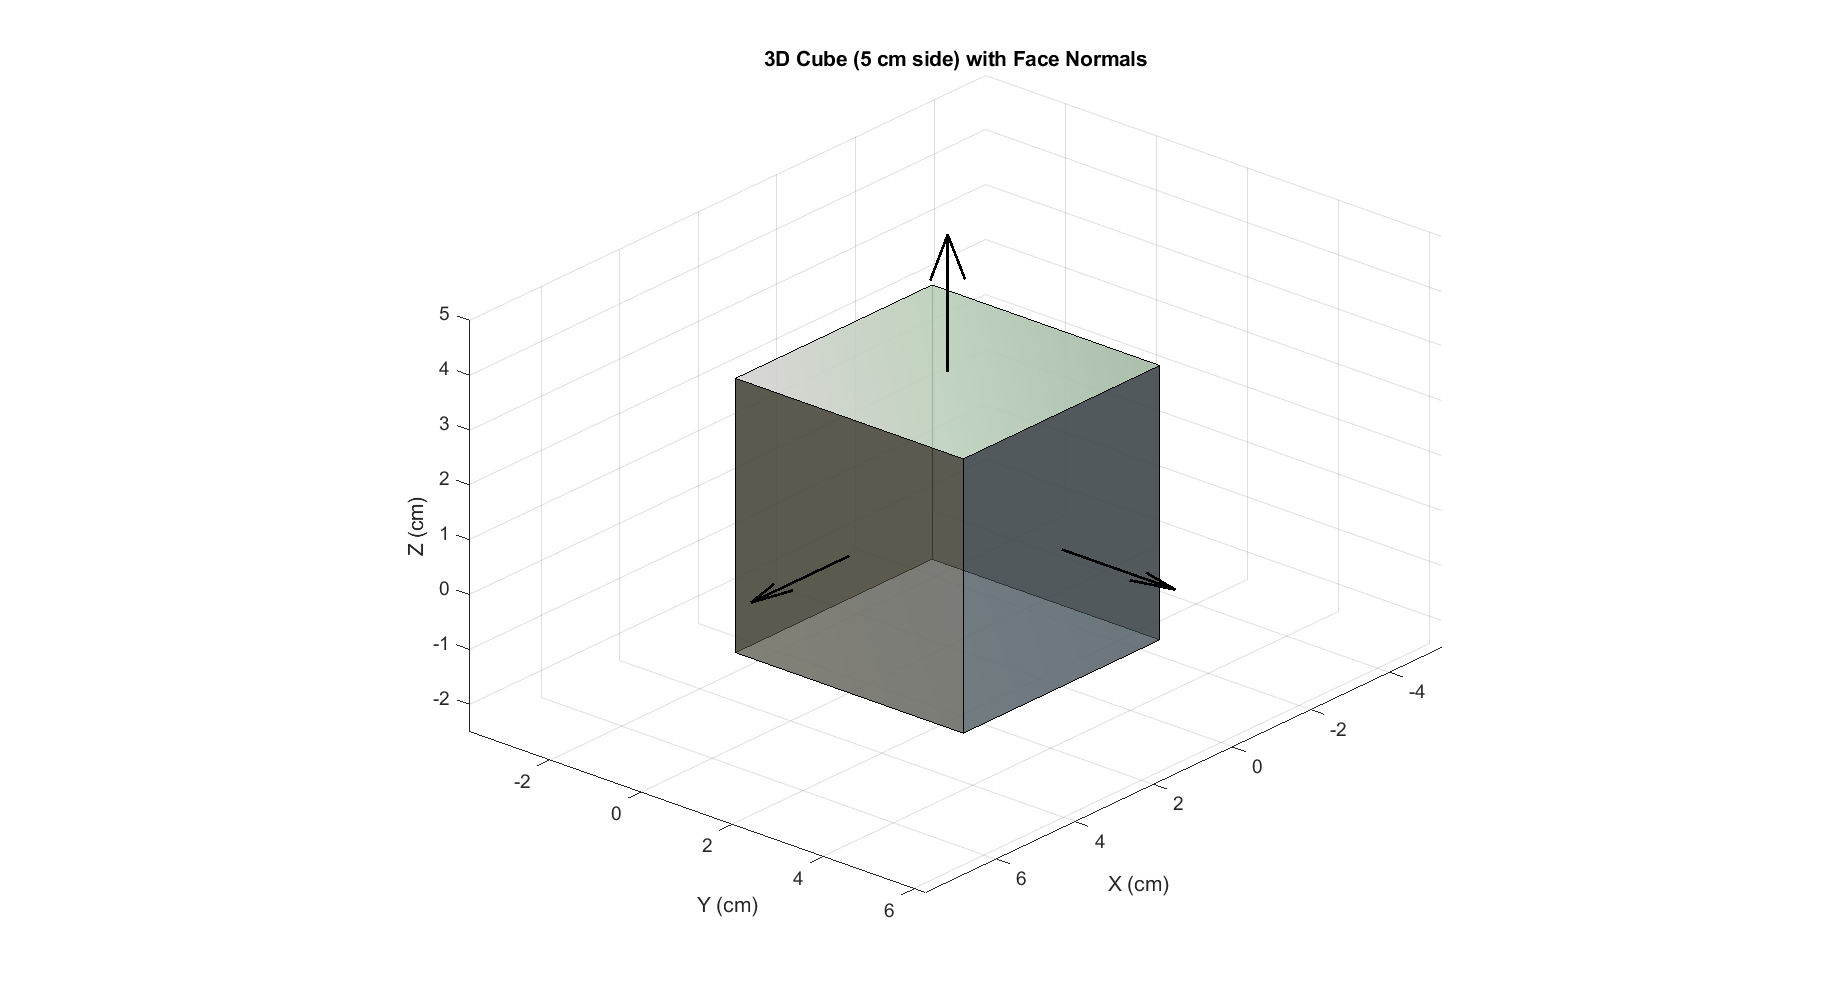
\includegraphics[width=0.8\linewidth]{res/img/3_simulation_performance/PQ model.png}
        \caption{PQ 3D model}
        \label{fig:PQmodel}
    \end{figure}

\subsection{Environmental model and asumptions}

\subsubsection{Reference frames}
\begin{itemize}
    \item \textbf{Earth Centered Inertial (ECI) frame:}\\
    The ECI frame is a global cartesian reference frame that has its origin at the centre of the
    Earth.
    \begin{itemize}
        \item X axis points to the Vernal Equinox.
        \item Y axis completes the set with the right-hand rule.
        \item Z axis aligned with the Earth's rotation axis.
    \end{itemize}

    \begin{figure}[H]
        \centering
        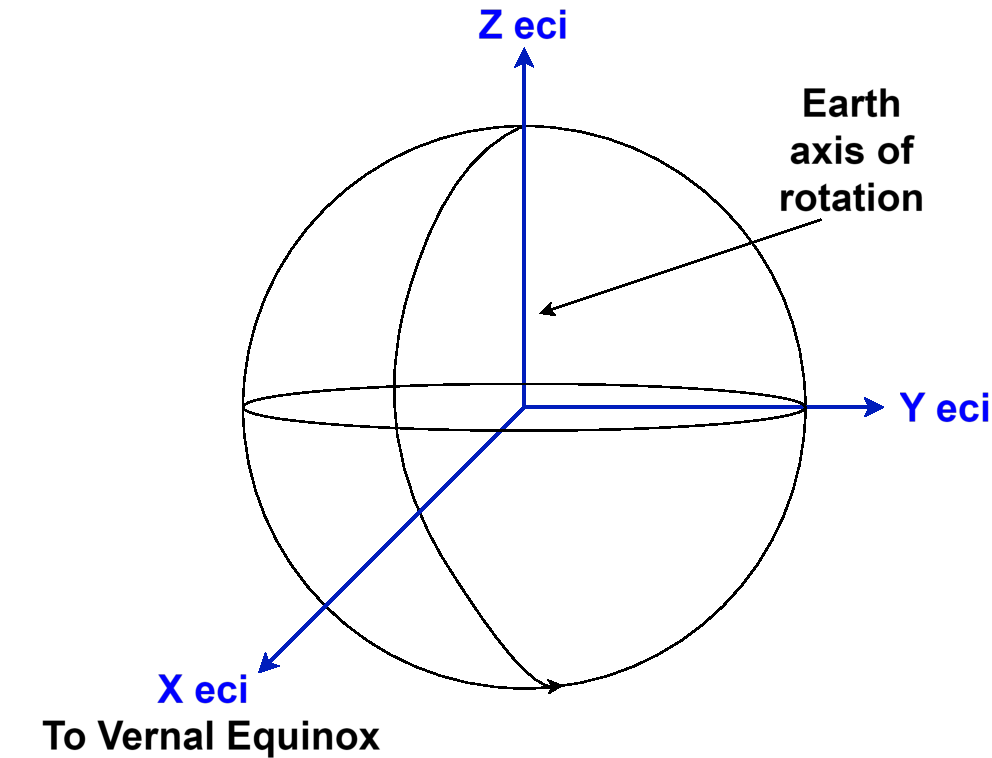
\includegraphics[width=0.4\linewidth]{res/img/3_simulation_performance/ECI frame.drawio.pdf}
        \caption{ECI frame representation}
        \label{fig:ECIframe}
    \end{figure}

    \item \textbf{Body frame:}\\
    The Body frame is a global cartesian reference frame that has its origin at the centre of
    the PQ.
    \begin{itemize}
        \item X axis aligned with the PQ width, parallel to the sliding plate and perpendicular
        to the direction of insertion into the PQ deployer.
        \item Y axis aligned with the PQ length, the direction of insertion into the
        PQ deployer and completing the right handed reference frame.
        \item Z axis aligned with the PQ height direction, pointing upwards from the
        sliding plate.

    \end{itemize}

    \begin{figure}[H]
        \centering
        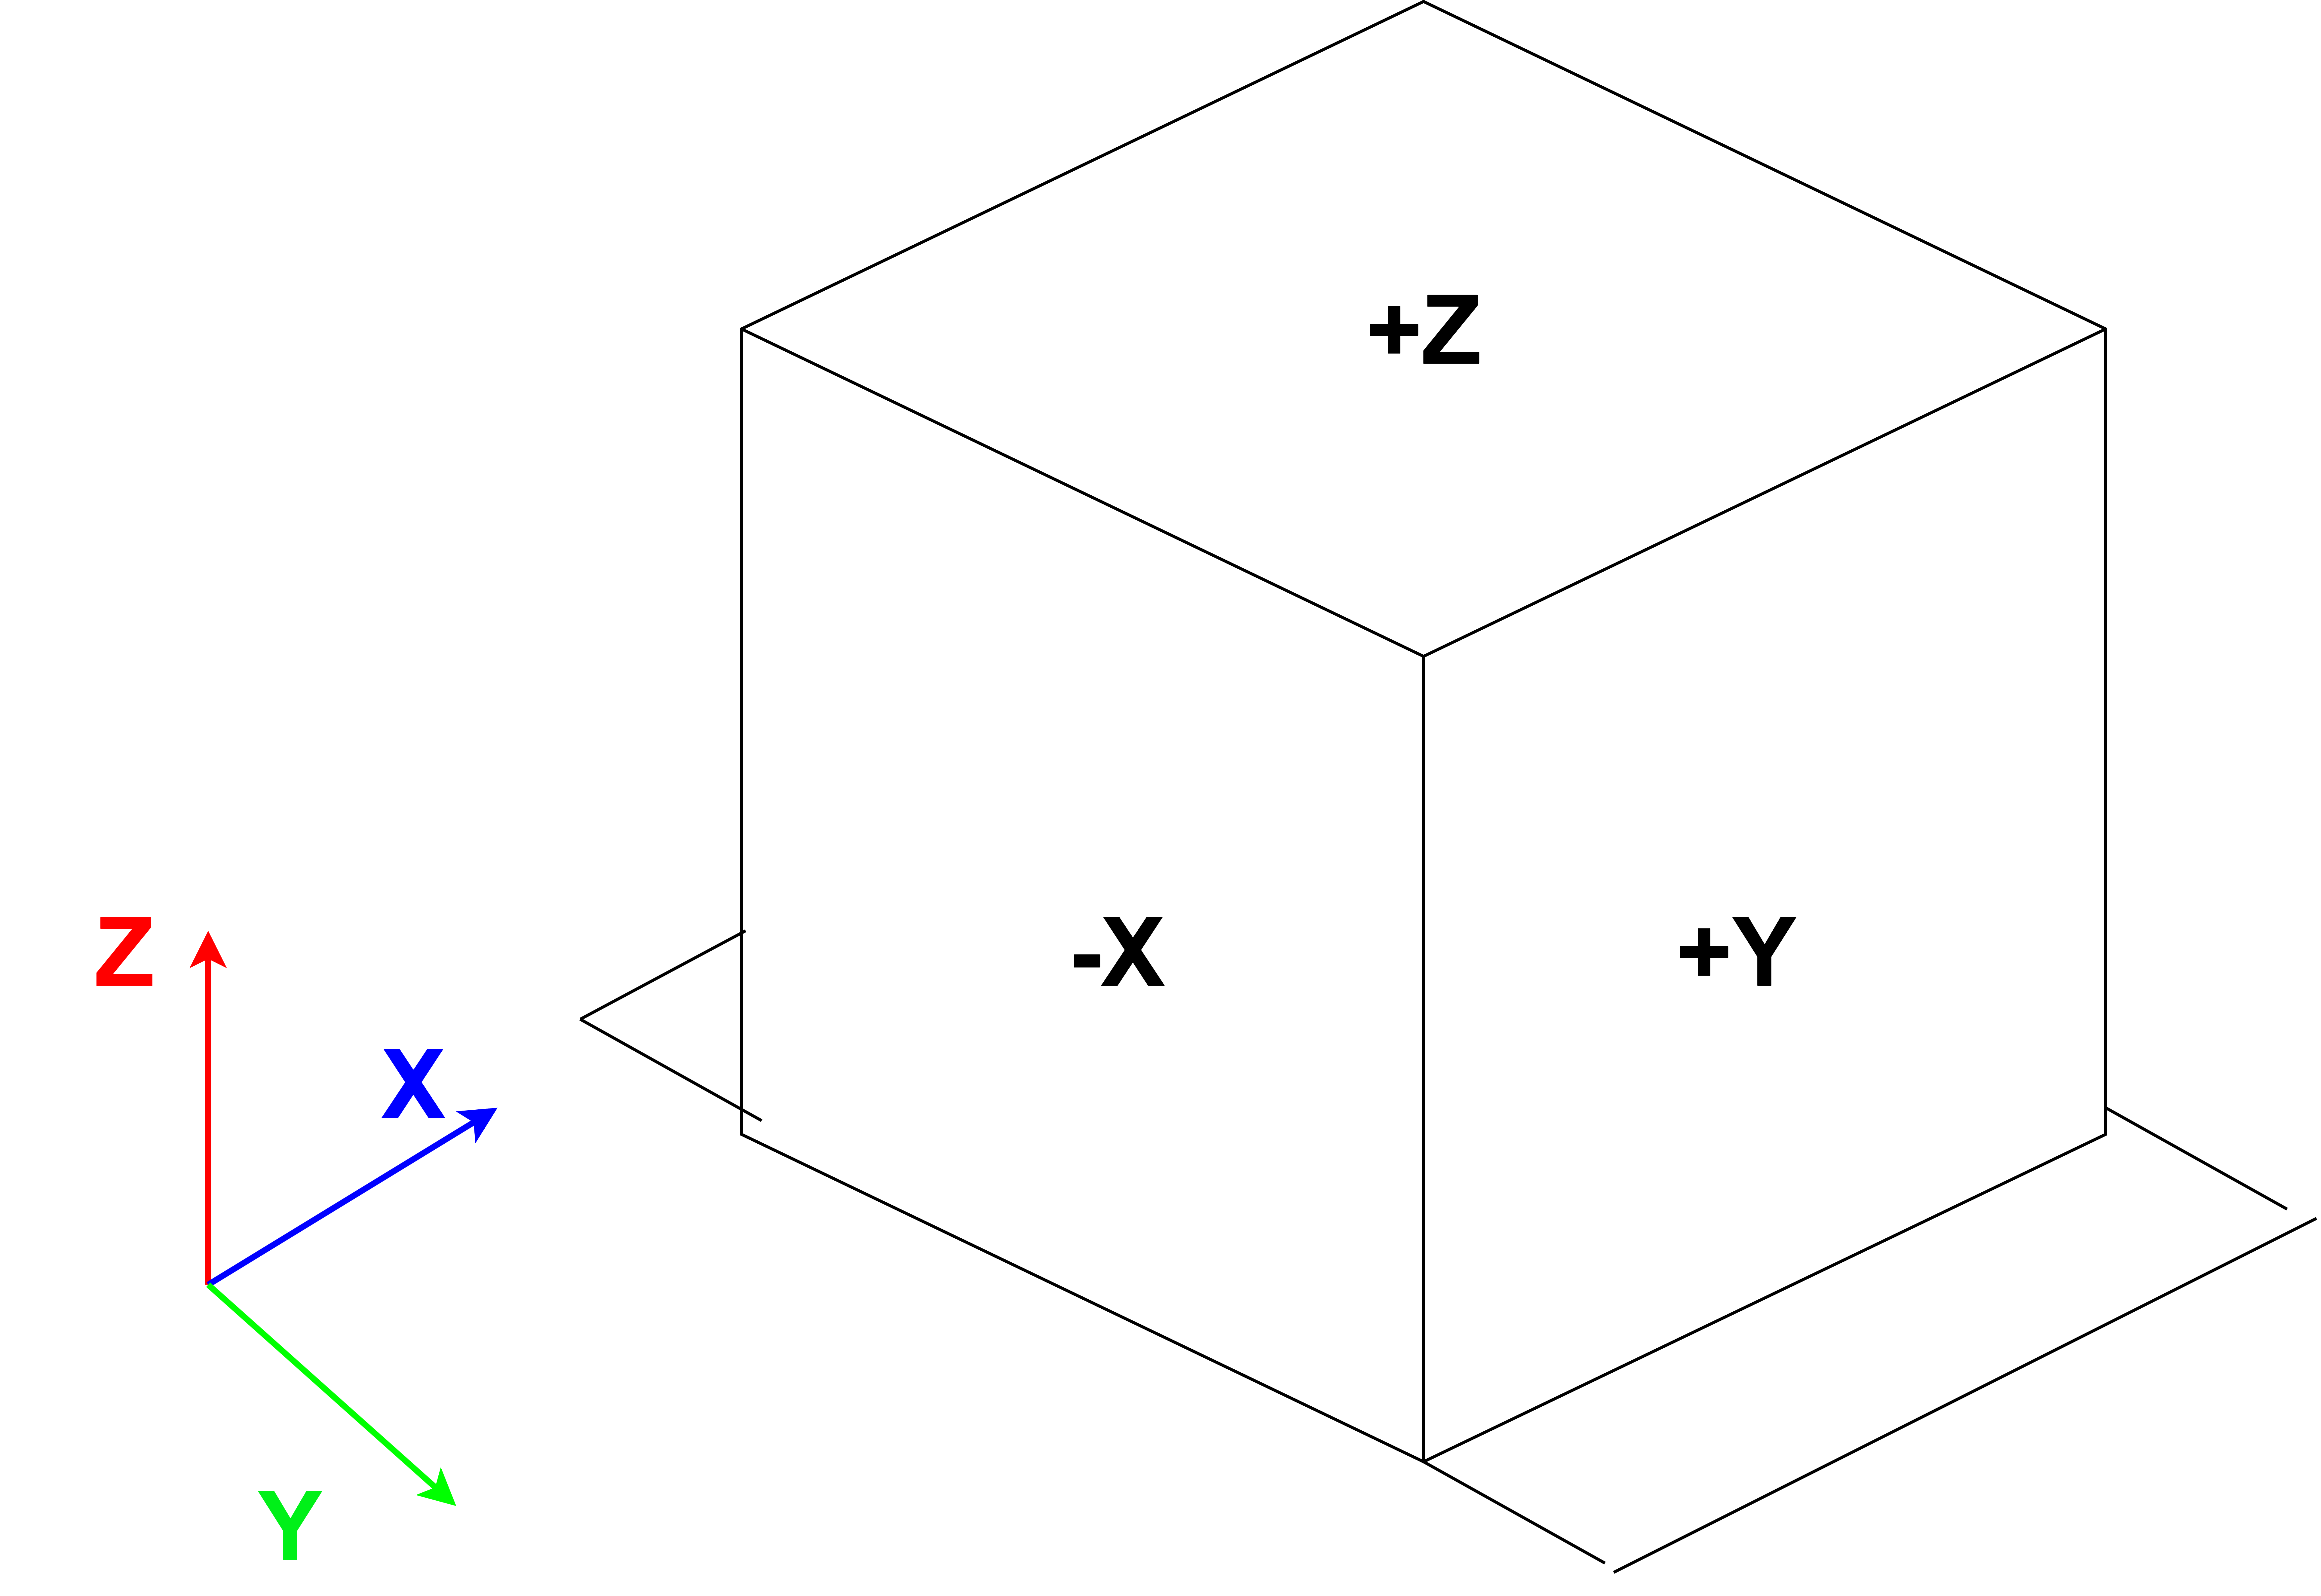
\includegraphics[width=0.4\linewidth]{res/img/3_simulation_performance/bodyframe.drawio.png}
        \caption{Body frame representation}
        \label{fig:ECIframe}
    \end{figure}

    \item \textbf{Local Vertical Local Horizontal (LVLH) Frame:}\\
    The LVLH Frame will be mainly used for results presentation in the Nadir pointing simulations. The frame is described as:
    \begin{itemize}
        \item X-Axis: Perpendicular to Y and Z, forming a right-handed coordinate system - Local Horizontal
        \item Y-Axis: Negative to the orbit normal, or in the direction of -h
        \item Z-Axis: Oriented in the direction of -r (points to center of Earth) - Local Vertical
    \end{itemize}

    \begin{figure}[H]
        \centering
        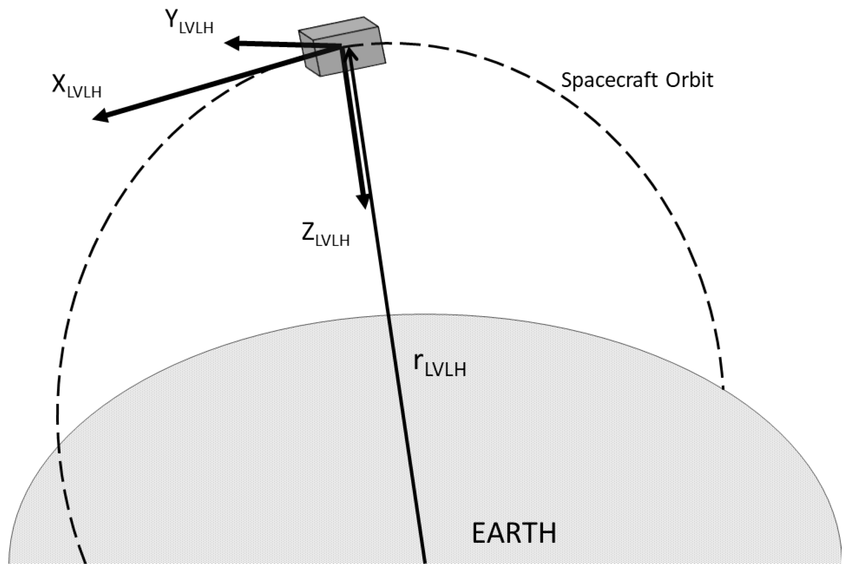
\includegraphics[width=0.4\linewidth]{res/img/3_simulation_performance/LVLH-Local-Vertical-Local-Horizontal-frame-definition.png}
        \caption{LVLH frame representation}
        \label{fig:ECIframe}
    \end{figure}
\end{itemize}

\subsubsection{Environmental models}
The following environmental models are used in the simulation:
\begin{itemize}
    \item \textbf{Earth's magnetic field model \cite{Tilted_Dipole}:} The Earth's magnetic field model used in the simulation is based
    on the Tilted dipole mode, which includes the effect of the dipole motion of the Earth.
    \item \textbf{Aerodynamic Drag model:} The simulation uses an aerodinamic drag model based on the Jacchia's 1970 model
    \cite{J70_atmosphere}. 
    \item \textbf{Radiation Pressure model:} The simulation includes the solar radiation pressure, the earth radiation
    pressure and the earth albedo pressure.
    \item \textbf{Gravity field model:} The simulation accounts for a point-mass gravity model.
\end{itemize}

\subsubsection{External disturbances}
The following external disturbances are considered in the simulation:
\begin{itemize}
    \item \textbf{Drag force:} 
    \item \textbf{Aerodynamic torques:} 
    \item \textbf{Gravity gradient torques:} 
    \item \textbf{Radiation Torques:} 
\end{itemize}

\subsection{Orbit and attitude kinematic propagators}

As for the Orbit propagator in the simulation, firstly, the used equations or motion are the Cowell'
form of the two body problem, using  disturbances. In addition, the integrator type used is the Runge-Kutta 4th order method.
As for the propagation of the parameters, they are done in the ECI frame.\vspace{0.2em}

\noindent The parameters included in the initial vector for describing the state of the satellite at the begining of the simulation are:

\begin{itemize}
    \item Satellite's position.
    \item Satellite's velocity.
    \item Satellite's attitude quaternion.
    \item Satellite's angular velocity.
\end{itemize}

\noindent Regarding the attitude representation of the satellite in the simulation, the mathematical expresion that will be used is the quaternion. During the
simulation the quaternion that will be used is the one representing the rotation fromt he body frame to the ECI frame. However, at the time to 
present the results the quaternion that will be used will be the one representing a rotation from the LVLH frame to the ECI frame.

\subsection{Sensor and actuator models}
In this section all the models used for the sensors and for the actuators are described. It is assumed that all the sensors has been calibrated
and temperature characterized. A brief list of the sensors and actuators included in the PQ is presented below:

\sensorsactuators

\subsubsection{Gyroscope}
The model used to represent the gyroscope output given by \cite{Landis} is:

\begin{equation}
    \boldsymbol{\omega} = \boldsymbol{\omega_o} +\boldsymbol{b(t)}+\boldsymbol{n},
\end{equation}
where:
\begin{itemize}
    \item $\boldsymbol{\omega}$ is the measured angular velocity vector.
    \item $\boldsymbol{\omega_o}$ is the true angular velocity of the satellite.
    \item $\boldsymbol{b}$ is the bias term, modeled as a random walk process.
    \item $\boldsymbol{n}$ is a zero-mean Gaussian noise vector.
\end{itemize}
\subsubsection{Photodiodes}

The output of the photodiodes can be modeled as:

\begin{equation}
    \boldsymbol{v} = \boldsymbol{v_o(T)} + \boldsymbol{n}
\end{equation}

where:
\begin{itemize}
    \item $\boldsymbol{v}$ is the measured voltage output vector,
    \item $\boldsymbol{v_o(T)}$ is the true signal component that is dependent to the temperature $\boldsymbol{T}$ previously calibrated.
    \item $\boldsymbol{n}$ represents additive noise, typically modeled as zero-mean Gaussian noise.
\end{itemize}

\subsubsection{Magnetometer}

The magnetometer model is expressed as:

\begin{equation}
\boldsymbol{B}_{\text{meas}} = \left( \mathbf{C}_e \cdot \boldsymbol{B}_{\text{true}} \right) + \boldsymbol{b}_e + \boldsymbol{n}
\end{equation}

where:

\begin{itemize}
    \item $\boldsymbol{B}_{\text{meas}}$ is the measured magnetic field vector in the body frame.
    \item $\boldsymbol{B}_{\text{true}}$ is the true magnetic field vector in the body frame.
    \item $\mathbf{C}_e$ is the calibration matrix with errors.
    \item $\boldsymbol{b}_e$ is the sensor bias error vector.
    \item $\boldsymbol{n}$ is zero-mean Gaussian white noise with known variance.
\end{itemize}

\subsubsection{Magnetorquer}
The magnetorquers are simulated as a mathematical formula. The magnetorquers generate a magnetic moment depending on the injected intensity, therefore,
in the simulation this magnetic moment is calculated and later used to propagate the following attitude of the satellite with the other external disturbances.
The formula used for calculating the magnetic moment generated by the magnetorquers is:

\begin{equation}
    \boldsymbol{m}=I_o·N_{layers}·\sum_{i=1}^{N_{turns}}(l-2(i-1)(w+d))^2
\end{equation}

\noindent Where the $l$ is the length of the magnetorquer, the $w$ the width of the copper trail, the $d$ the distance between trails, $N_{layers}$ is the number
layers in which the magnetorquer is divided and $N_{turns}$ is the number of turns in the magnetorquer. The $I_o$ is the injected current, which is the input of the magnetorquer. 
The table below shows the characteristics of the magnetorquers used in the simulation:

\magnetorquercharacteristics



\subsection{Simulaton / model sampling times and frequencies}
The simulation time used is 2 seconds which corresponds to 0.5 Hz. This is due to the fact that the On Board Computer (OBC) used in the PQ
only has one thread to manage all the tasks, therefore, the sampling frequency has been chosen thinking in the worst case scenario. The 
sampling time of the sensors is the same one as the simulation time.

\section{Simulation performance campaign plan and results}

In this section the simulation results of the two different operational modes of the ADCS in the PQ are presented.

\subsection{Nadir Pointing Mode}

The objective of the Nadir Pointing is to point the Payload located at the top board of the PQ towards the Earth, so that 
the Payload can take measurements of the Earth. For this mode the following requirements have been defined: \vspace{1em}


\noindent \textit{The Absolute Performance Error (APE) of the Payload boresight shall be less than 20º with respect to the Y and X 
axes, which are the axes perpendicular to the boresight, and this requirement should be met for 95\% of the time.} \vspace{1em}


\subsubsection{Assumptions and limitations}
The list below presents the different assumptions and aspects considered to perform the simulations.
\begin{itemize}
    \item \textbf{Orbit parameters}
    \begin{itemize}
        \item Inclination: 90 degrees
        \item Altitude: 500 Km
        \item Eccentricity: 0 degrees
        \item Initial satellite position: [ 6887 , 0 , 0 ] Km
        \item Initial satellite velocity: [ 0 , 0 , 7.6 ] Km/s
        \begin{figure}[H]
            \centering
            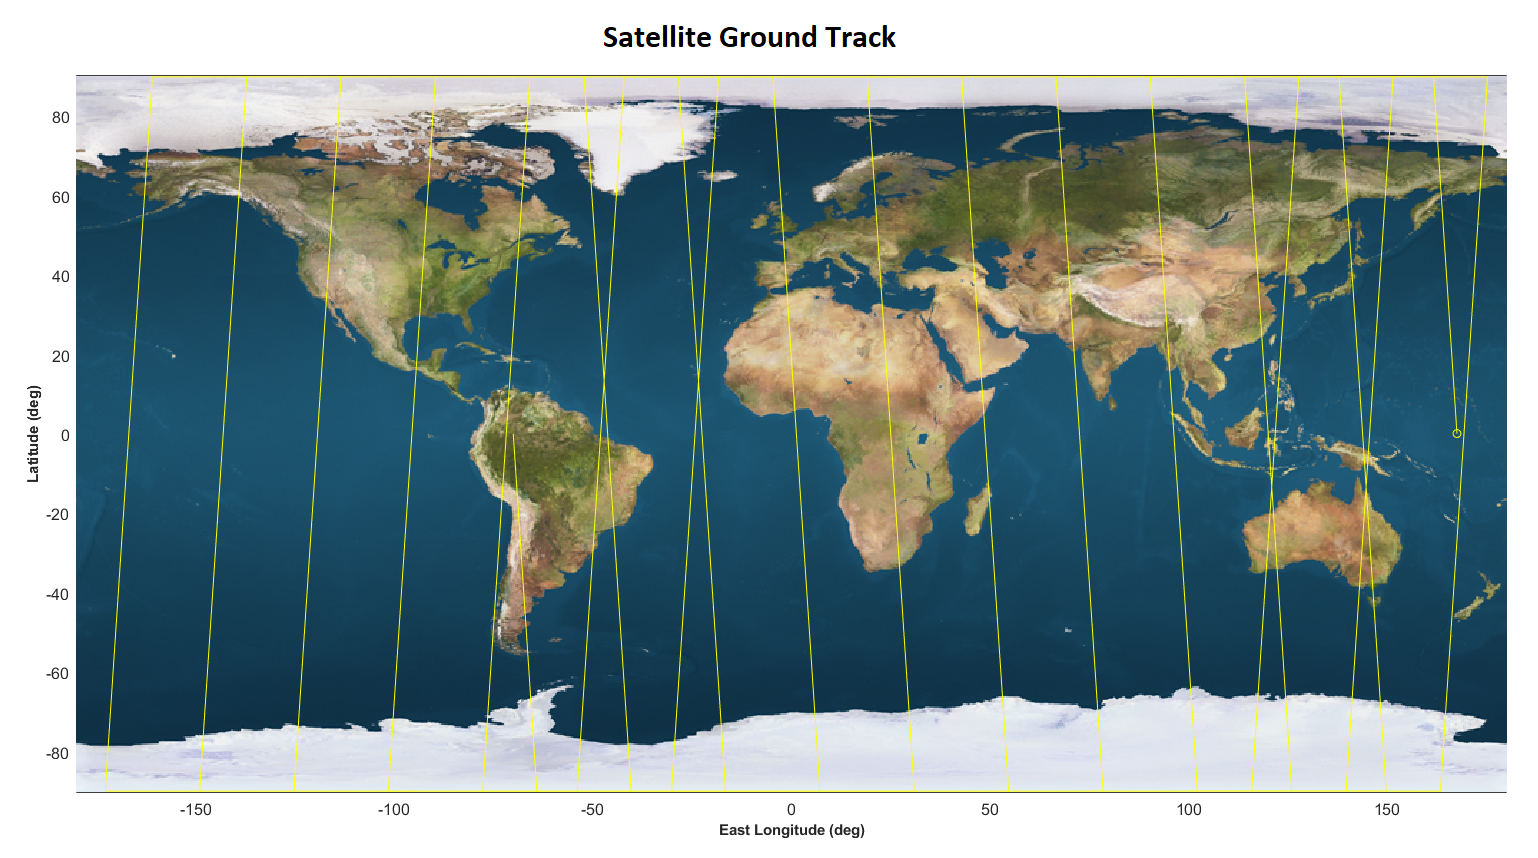
\includegraphics[width=0.8\linewidth]{res/img/3_simulation_performance/Sat_groundtrack.png}
            \caption{Ground track of the simulated PQ orbit}
            \label{fig:GTrack}
        \end{figure}

        \begin{figure}[H]
            \centering
            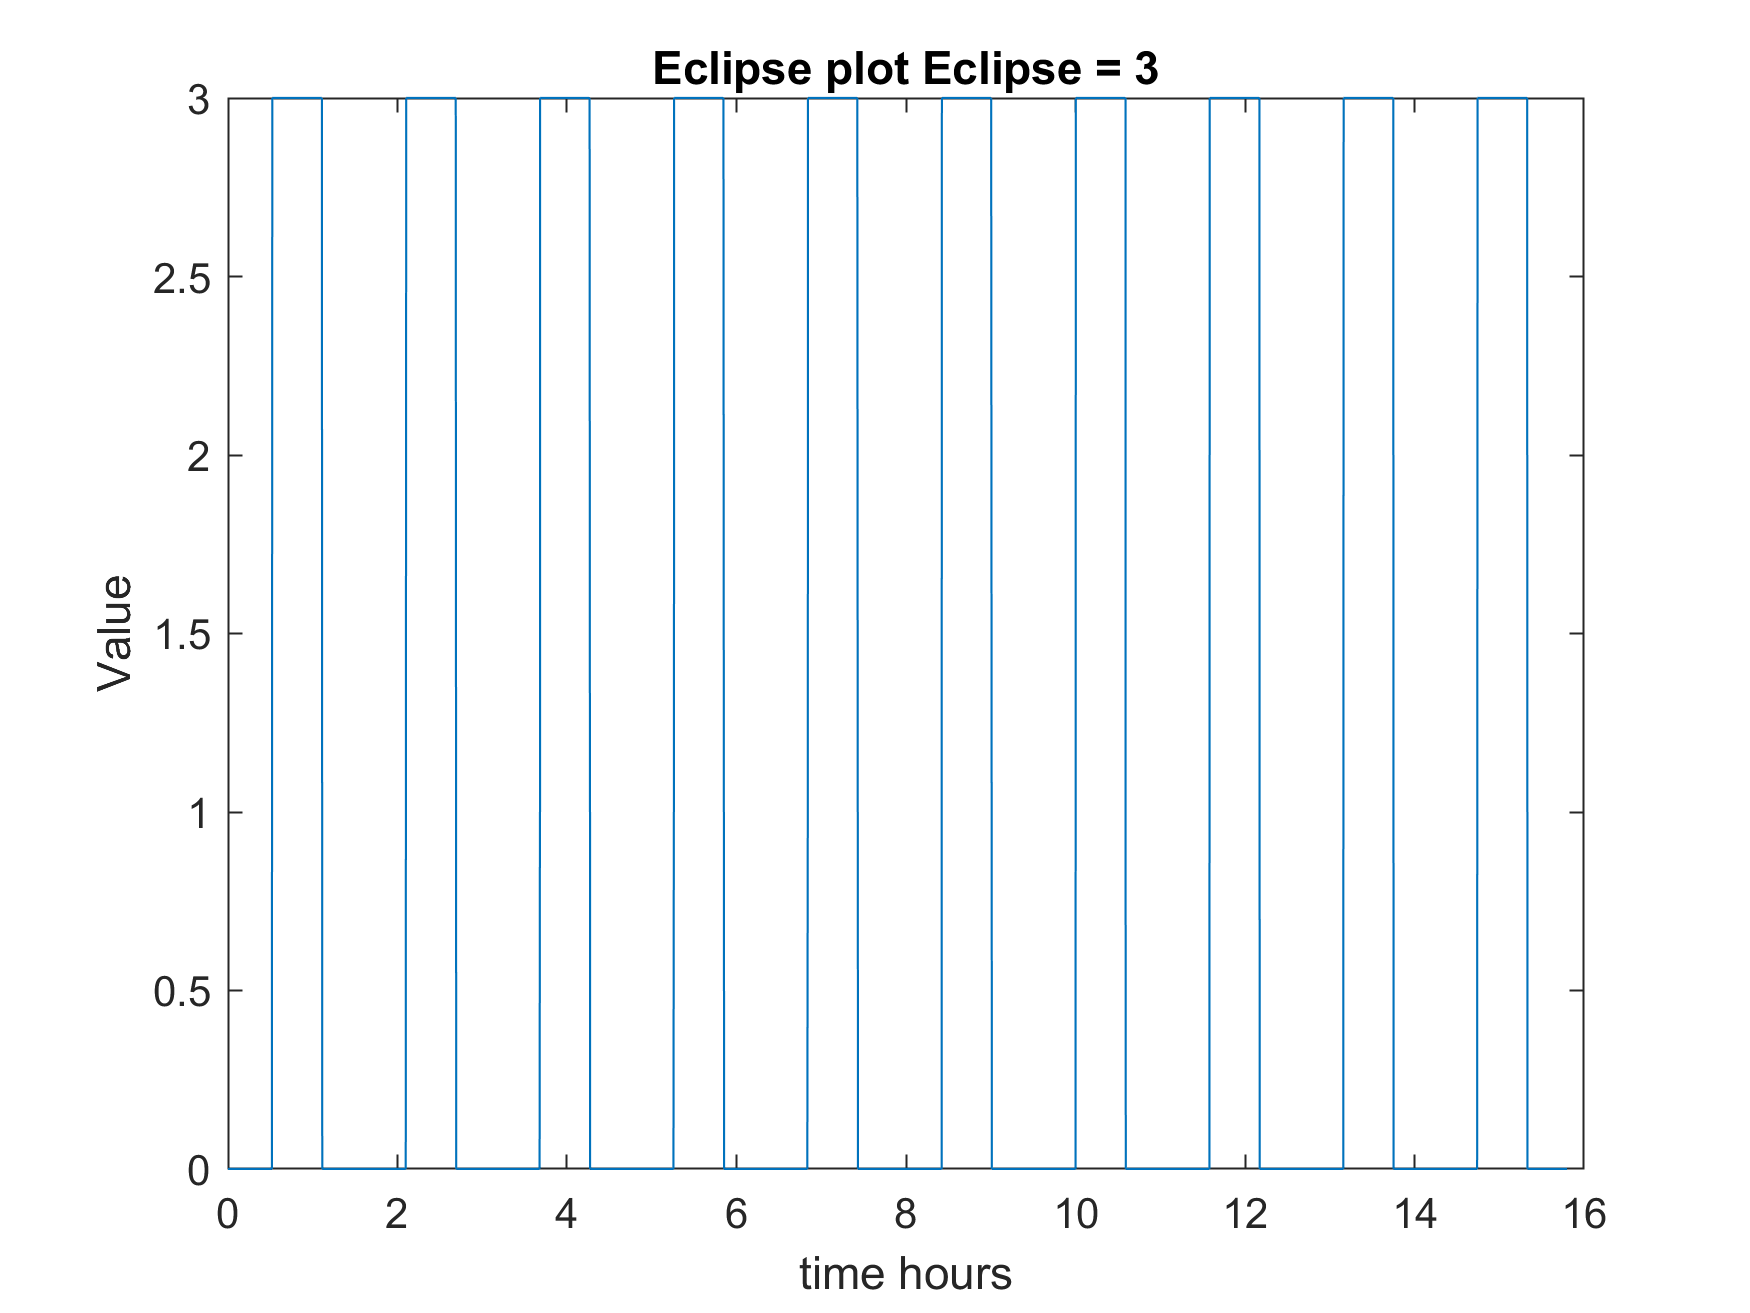
\includegraphics[width=0.7\linewidth]{res/img/Nadir_no_EKF/Eclipse phases.png}
            \caption{Eclipse phases}
            \label{fig:EclipsePhases}
        \end{figure}

    \end{itemize}

    \item \textbf{Number of simuated orbits:} 10 orbits
    \item \textbf{Simulation starting date:} 05/04/2027 00:00:00 UTC
    \item \textbf{Simulation time step:} 2 seconds
\end{itemize}

\subsubsection{Nadir pointing results}
\begin{itemize}
    \item \textbf{External perturbations}\\
    In the following plots, the values of the different external perturbations affecting
    the simulation are shown.
    \begin{figure}[H]
    \centering
    \begin{minipage}{0.48\linewidth}
        \centering
        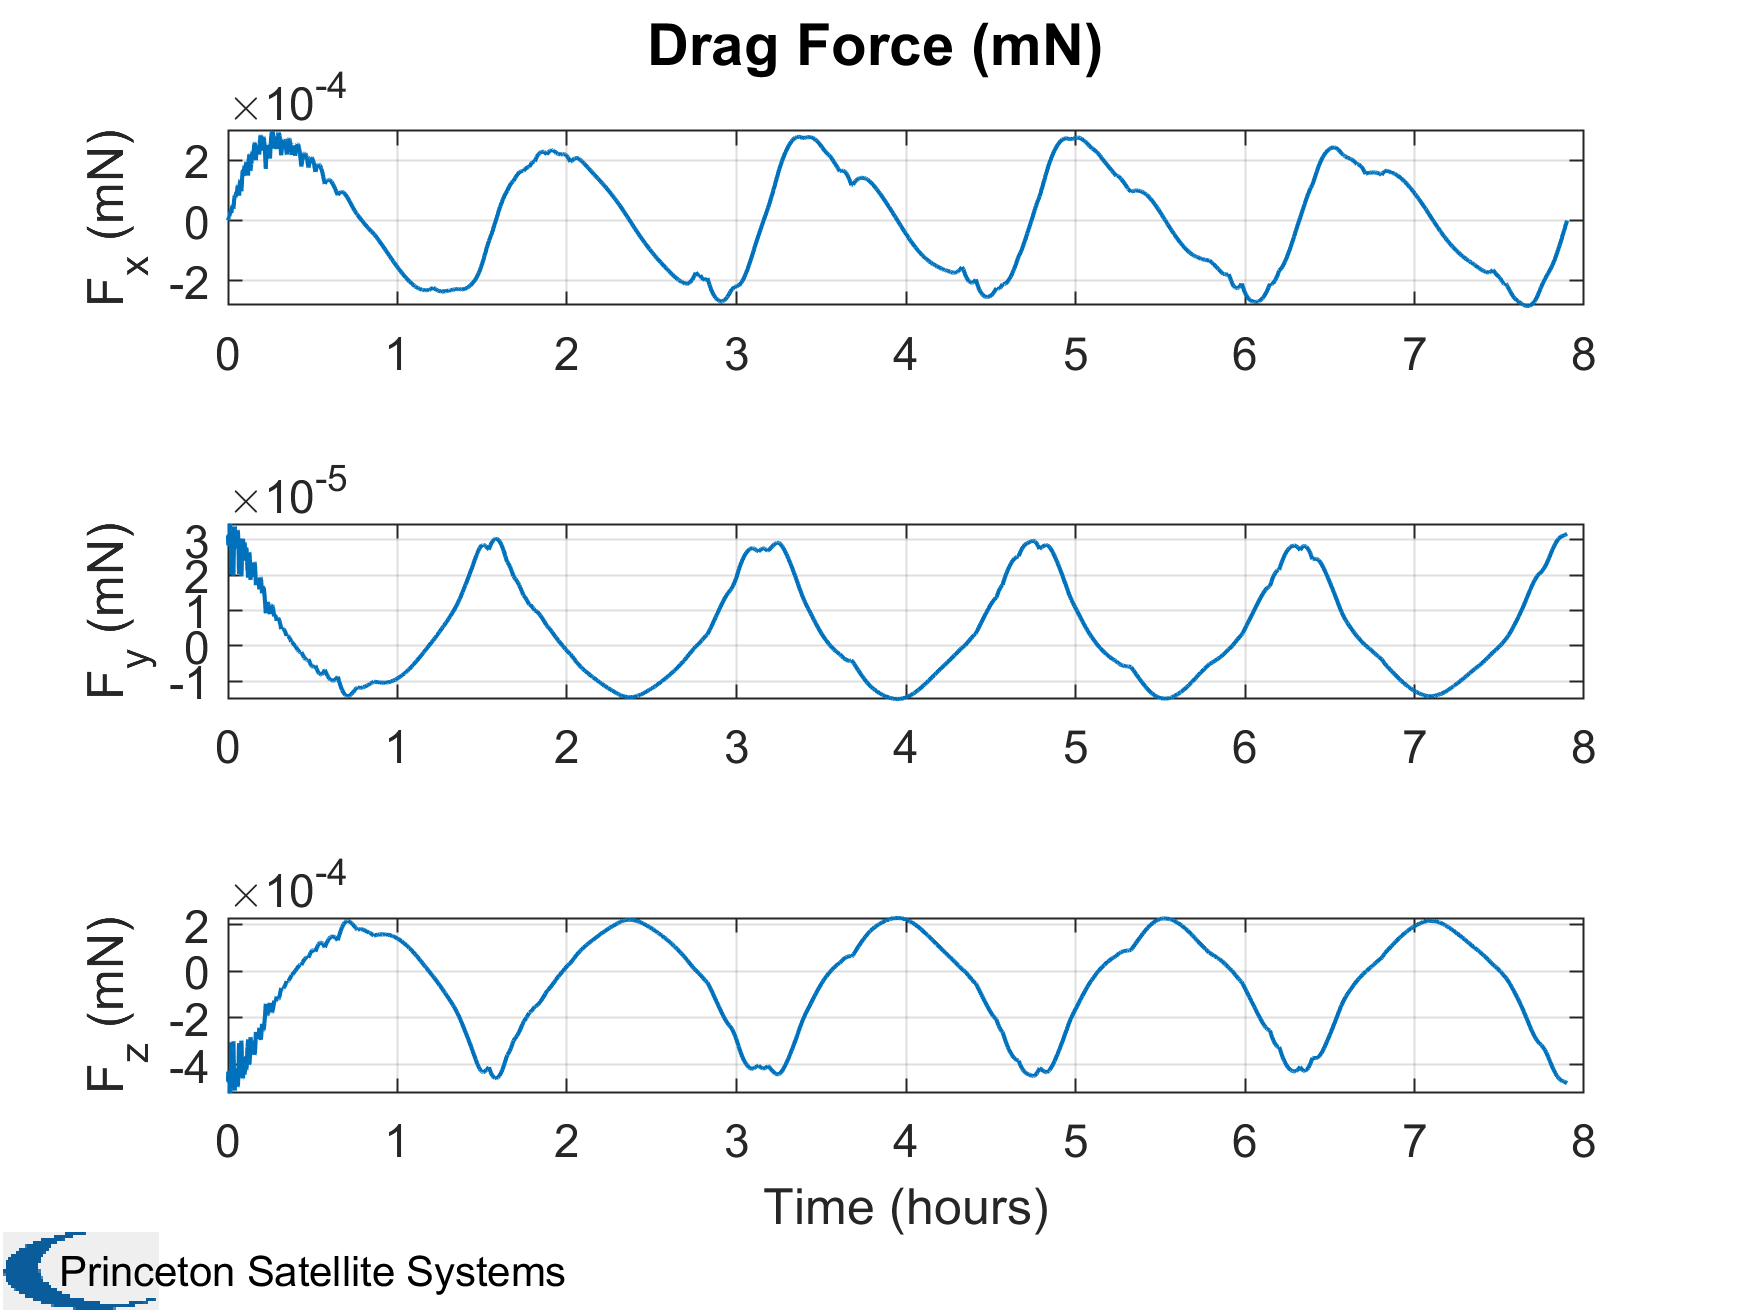
\includegraphics[width=0.95\linewidth]{res/img/Nadir_no_EKF/Drag Force (mN).png}
        \caption{Drag Force (mN)}
        \label{fig:DragForce}
    \end{minipage}\hfill
    \begin{minipage}{0.48\linewidth}
        \centering
        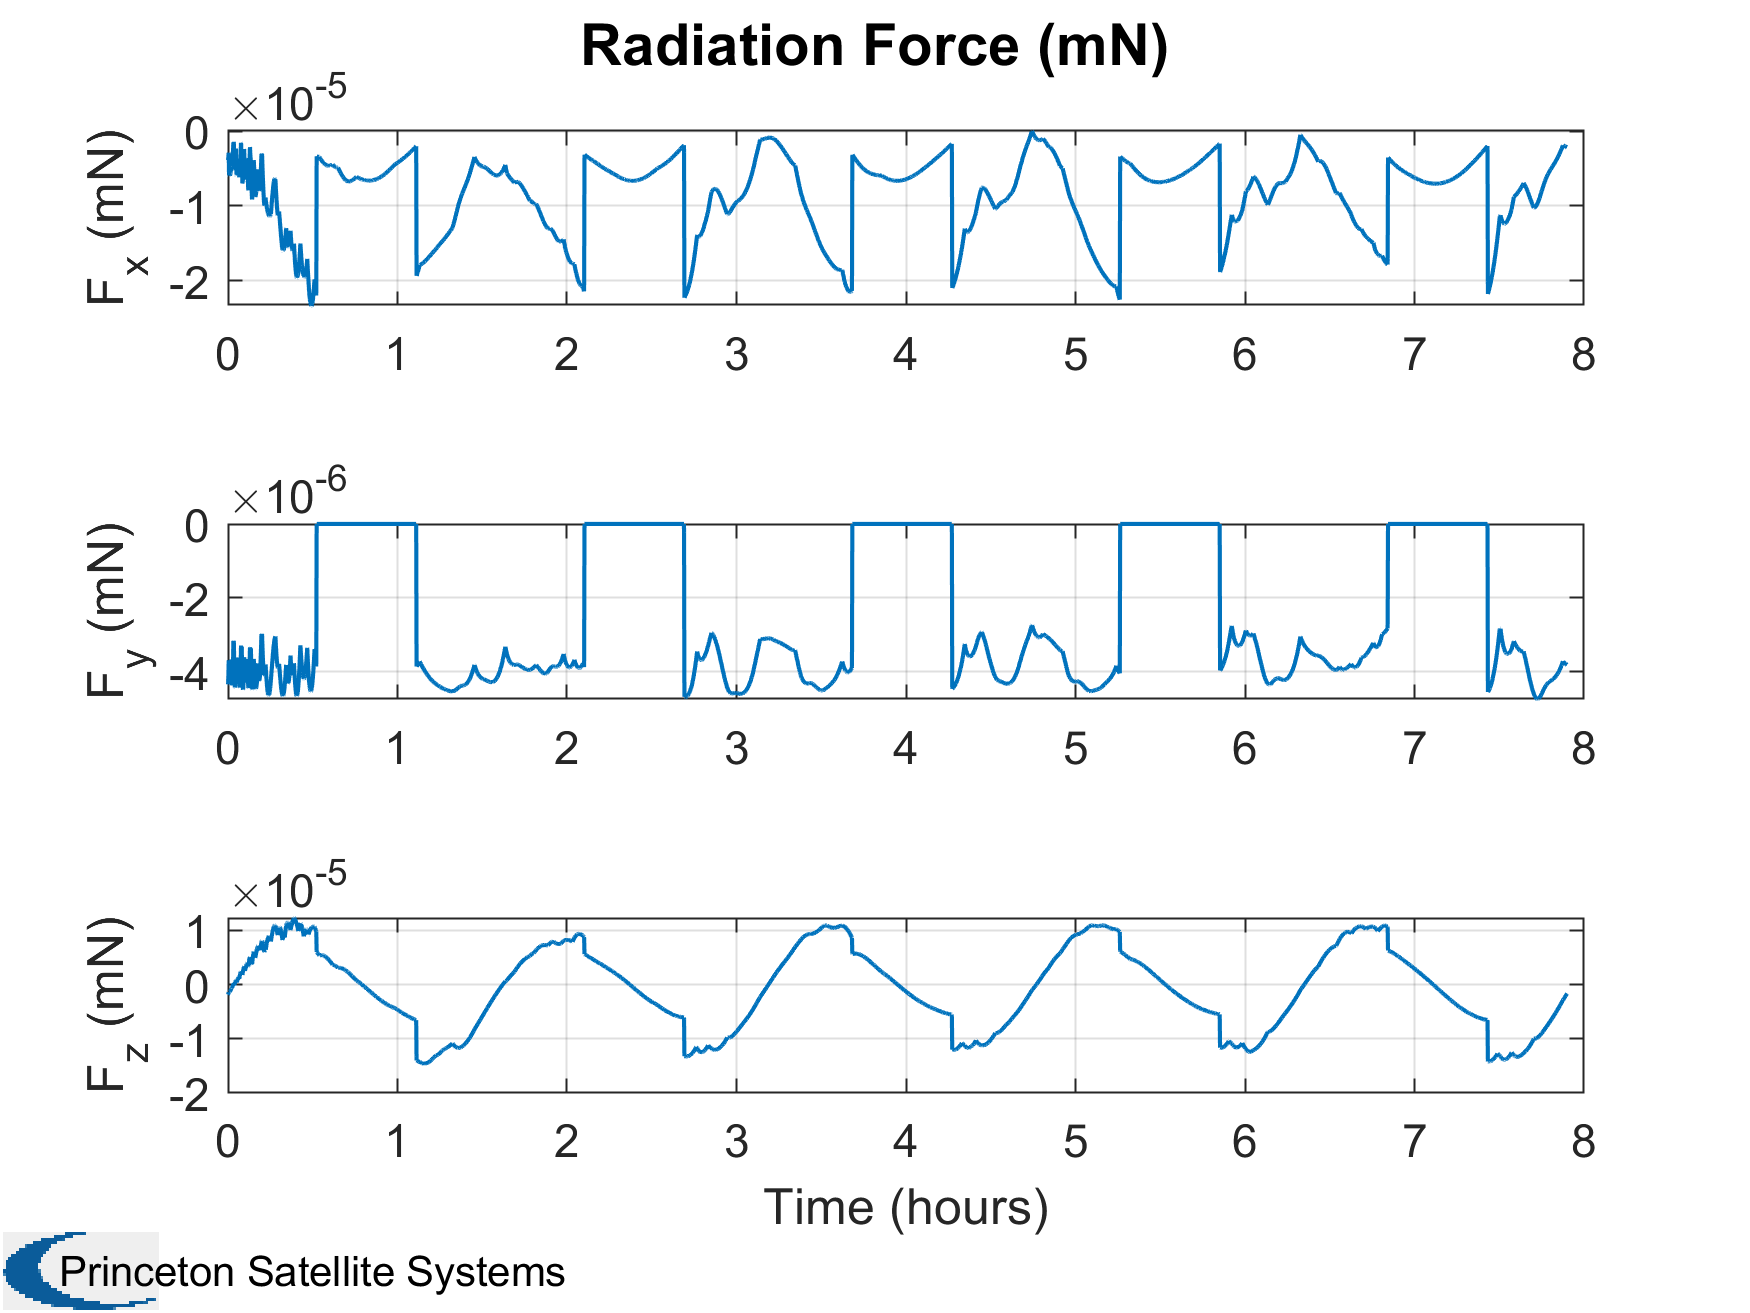
\includegraphics[width=0.95\linewidth]{res/img/Nadir_no_EKF/Radiation Force (mN).png}
        \caption{Radiation Force (mN)}
        \label{fig:RadiationForce}
    \end{minipage}
\end{figure}

\begin{figure}[H]
    \centering
    \begin{minipage}{0.48\linewidth}
        \centering
        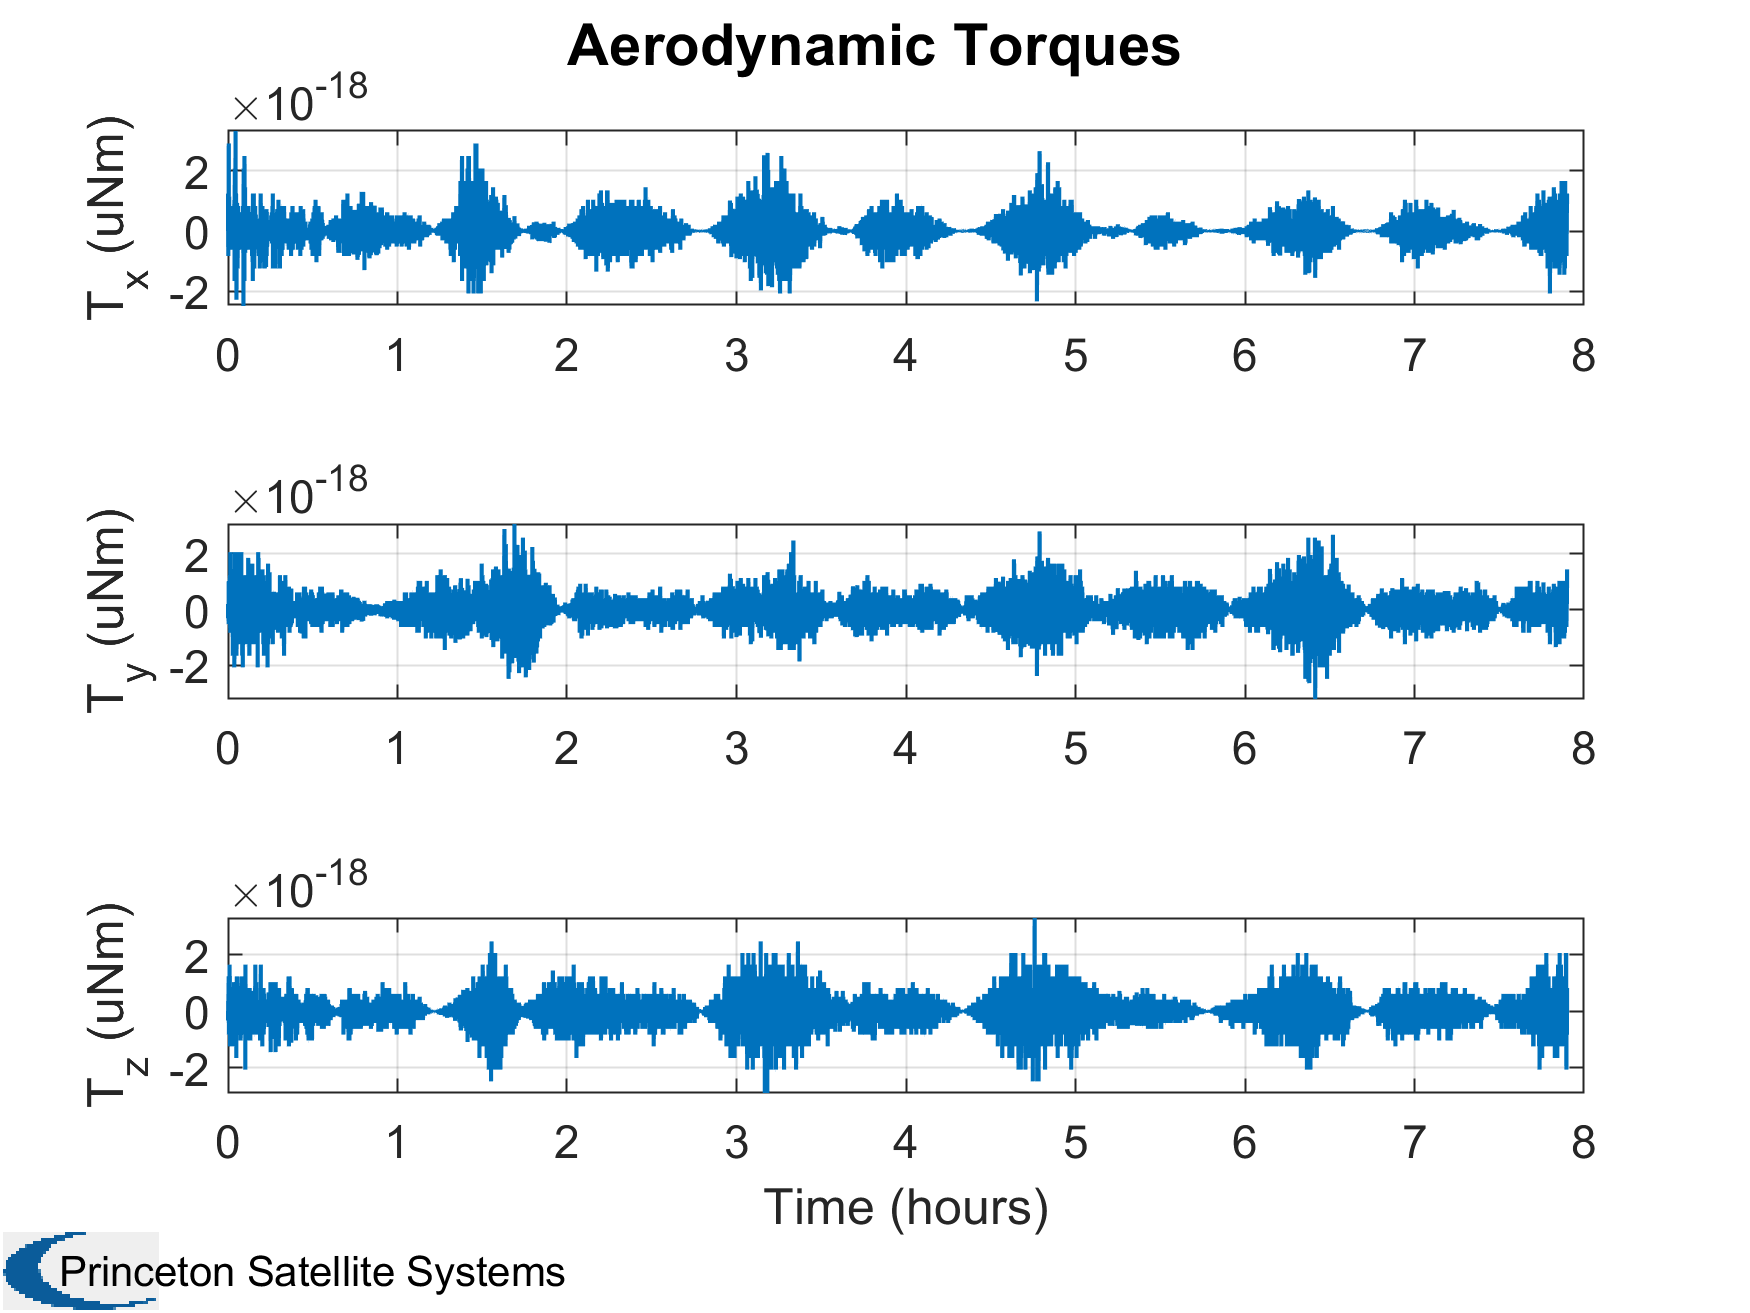
\includegraphics[width=0.95\linewidth]{res/img/Nadir_no_EKF/Aerodynamic Torques.png}
        \caption{Aerodynamic Torques}
        \label{fig:AerodynamicTorques}
    \end{minipage}\hfill
    \begin{minipage}{0.48\linewidth}
        \centering
        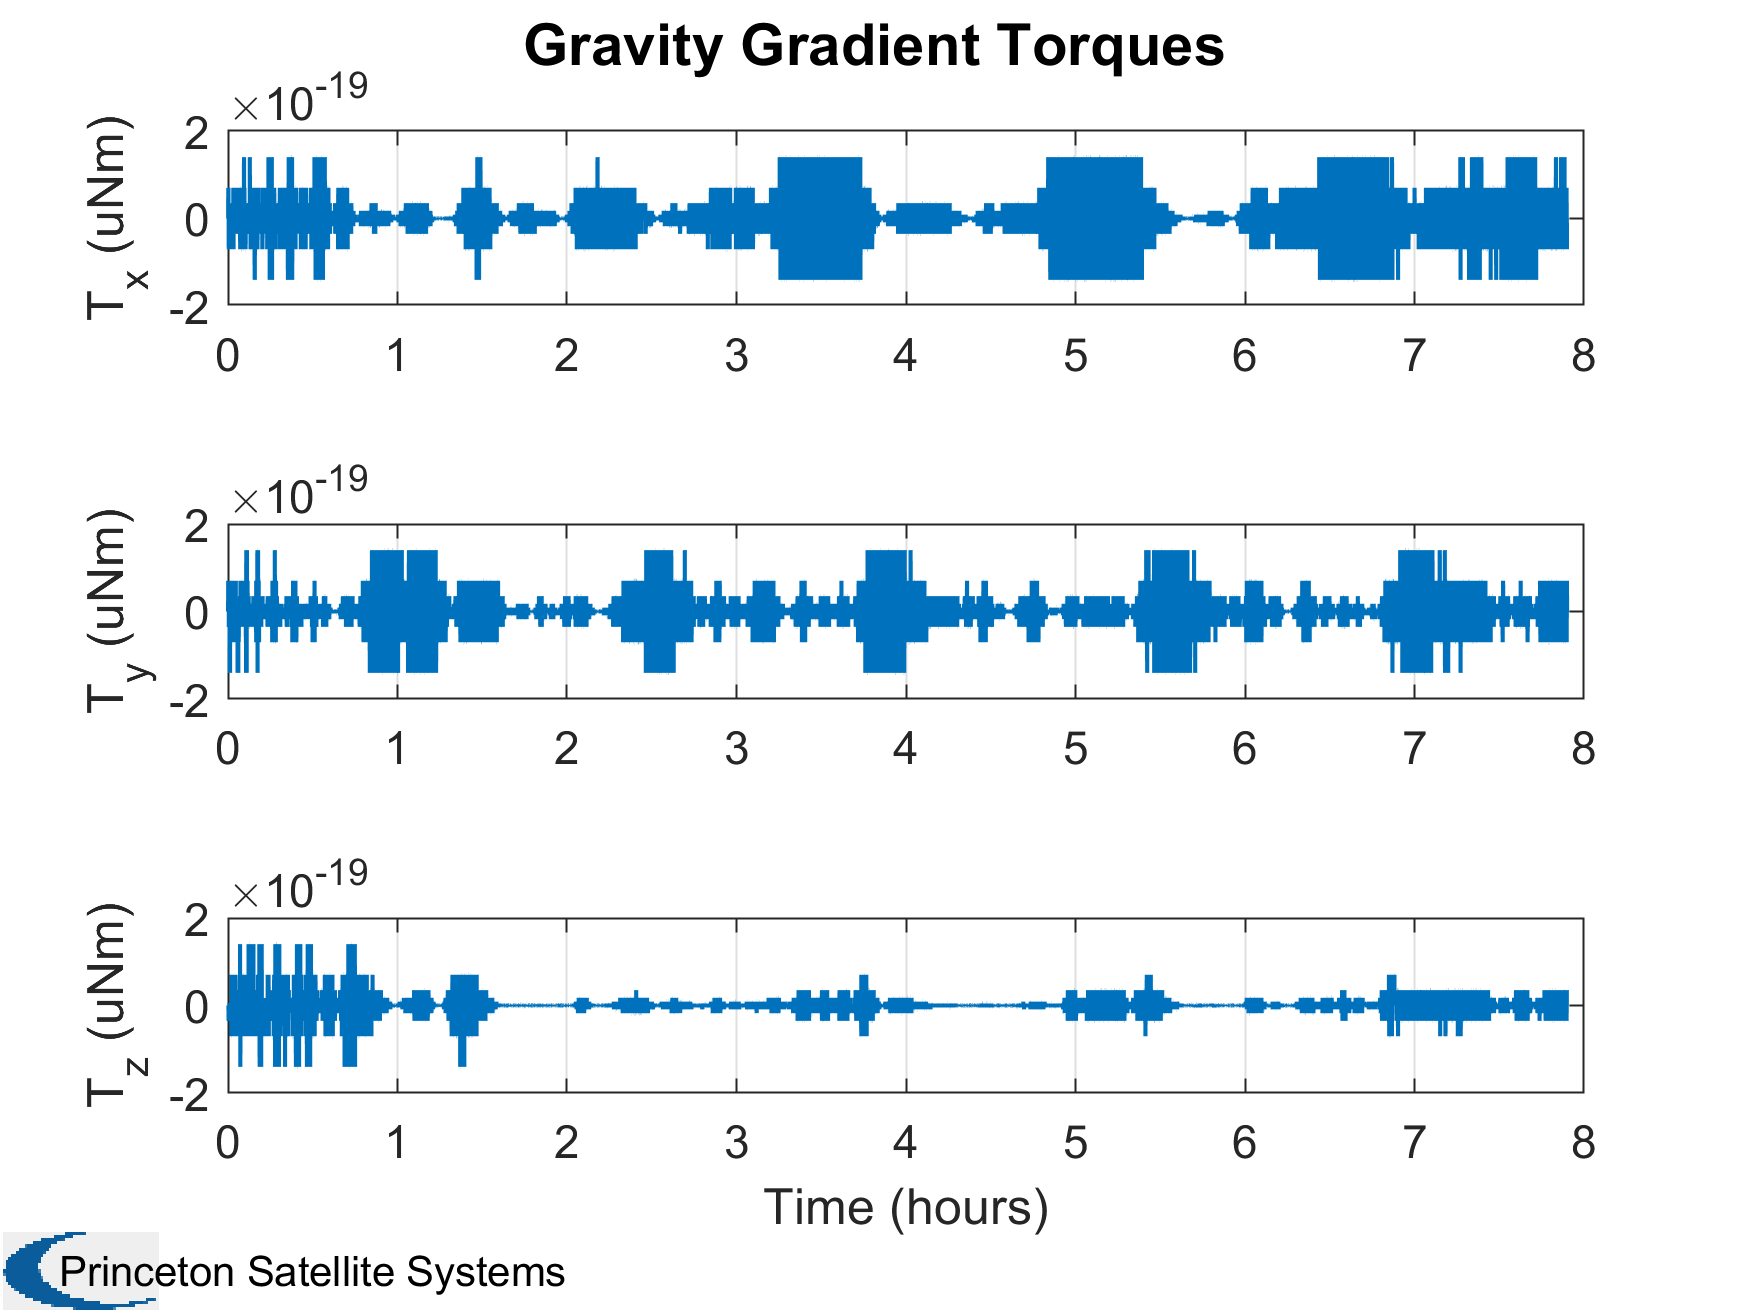
\includegraphics[width=0.95\linewidth]{res/img/Nadir_no_EKF/Gravity Gradient Torques.png}
        \caption{Gravity Gradient Torques}
        \label{fig:GravityGradientTorques}
    \end{minipage}
\end{figure}

\begin{figure}[H]
    \centering
    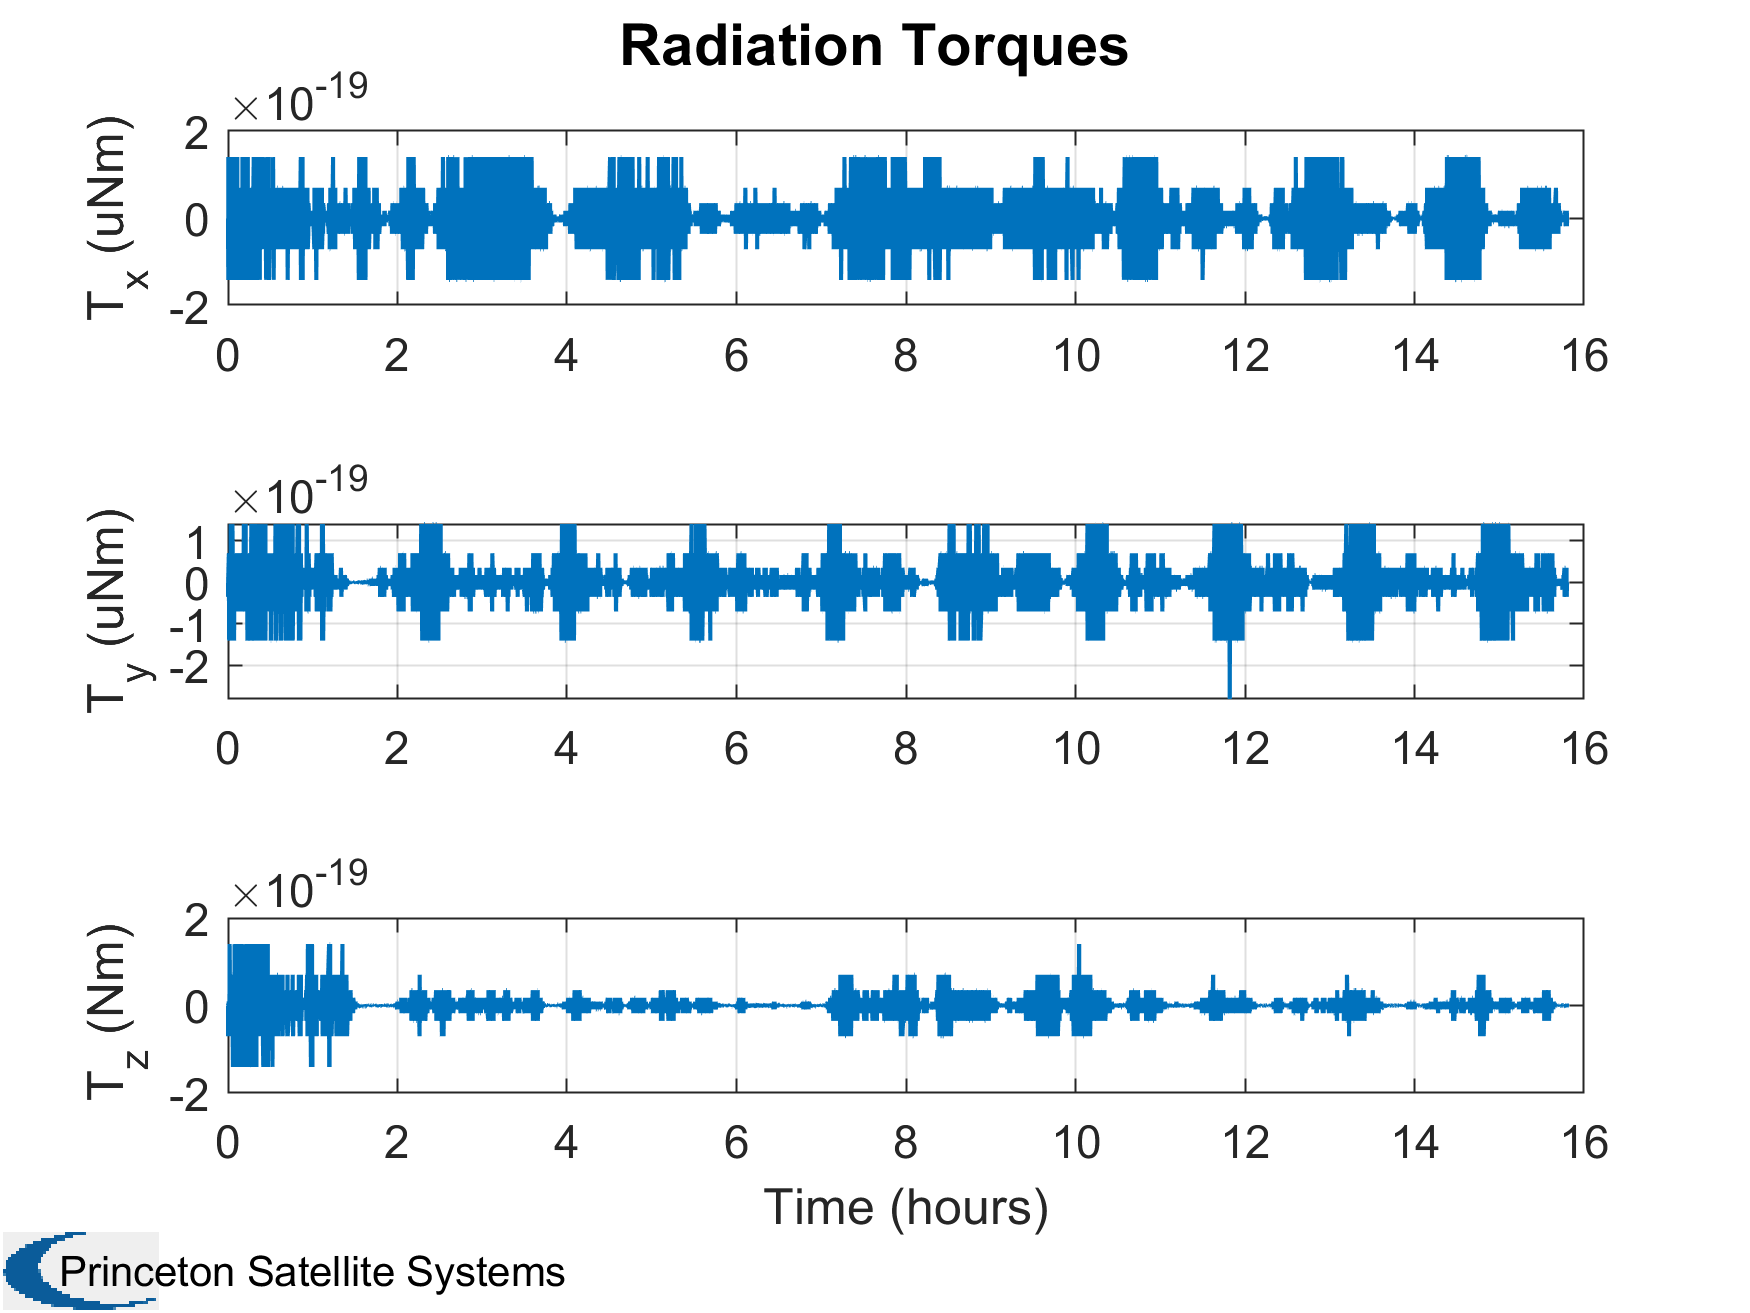
\includegraphics[width=0.48\linewidth]{res/img/Nadir_no_EKF/Radiation Torques.png}
    \caption{Radiation Torques}
    \label{fig:RadiationTorques}
\end{figure}

\begin{figure}[H]
    \centering
    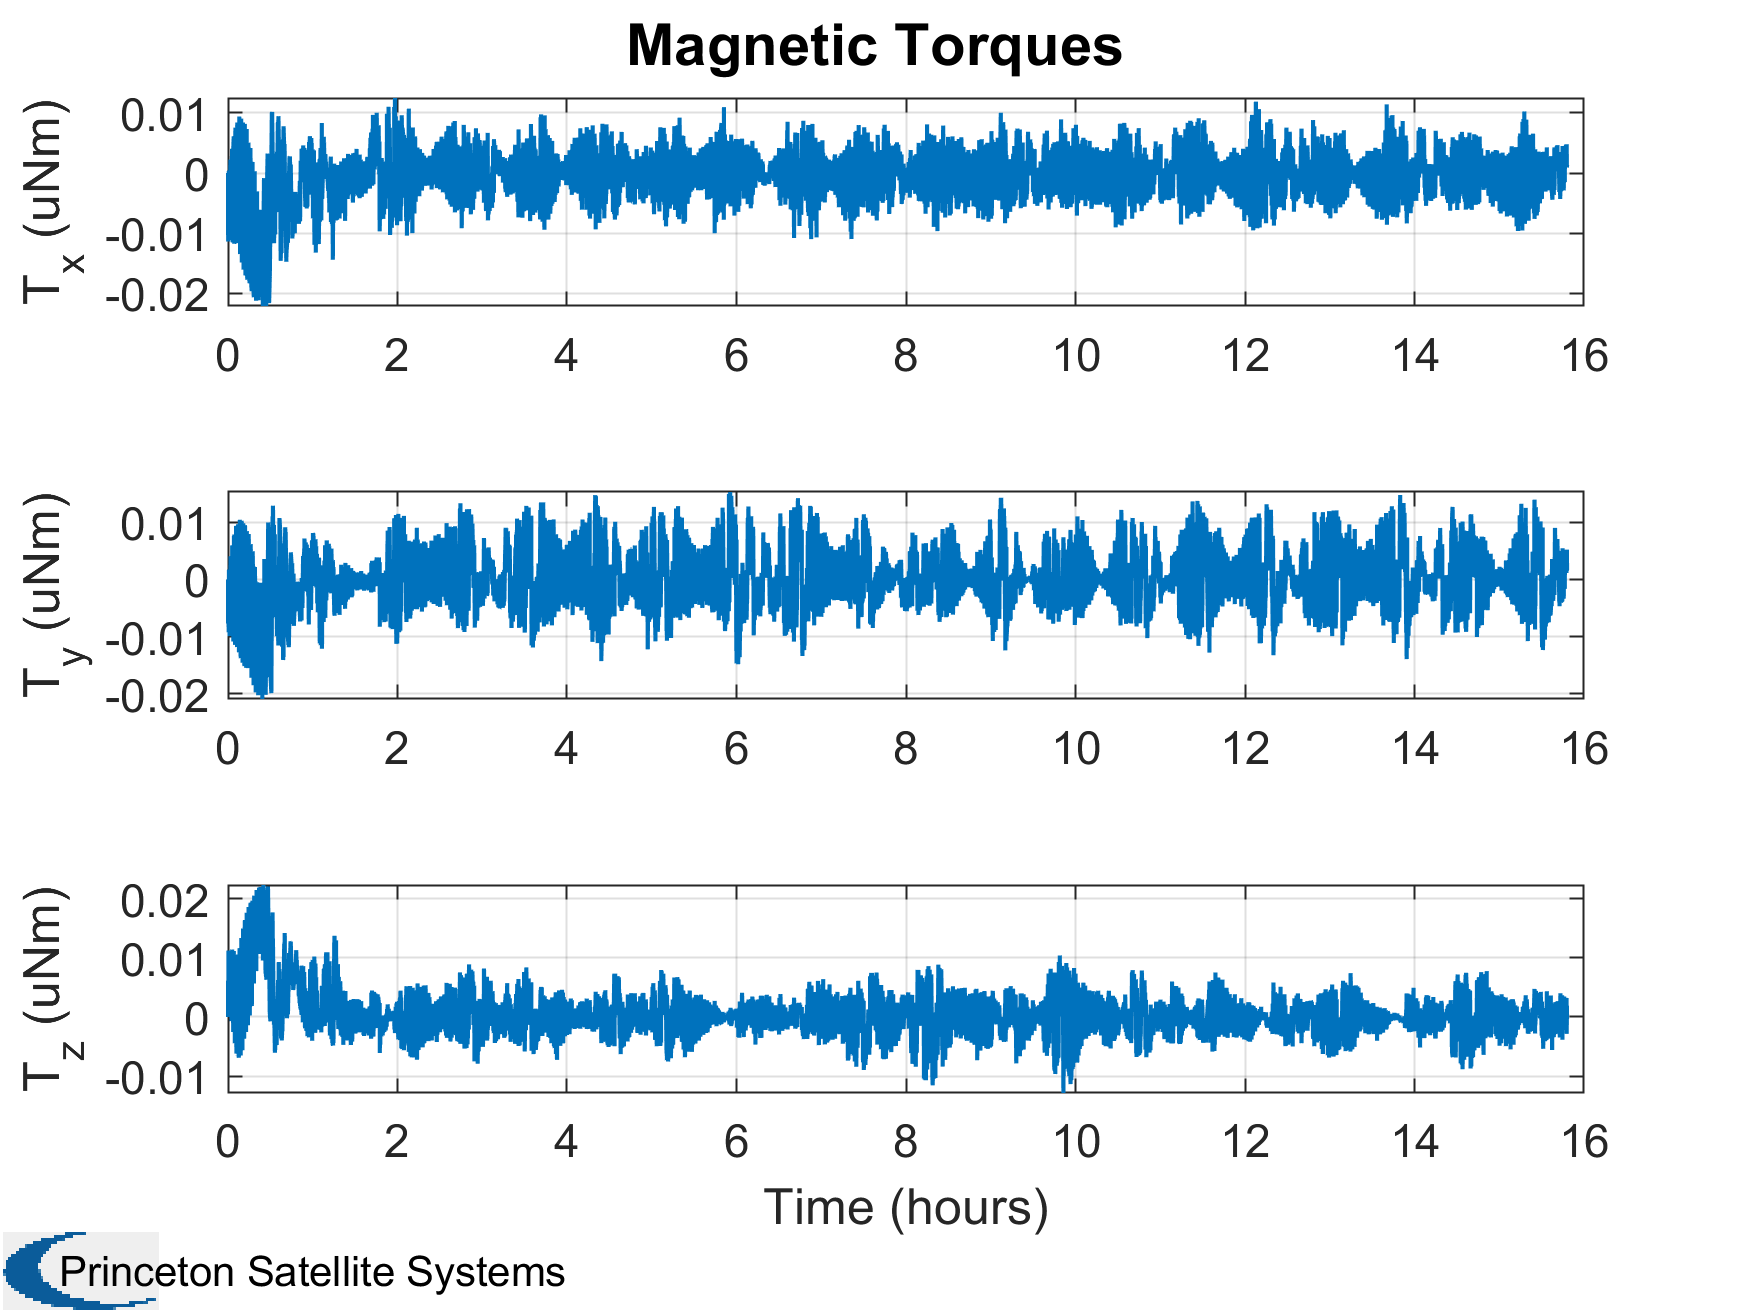
\includegraphics[width=0.48\linewidth]{res/img/Nadir_no_EKF/Magnetic Torques.png}
    \caption{Magnetic Torques}
    \label{fig:Magnetic torque}
\end{figure}

    \item \textbf{Sensor measurements}\\
    In this section the measures taken from the simulated sensors are presented. The sensors
    follow the model presented in the previous sections of the document. Firstly the measurements
    of the gyroscope are presented, it can be observed the effect that the noise and the random walk
    phenomenon has on the measures. It can also be observed how the Nadir Pointing controller first tries to 
    conduct a little detumbling functionality in order to reduce the angular velocity ass much as possible. This
    effect can be observed in the first hour of the simulation.

    \begin{figure}[H]
        \centering
        \begin{minipage}{0.32\linewidth}
            \centering
            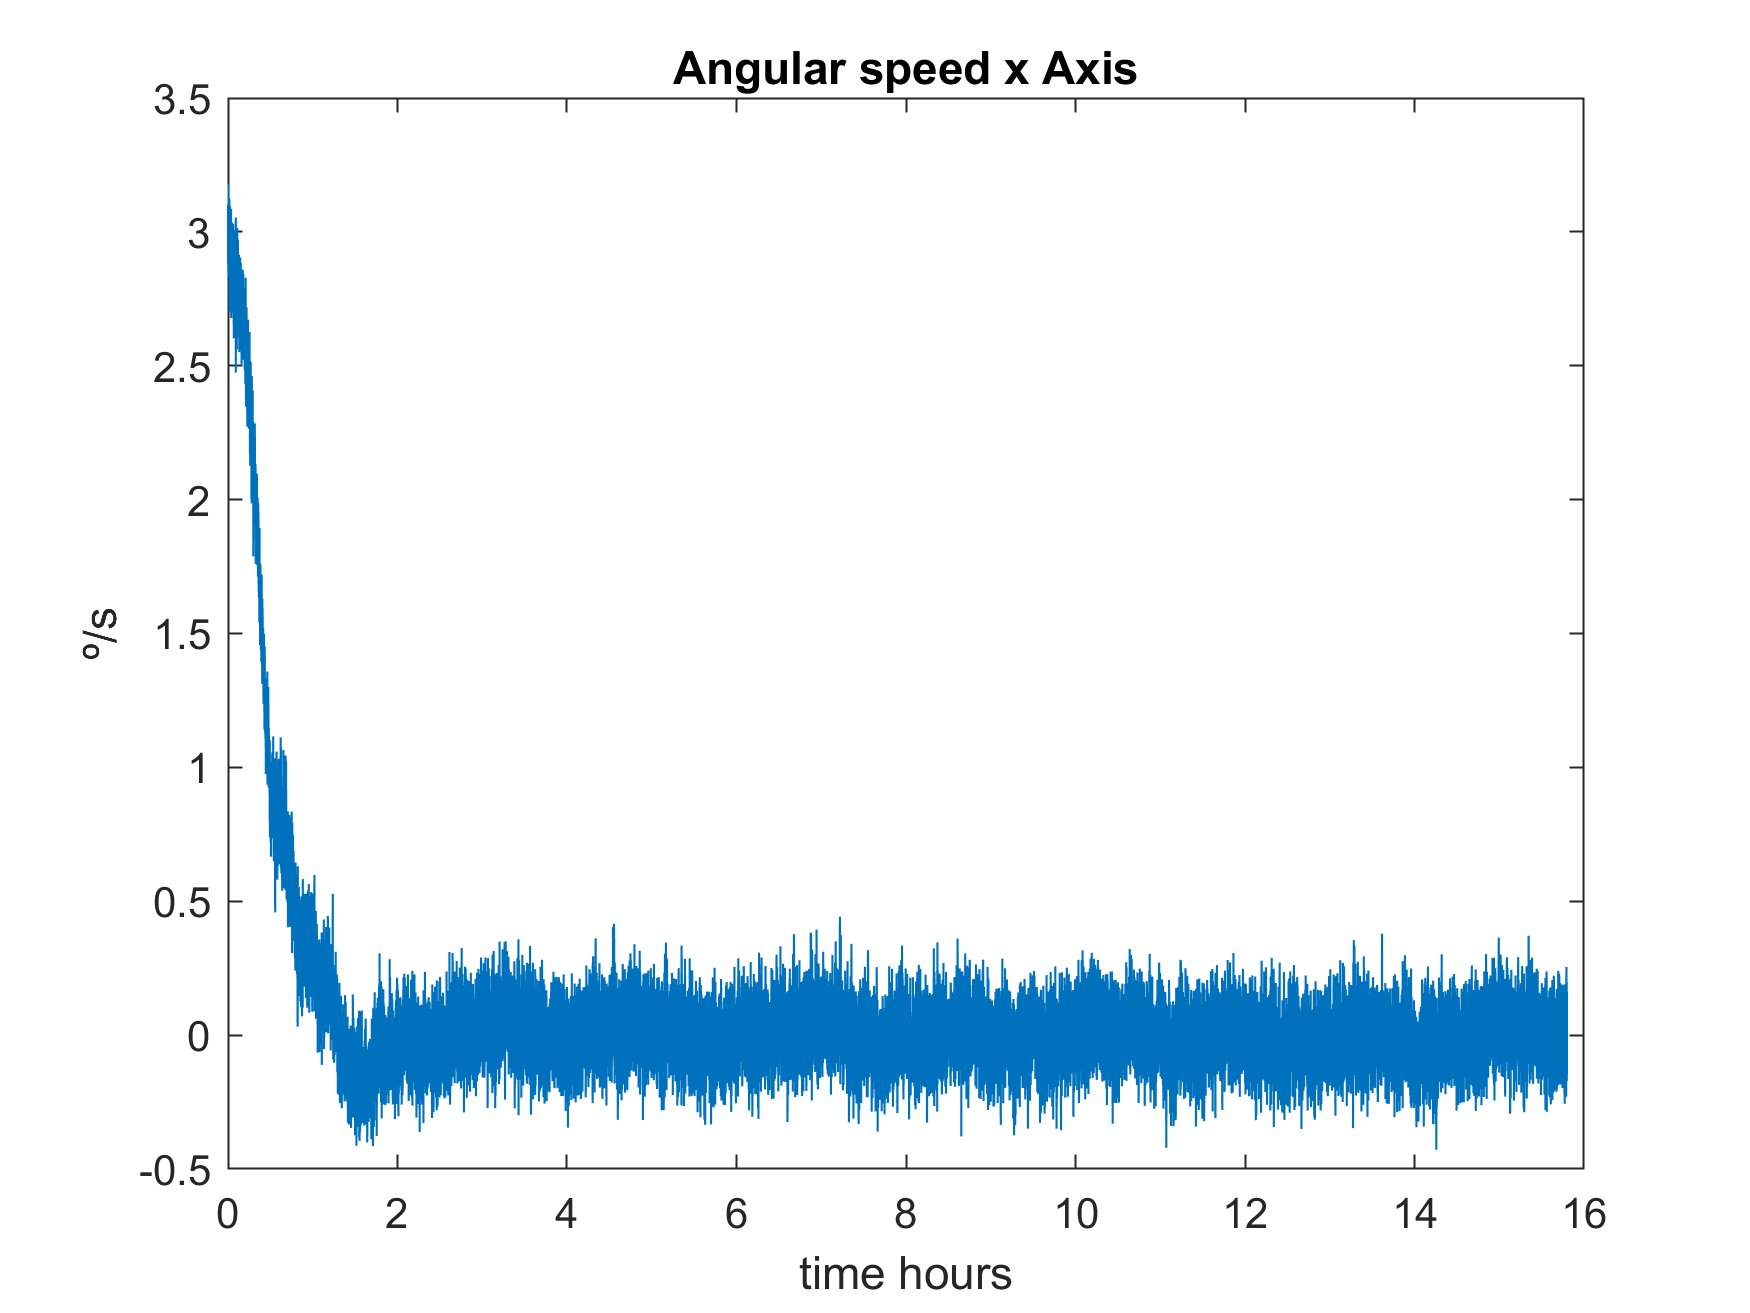
\includegraphics[width=0.95\linewidth]{res/img/Nadir_no_EKF/Gyro data X Axis.png}
            \caption{Gyro data X Axis}
            \label{fig:GyroDataX}
        \end{minipage}\hfill
        \begin{minipage}{0.32\linewidth}
            \centering
            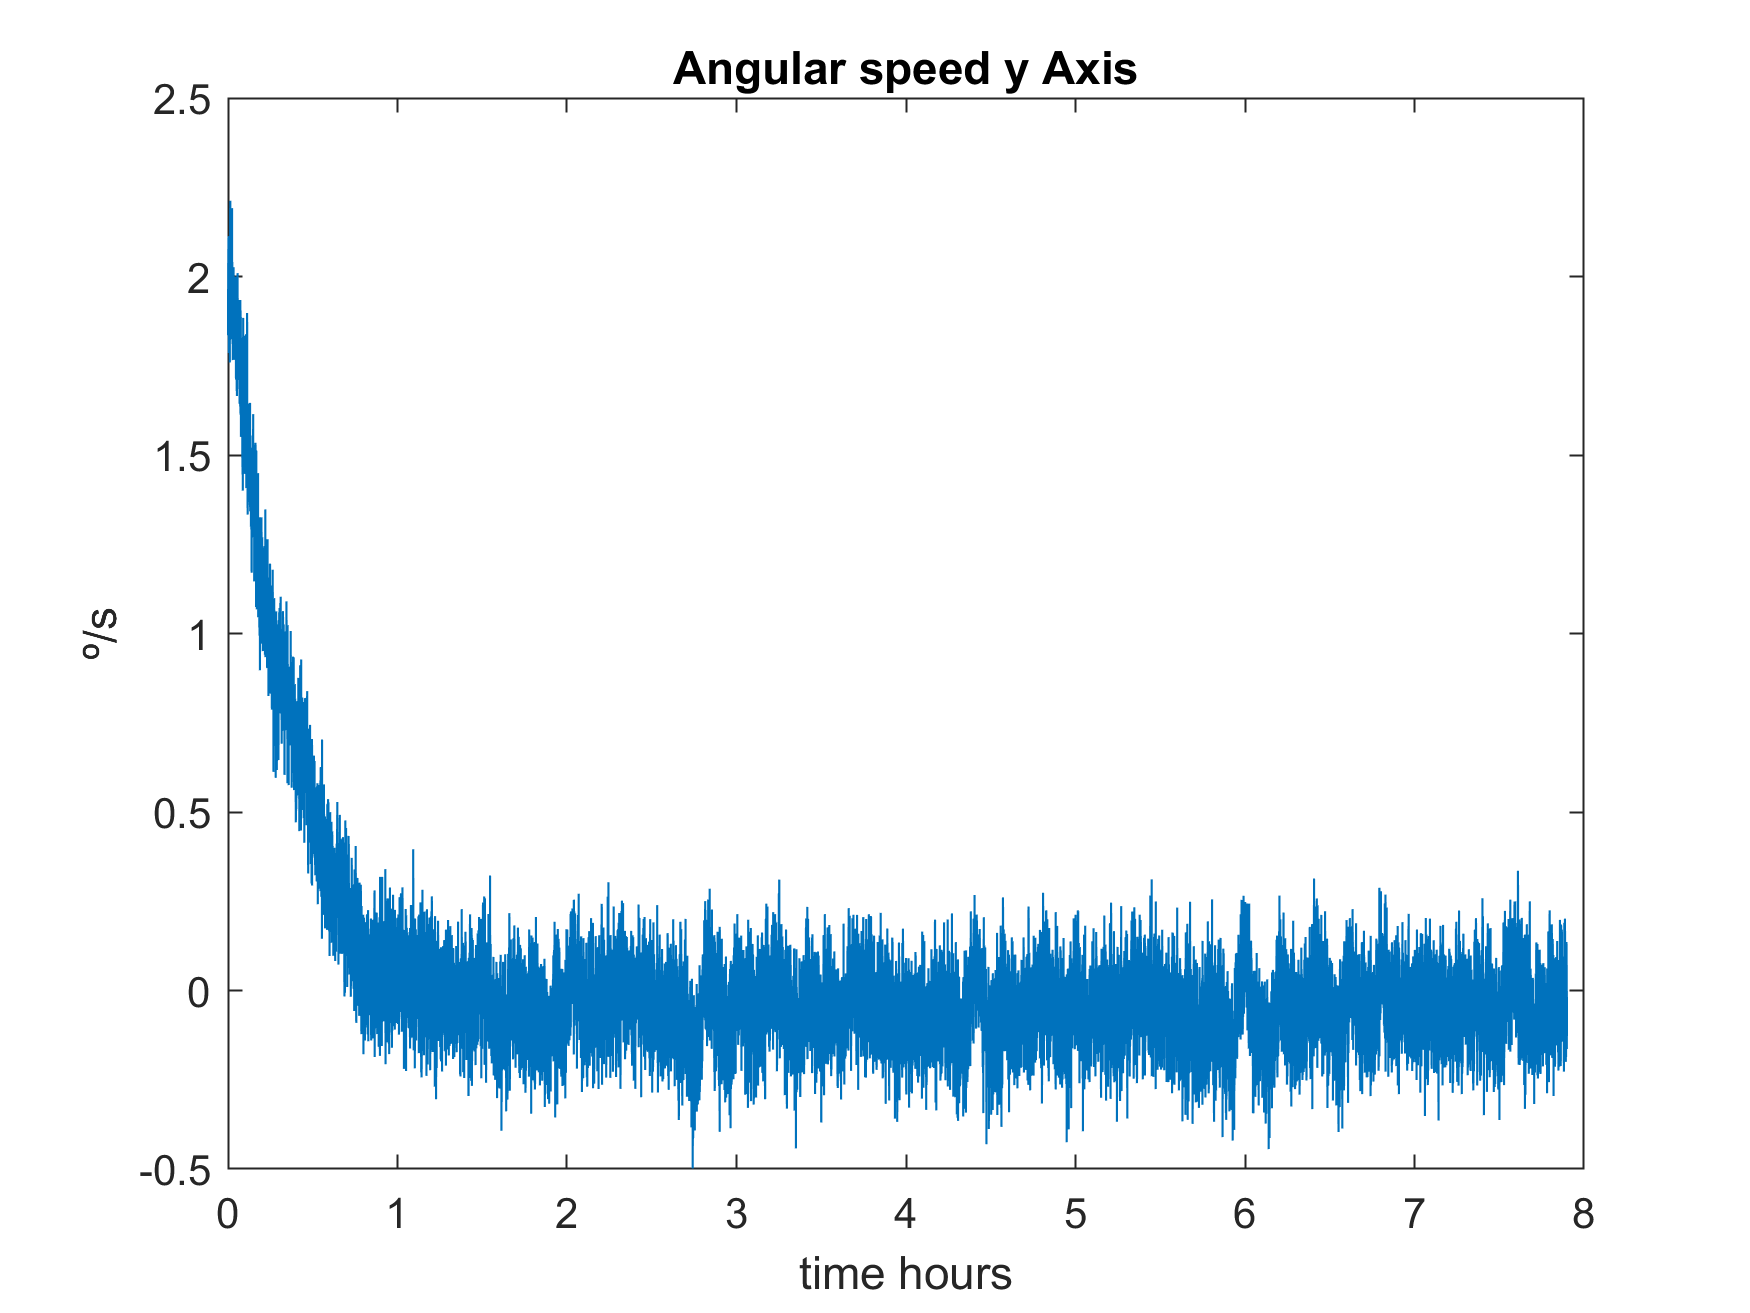
\includegraphics[width=0.95\linewidth]{res/img/Nadir_no_EKF/Gyro data Y Axis.png}
            \caption{Gyro data Y Axis}
            \label{fig:GyroDataY}
        \end{minipage}\hfill
        \begin{minipage}{0.32\linewidth}
            \centering
            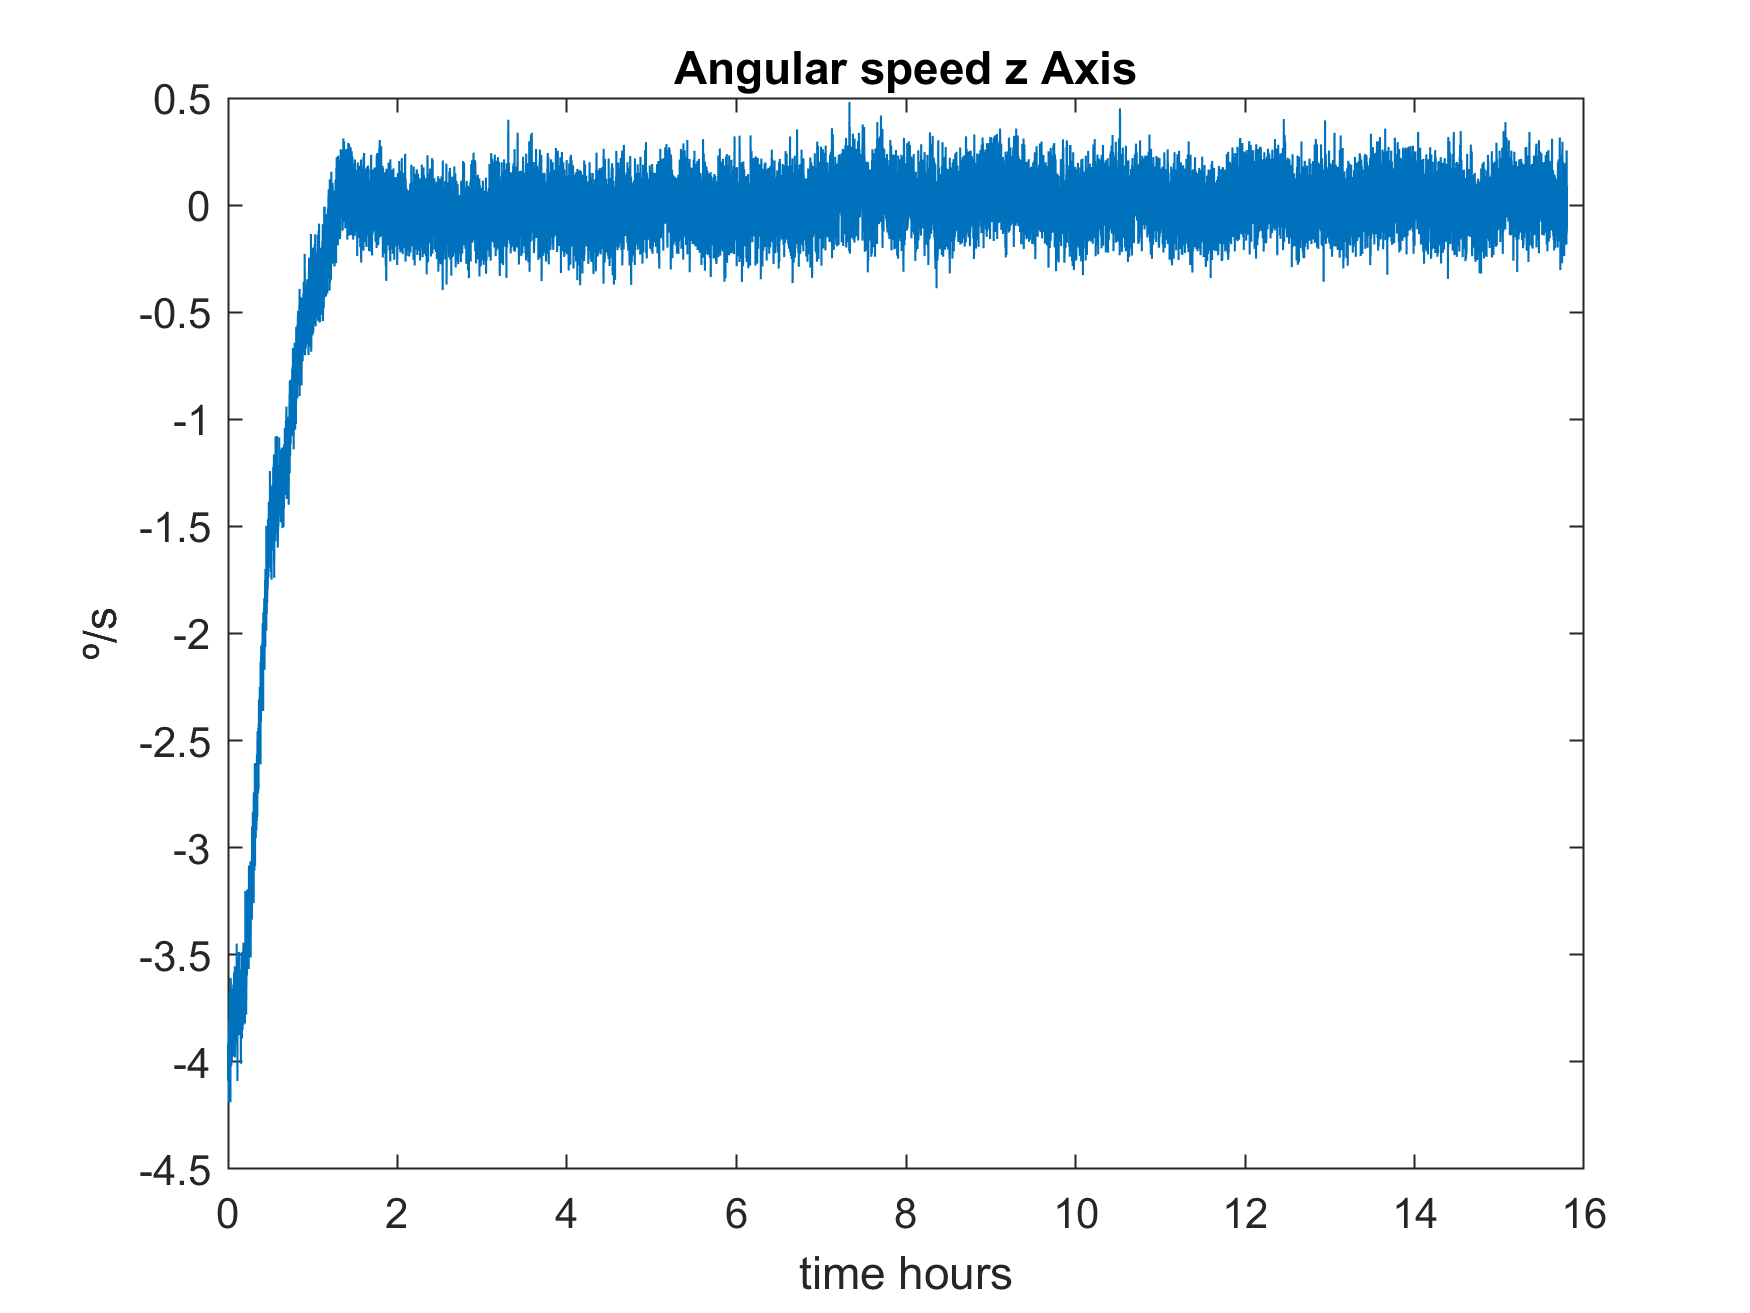
\includegraphics[width=0.95\linewidth]{res/img/Nadir_no_EKF/Gyro data Z Axis.png}
            \caption{Gyro data Z Axis}
            \label{fig:GyroDataZ}
        \end{minipage}
    \end{figure}

    Secondly, in the following pictures the magnetic field measured by the magnetometer is shown.
    \begin{figure}[H]
        \centering
        \begin{minipage}{0.32\linewidth}
            \centering
            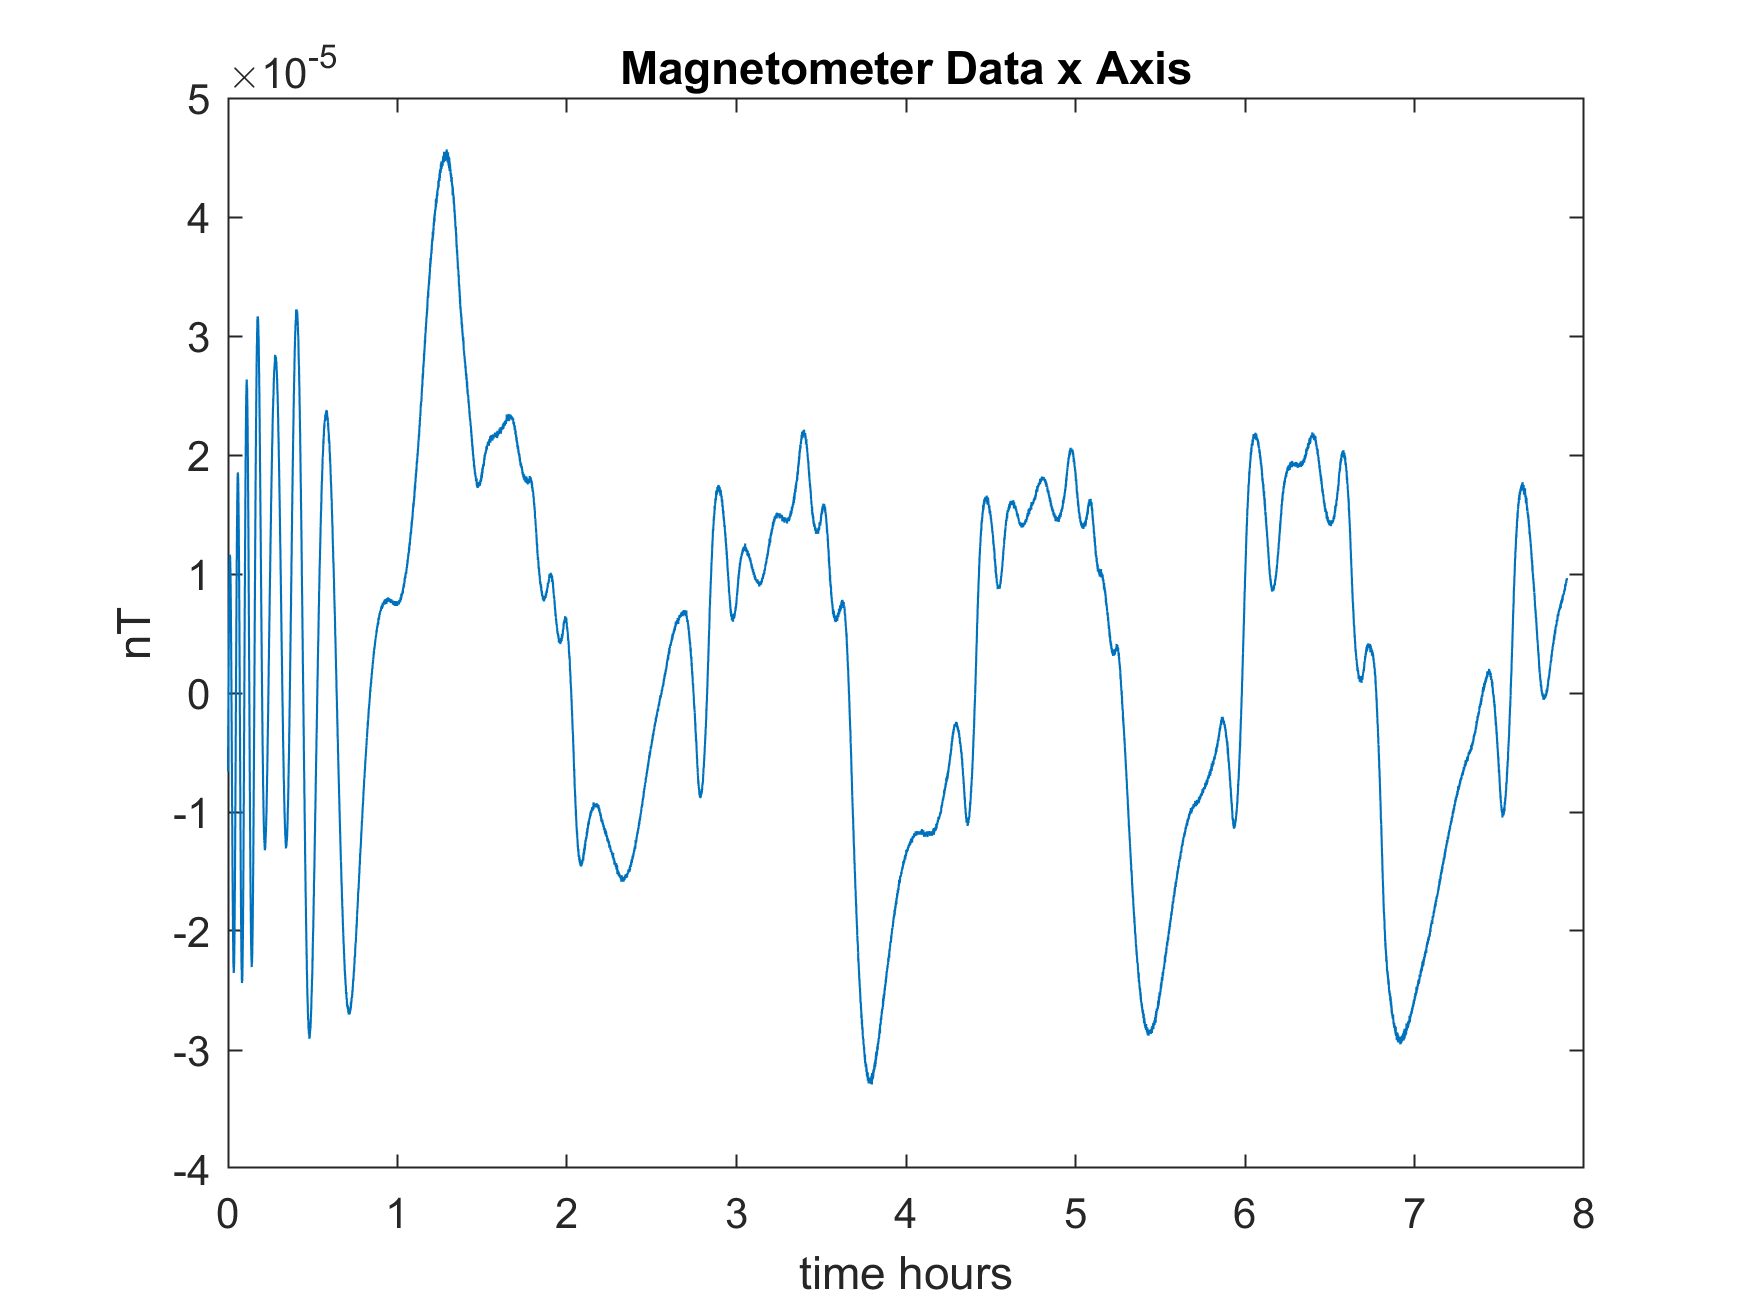
\includegraphics[width=0.95\linewidth]{res/img/Nadir_no_EKF/Magnetometer data X Axis.png}
            \caption{Magnetometer data X Axis}
            \label{fig:MagnetometerDataX}
        \end{minipage}\hfill
        \begin{minipage}{0.32\linewidth}
            \centering
            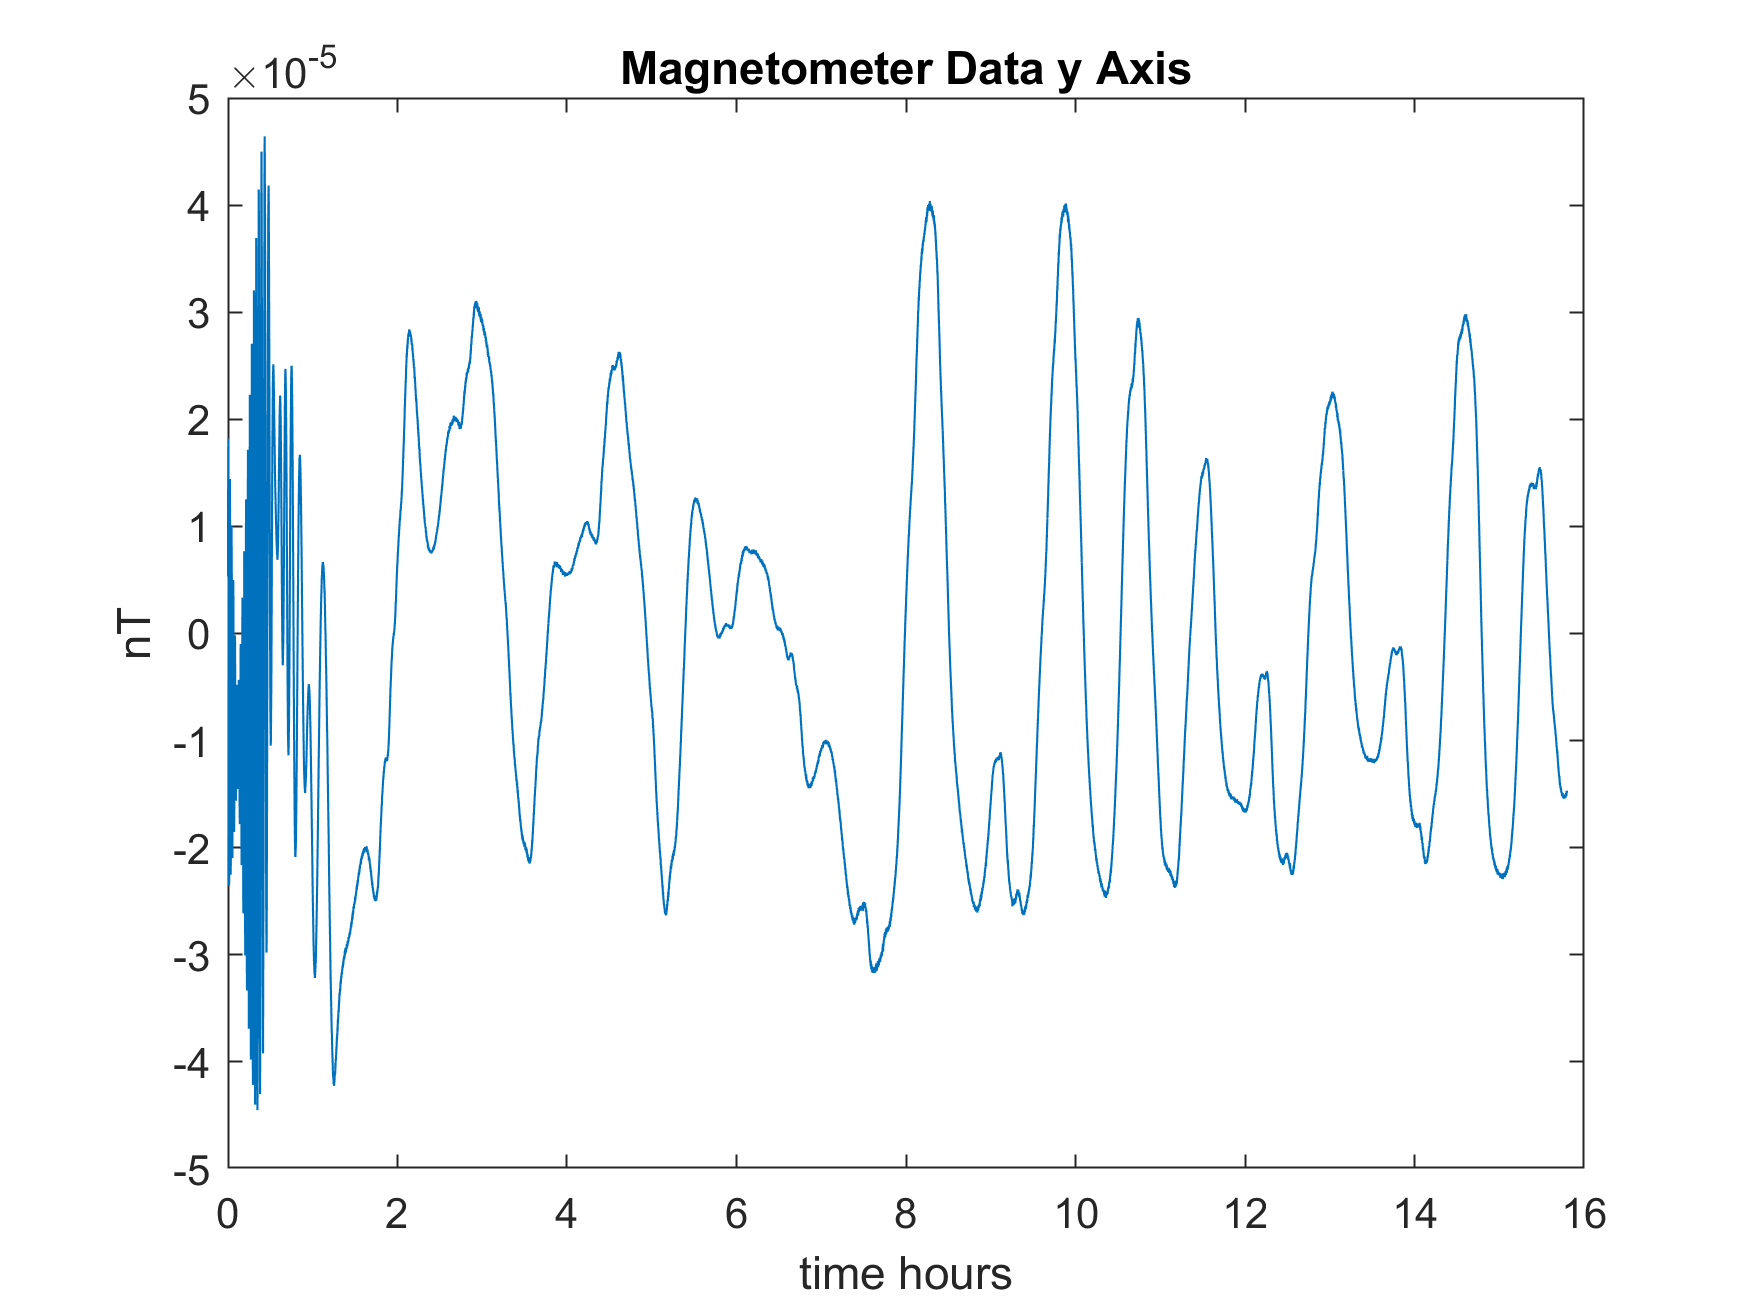
\includegraphics[width=0.95\linewidth]{res/img/Nadir_no_EKF/Magnetometer data Y Axis.png}
            \caption{Magnetometer data Y Axis}
            \label{fig:MagnetometerDataY}
        \end{minipage}\hfill
        \begin{minipage}{0.32\linewidth}
            \centering
            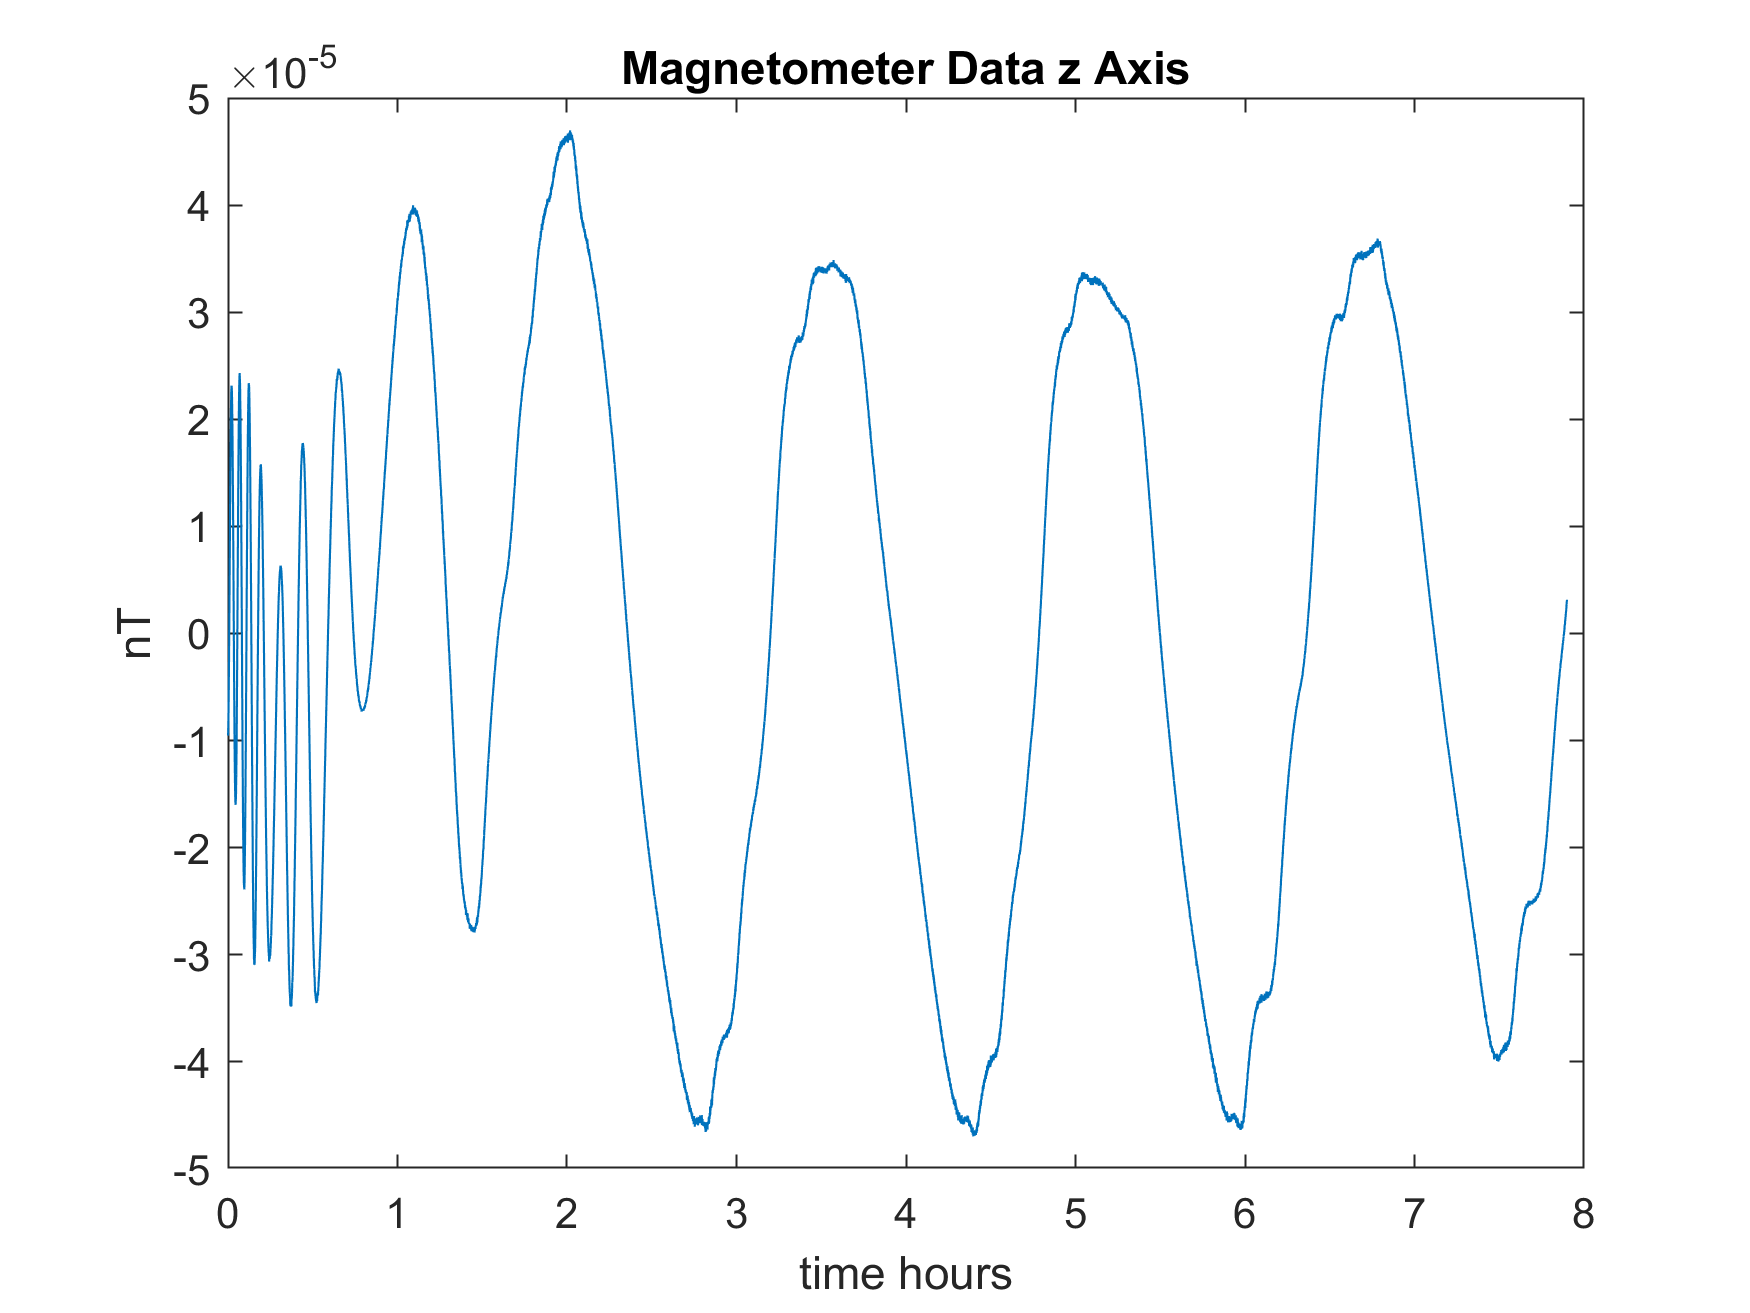
\includegraphics[width=0.95\linewidth]{res/img/Nadir_no_EKF/Magnetometer data Z Axis.png}
            \caption{Magnetometer data Z Axis}
            \label{fig:MagnetometerDataZ}
        \end{minipage}
    \end{figure}

    Finally, the last plot of the sensors includes the measurements of all 6 photodiodes used in the satellite. 
    Each axis of the PQ corresponds to the following number: 1 to +Z, 2 to -Z, 3 to +X, 4 to +Y,
    5 to -X and 6 to -Y.
    \begin{figure}[H]
        \centering
        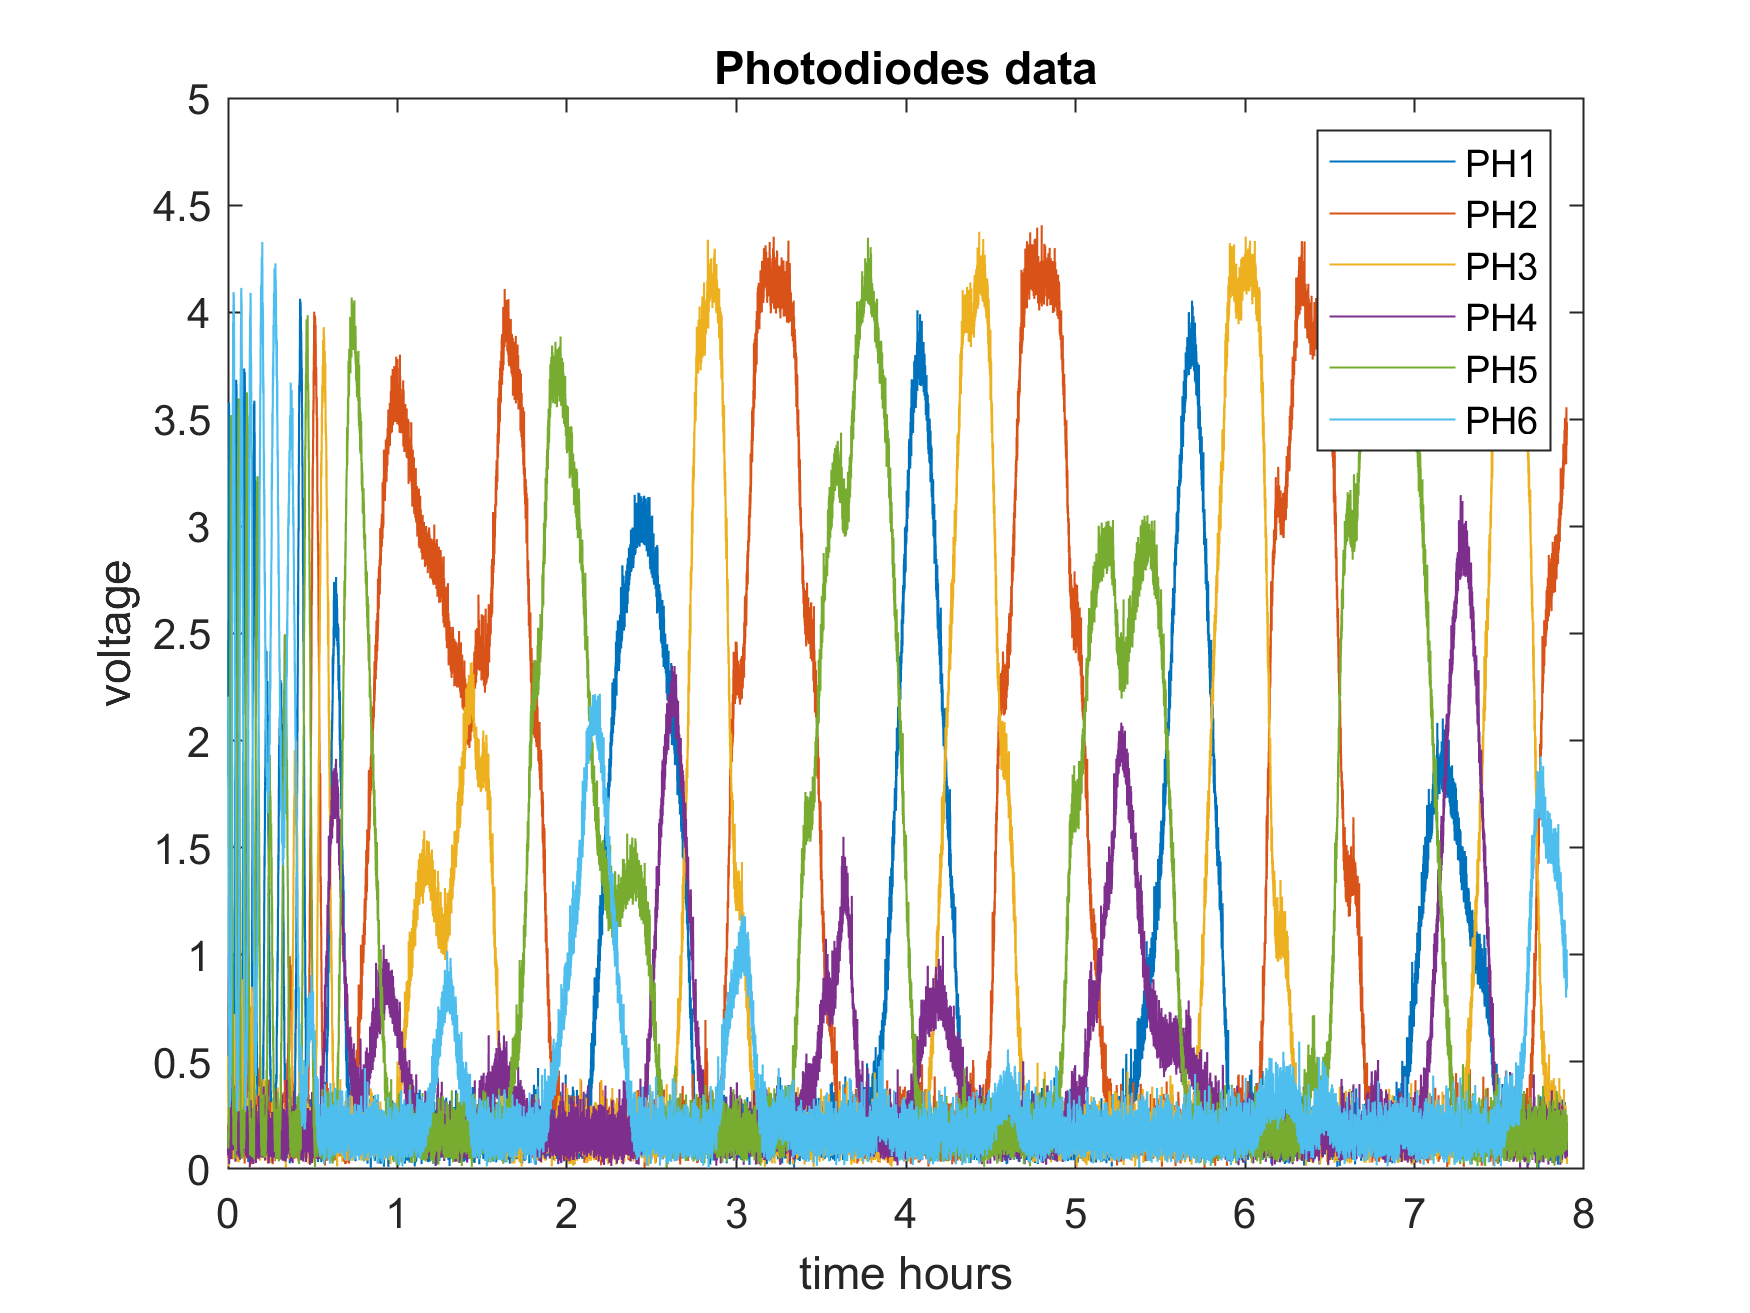
\includegraphics[width=0.7\linewidth]{res/img/Nadir_no_EKF/Photodiode data.png}
        \caption{Photodiode data}
        \label{fig:PhotodiodeData}
    \end{figure}

    \item \textbf{Sun Position Algorithm Performance }\\
    In the following section the performance of the developed Sun position algorithm estimator
    that uses the photodiodes and the temperature sensors is presented. The plots show two different lines, on the one hand
    an orange line which indicatess the real position of the sun, and on the other hand a blue line which
    indicates the estimation of the algorithm. It can be observed that the performance of the estimation is degradatedd
    by the noise of the photodiodes, the less noise the better estimation.
    \begin{figure}[H]
        \centering
        \begin{minipage}{0.32\linewidth}
            \centering
            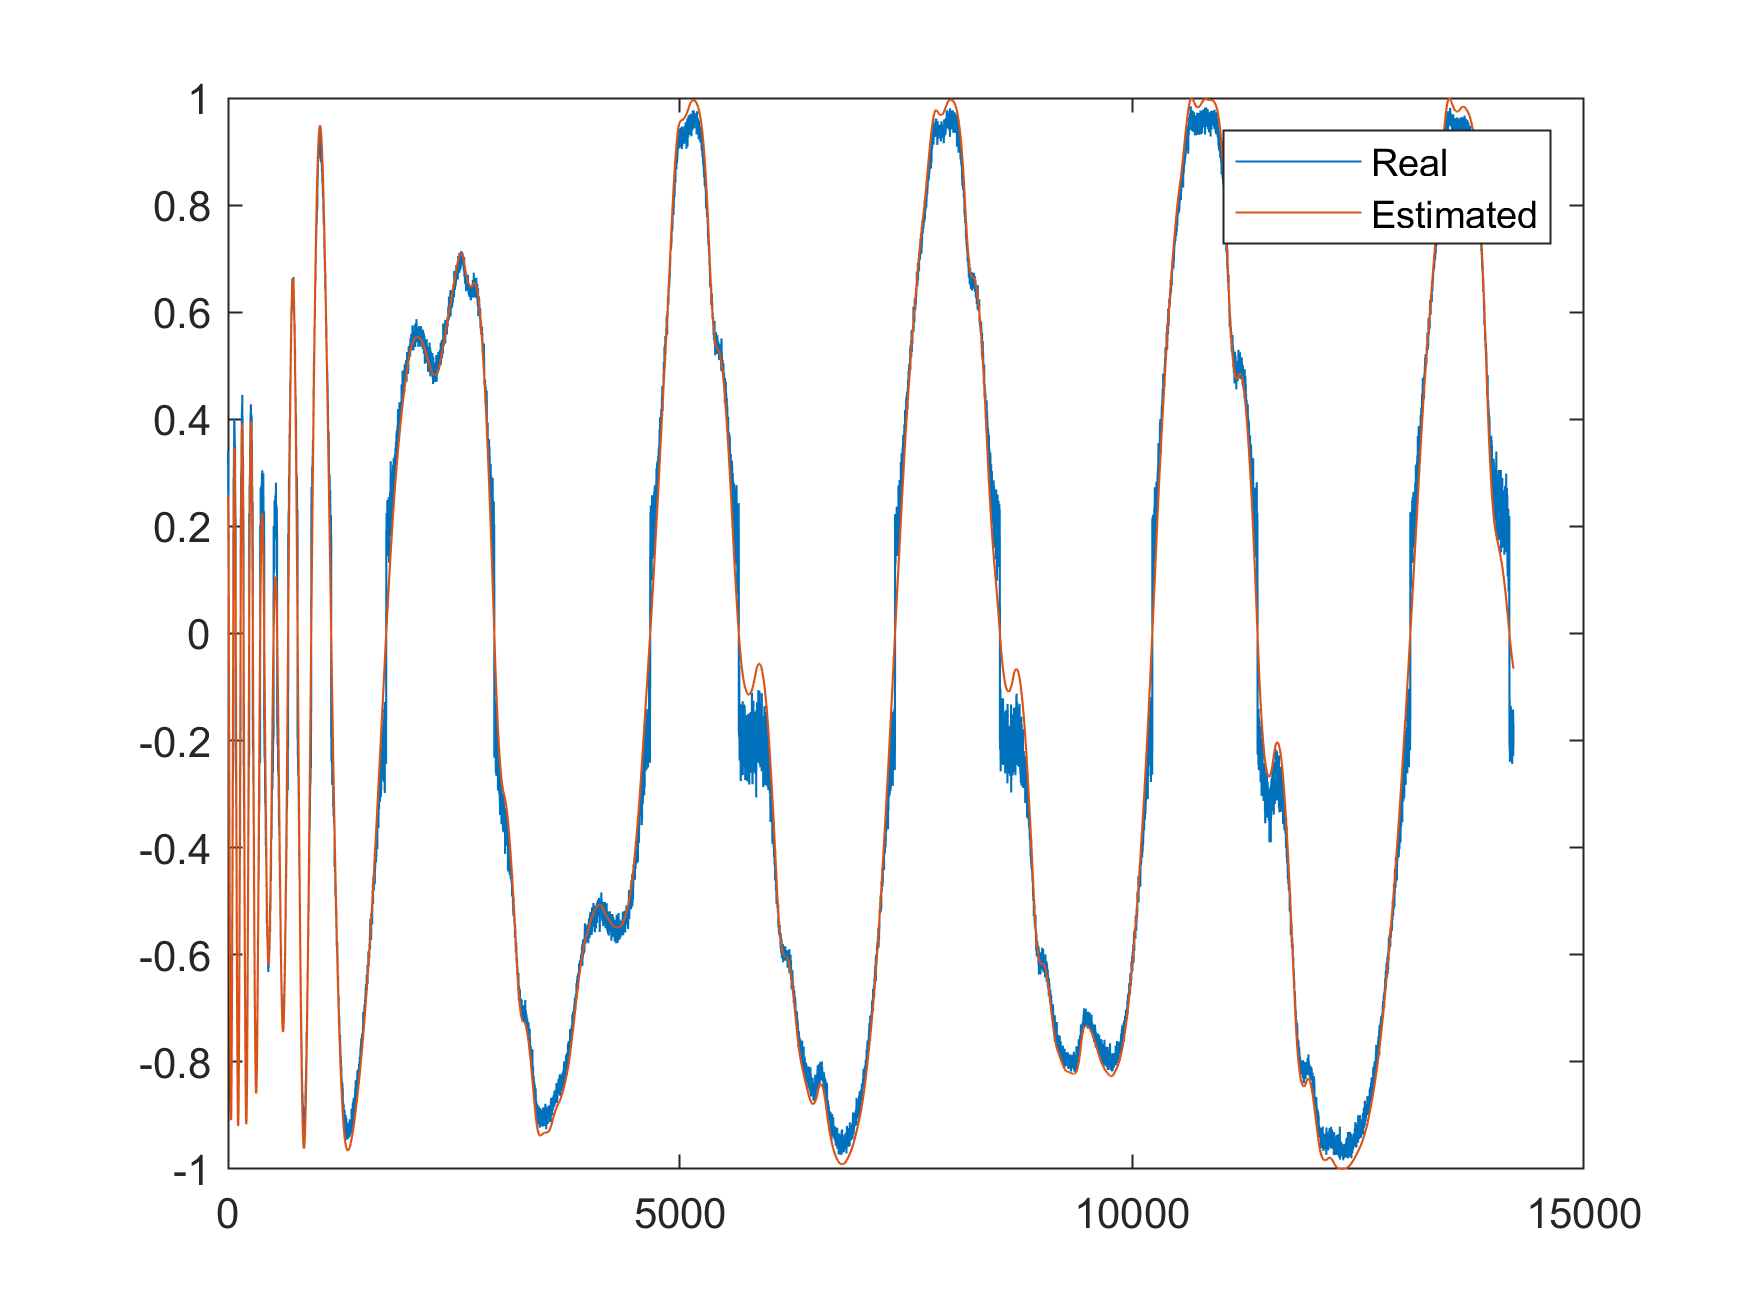
\includegraphics[width=0.95\linewidth]{res/img/Nadir_no_EKF/Sun position (ECI) X Axis.png}
            \caption{Sun position (ECI) X Axis}
            \label{fig:SunPositionECIX}
        \end{minipage}\hfill
        \begin{minipage}{0.32\linewidth}
            \centering
            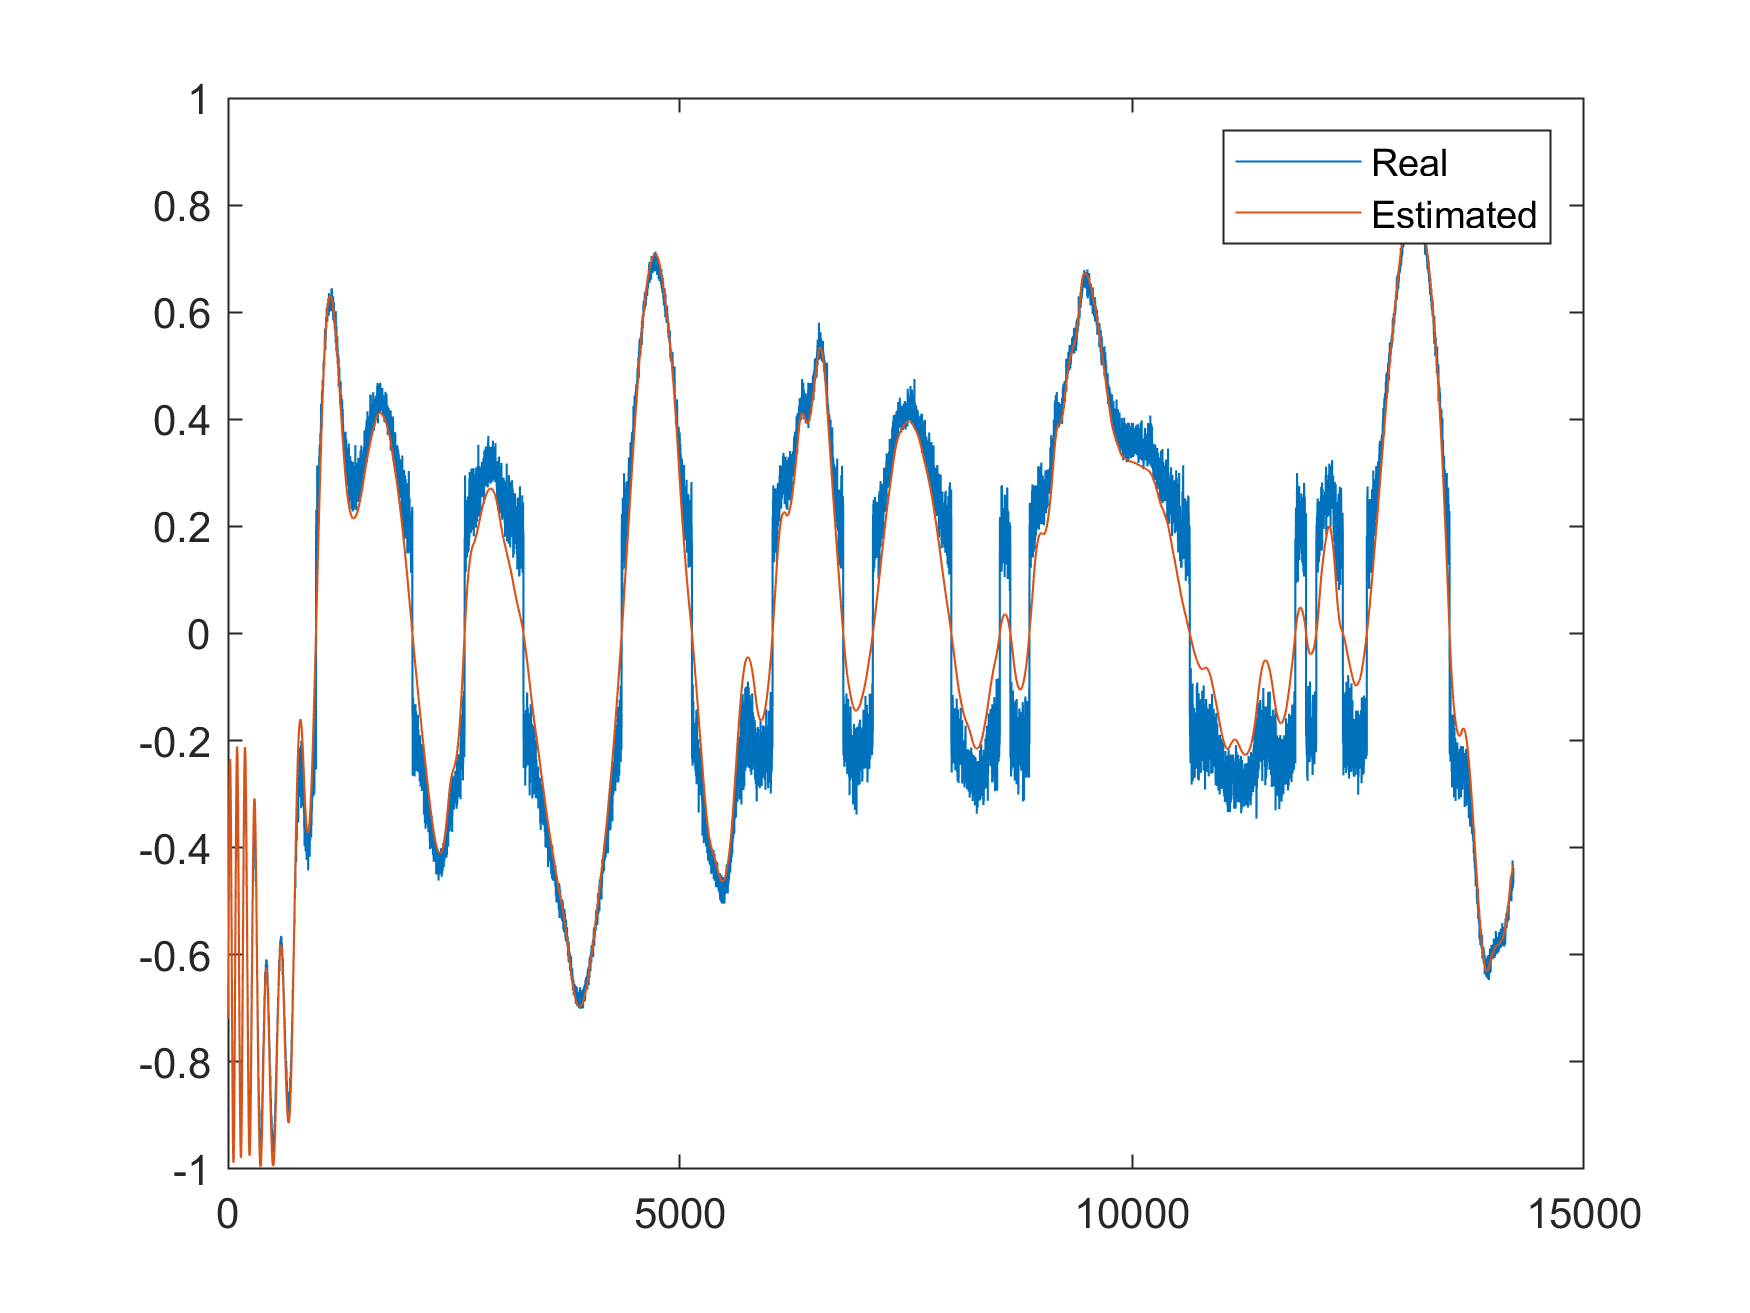
\includegraphics[width=0.95\linewidth]{res/img/Nadir_no_EKF/Sun position (ECI) Y Axis.png}
            \caption{Sun position (ECI) Y Axis}
            \label{fig:SunPositionECIY}
        \end{minipage}\hfill
        \begin{minipage}{0.32\linewidth}
            \centering
            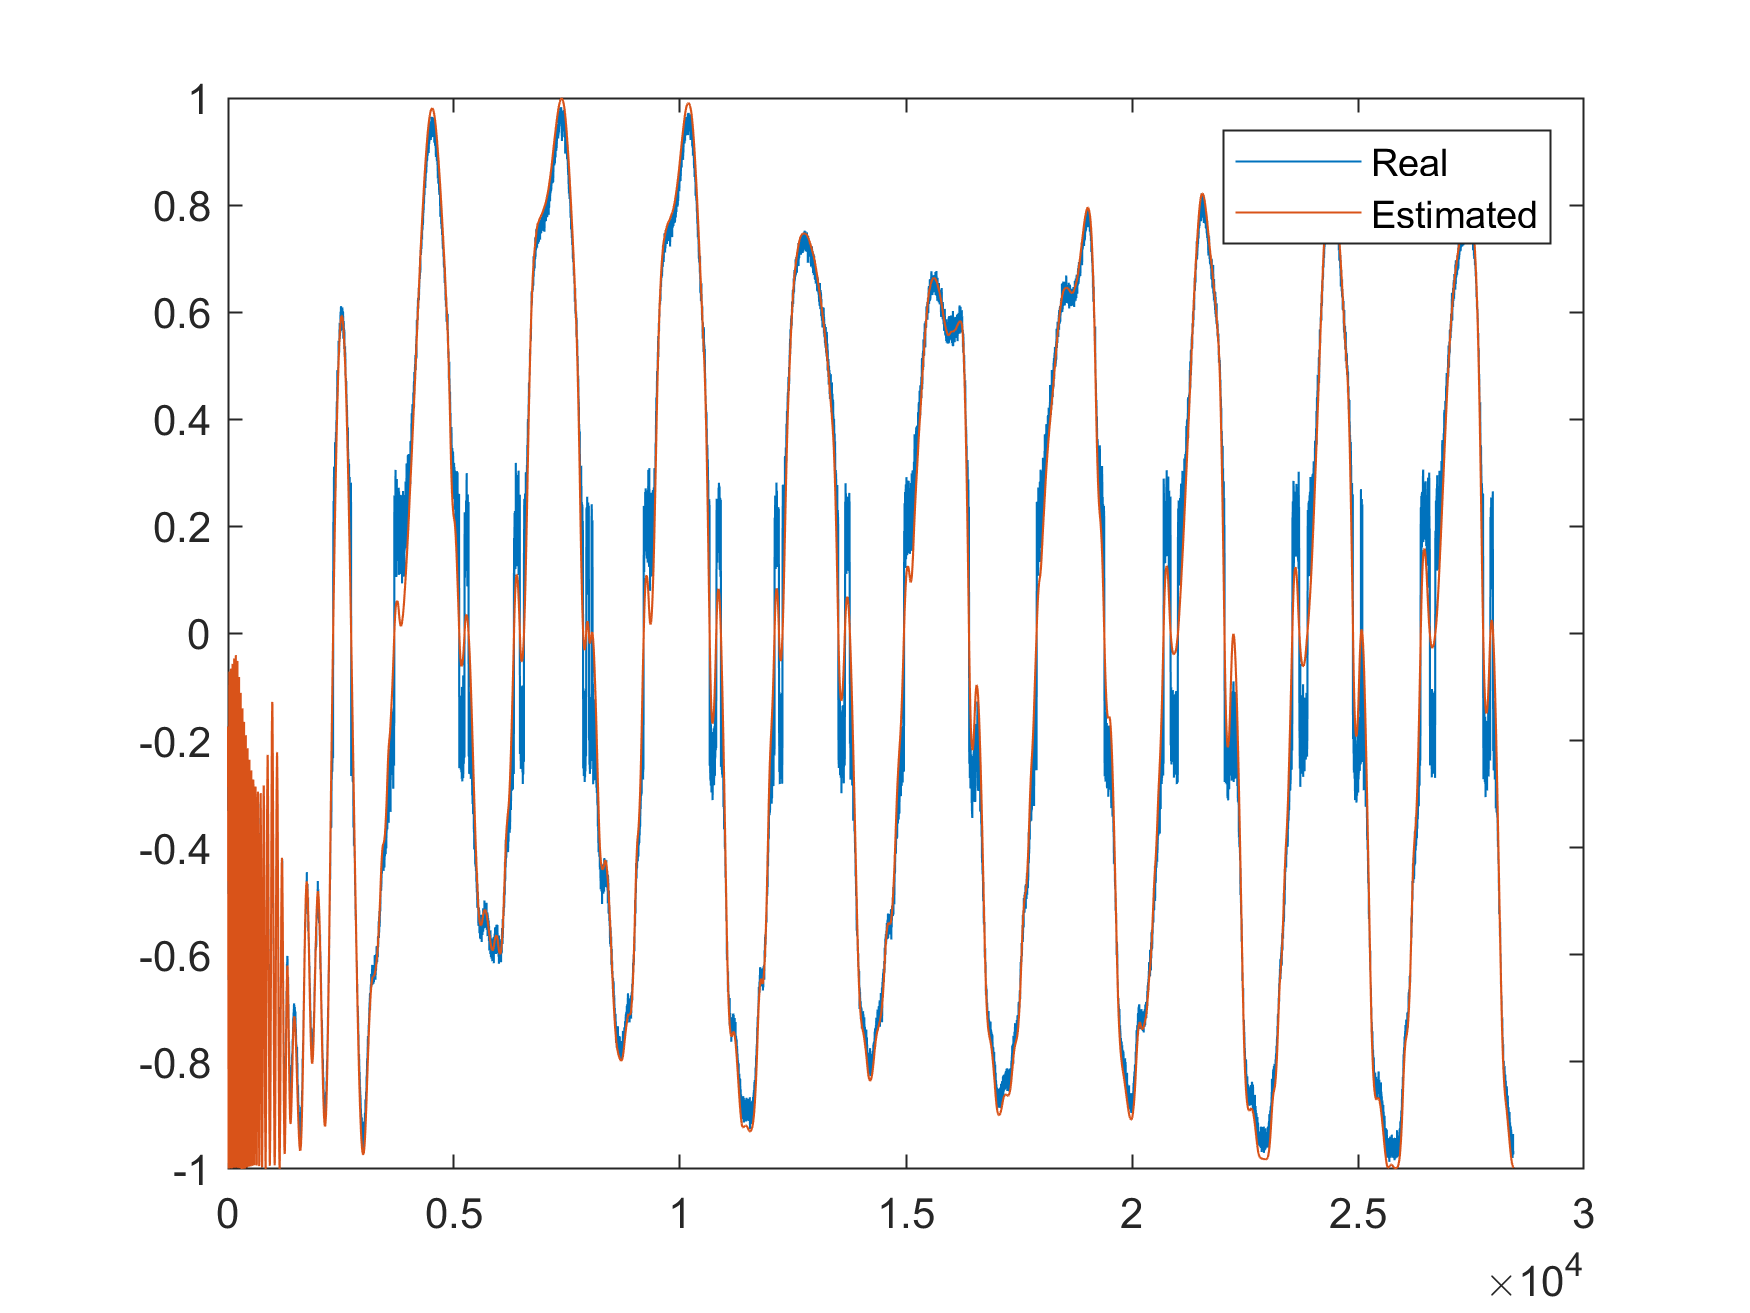
\includegraphics[width=0.95\linewidth]{res/img/Nadir_no_EKF/Sun position (ECI) Z Axis.png}
            \caption{Sun position (ECI) Z Axis}
            \label{fig:SunPositionECIZ}
        \end{minipage}
    \end{figure}

    \item \text{Magnetic Field Model}\\
    In this section the propagated magnetic field over the simulation is presented. The model as explained in 
    the previous sections is based on the tilted dipole model to reduce as much as possible the simulation time.
    \begin{figure}[H]
        \centering
        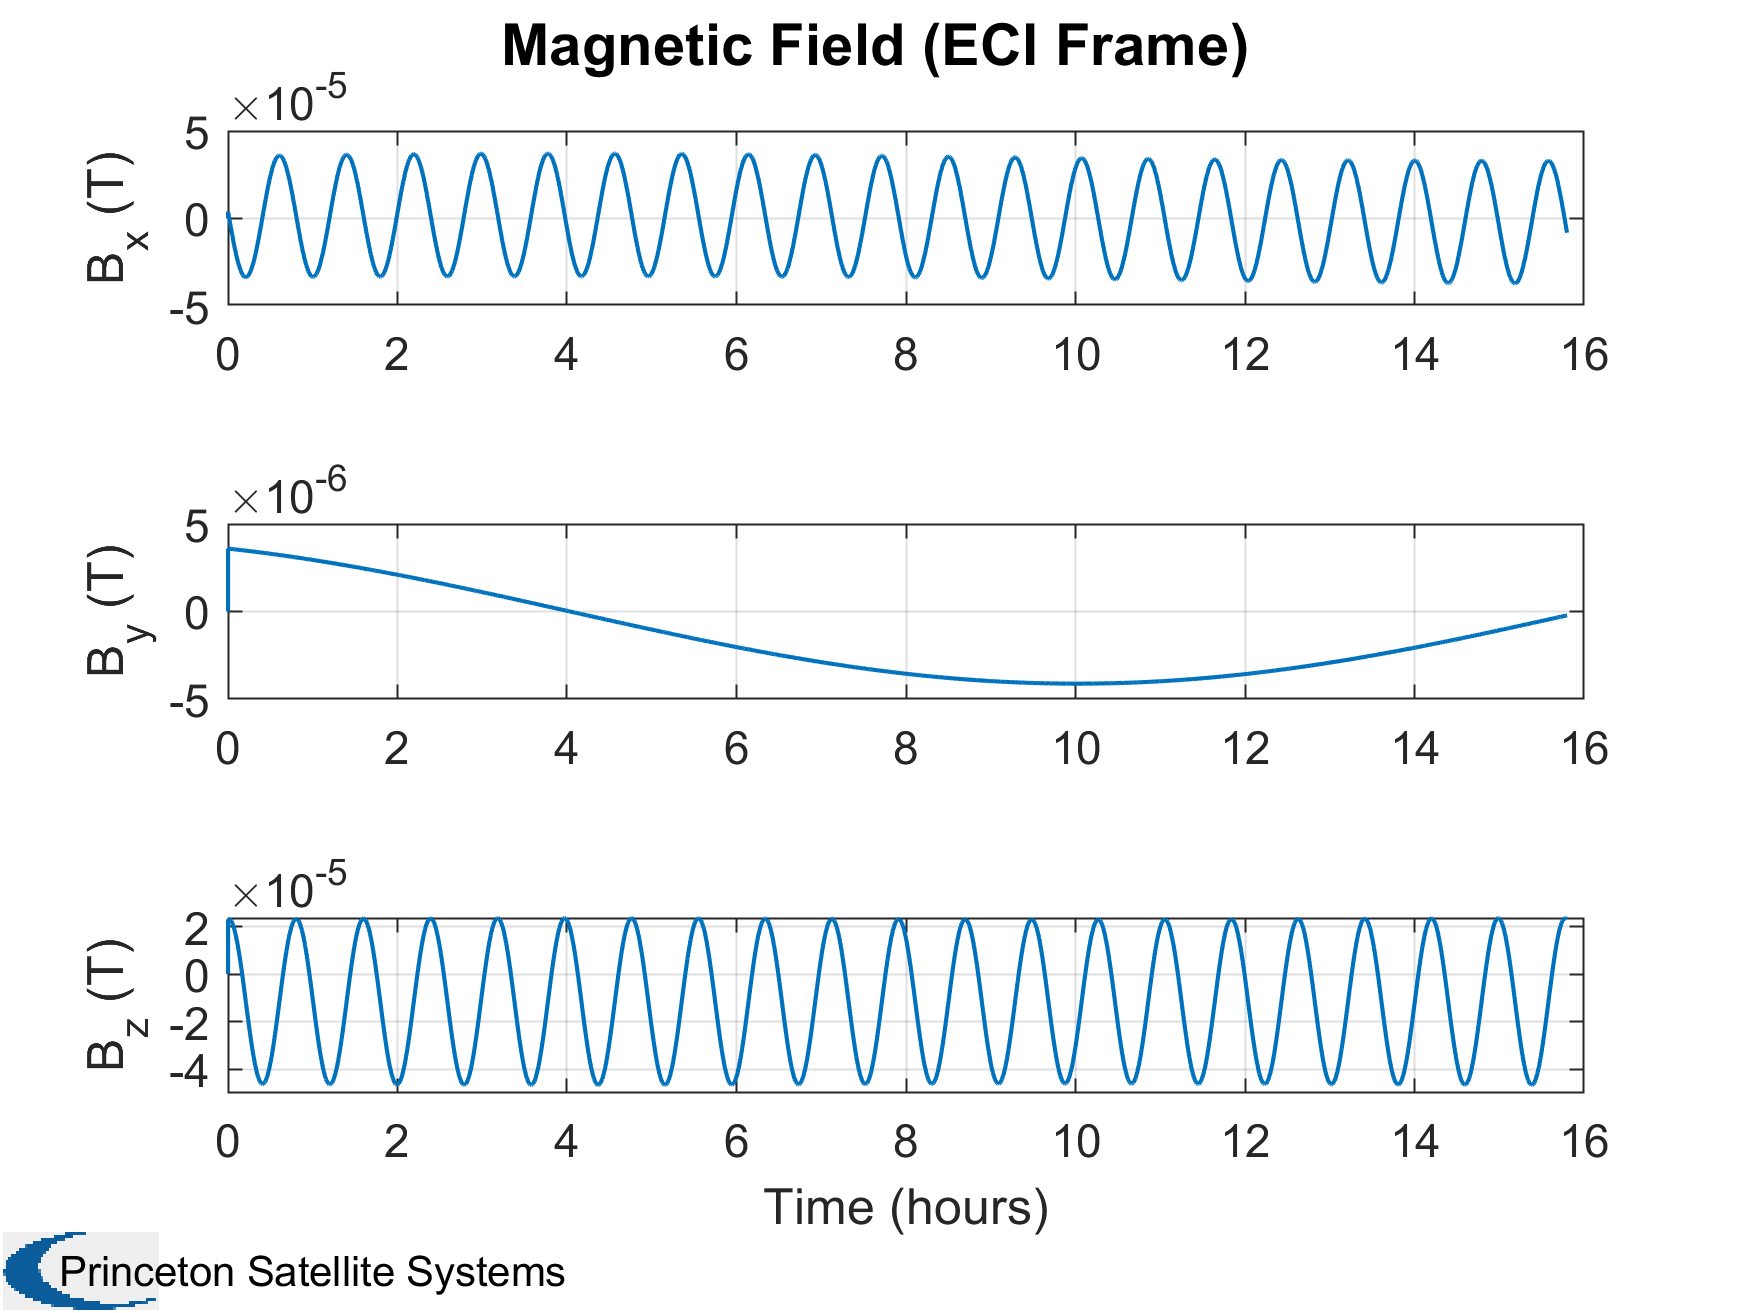
\includegraphics[width=0.7\linewidth]{res/img/Nadir_no_EKF/Magnetic Field (ECI Frame).png}
        \caption{Magnetic Field (ECI Frame)}
        \label{fig:MagneticFieldECI}
    \end{figure}

    \item \textbf{Real angular Velocity}\\
    In the following plot it is shown the angular velocity propagated in each iteration of the simulation. In short
    words it is the real angular velocity in which the satellite is rotating due to the torques affecting the PQ.
    
    \begin{figure}[H]
        \centering
        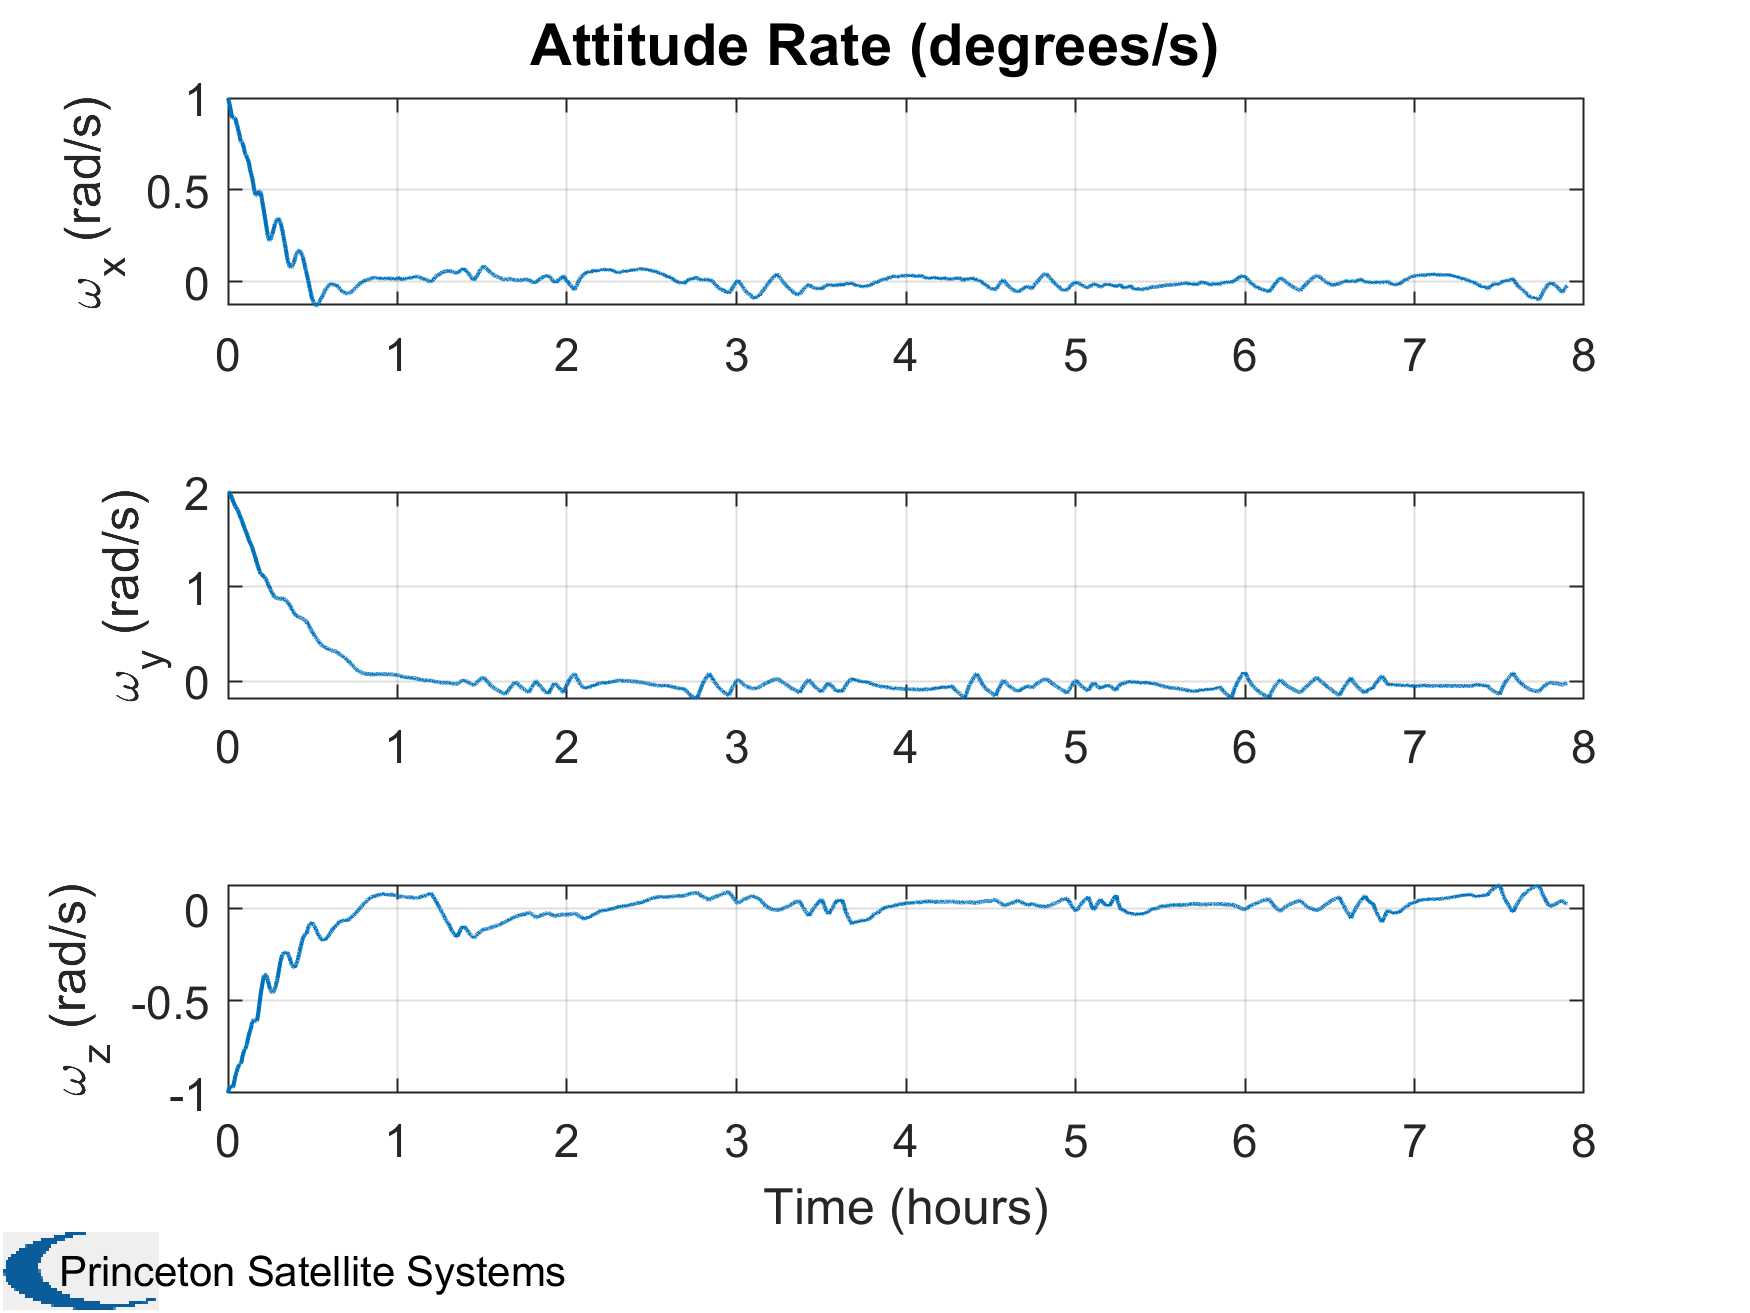
\includegraphics[width=0.7\linewidth]{res/img/Nadir_no_EKF/Attitude Rate.png}
        \caption{Attitude Rate}
        \label{fig:AttitudeRate}
    \end{figure}

    \item \textbf{Generated torque}\\
    In the pictures below it is observed the generated torque by the magnetic moment generated by the magnetorquers.
    This torque is the required torque to be applied in order to conduct the Nadir Pointing mode.
    \begin{figure}[H]
        \centering
        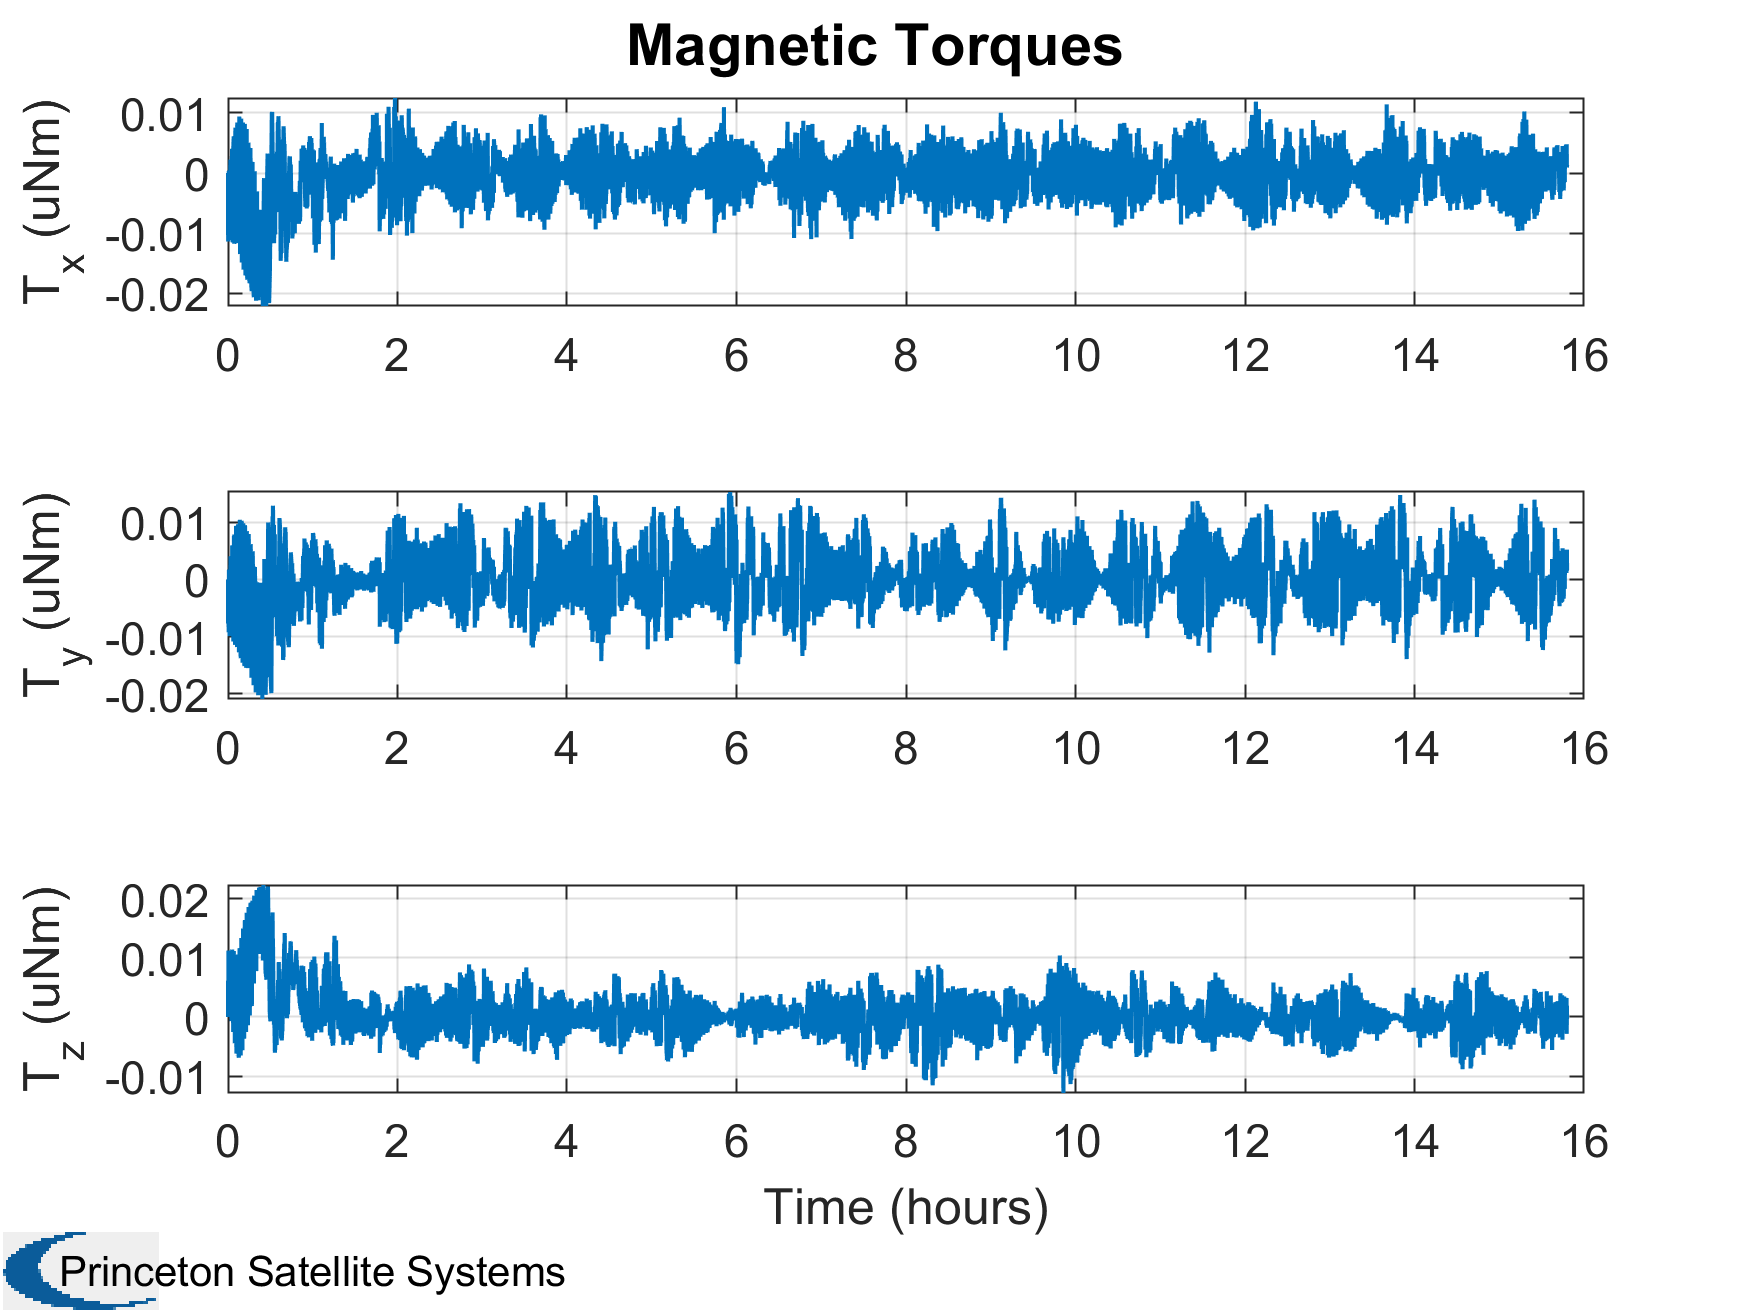
\includegraphics[width=0.7\linewidth]{res/img/Nadir_no_EKF/Magnetic Torques.png}
        \caption{Magnetic torque}
        \label{fig:Magnetic torque}
    \end{figure}

    \item \textbf{Injected Intesity}\\
    The following plots show the required intensity to be injected in the magnetorquers in order to generate the
    necessary magnetic moment to conduct the Nadir Pointing mode. It can be observed that the intensity is quatified due 
    to the limitations of the magnetorquer driver, as it can only inject from 0.5 mA to 32 mA in steps of 0.5 mA. If the
    computed intensity exceeds the maximum value, the simulation limits this intensity to 32 mA, as can be seen in the first
    hour of the simulation. 
    \begin{figure}[H]
        \centering
        \begin{minipage}{0.32\linewidth}
            \centering
            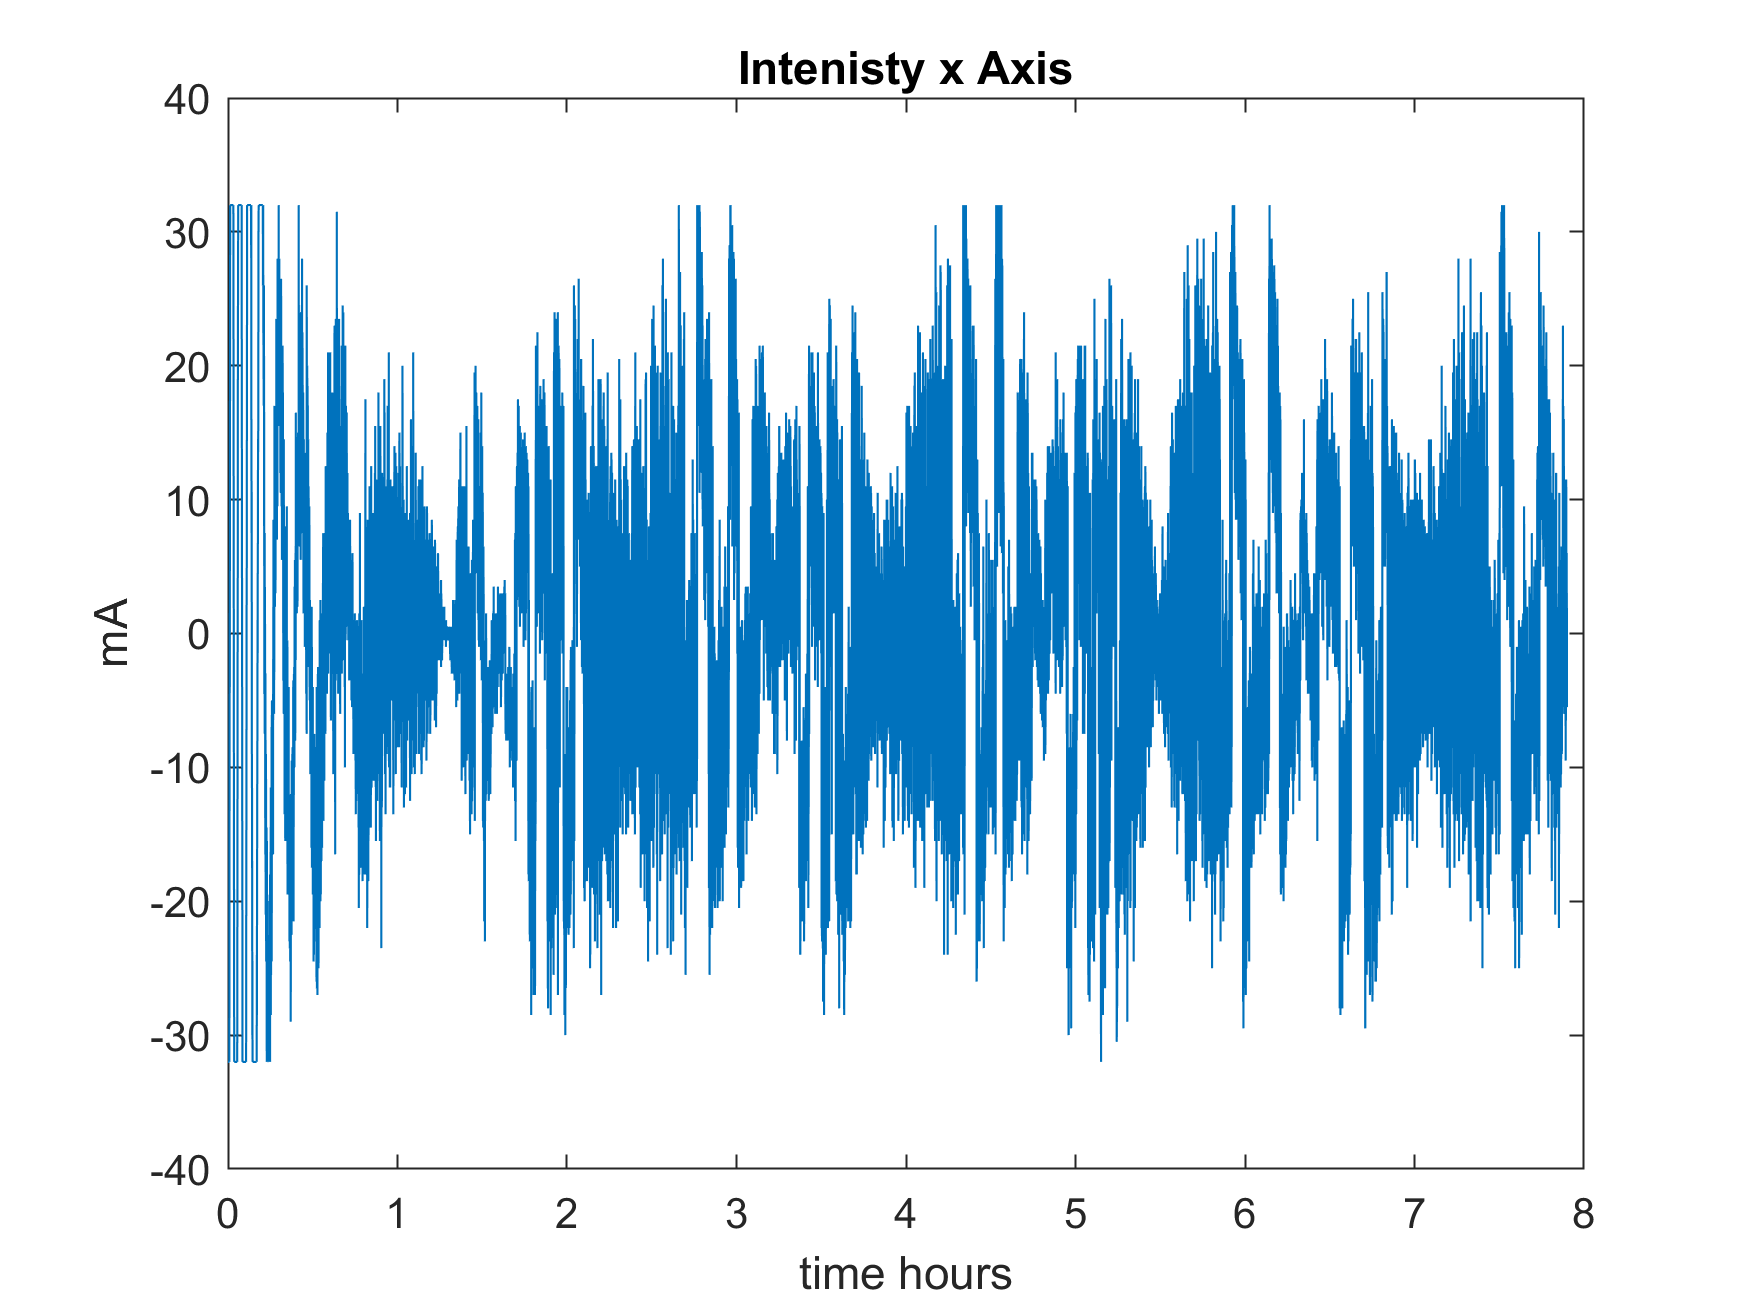
\includegraphics[width=0.95\linewidth]{res/img/Nadir_no_EKF/Intenisty x Axis.png}
            \caption{Intensity x Axis}
            \label{fig:IntensityX}
        \end{minipage}\hfill
        \begin{minipage}{0.32\linewidth}
            \centering
            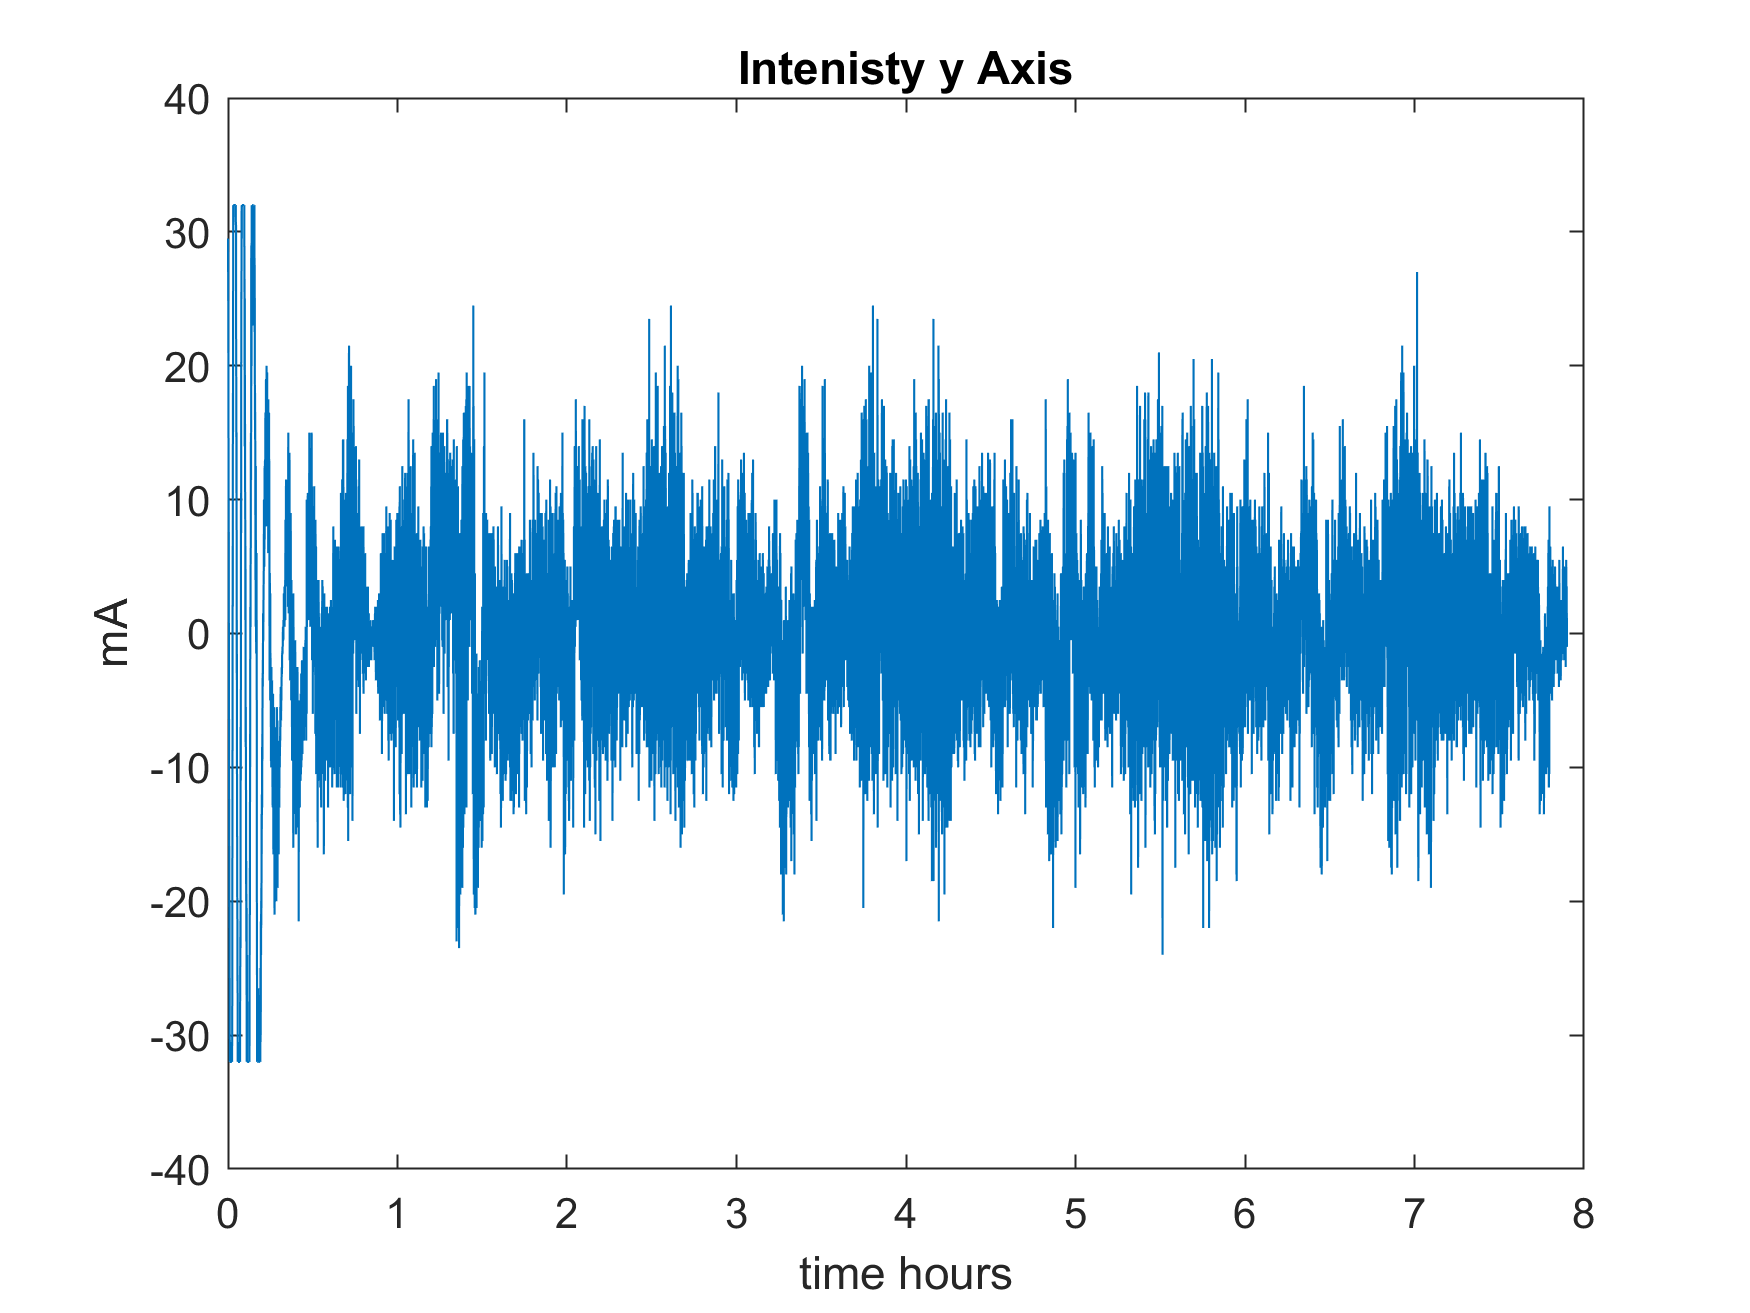
\includegraphics[width=0.95\linewidth]{res/img/Nadir_no_EKF/Intenisty y Axis.png}
            \caption{Intensity y Axis}
            \label{fig:IntensityY}
        \end{minipage}\hfill
        \begin{minipage}{0.32\linewidth}
            \centering
            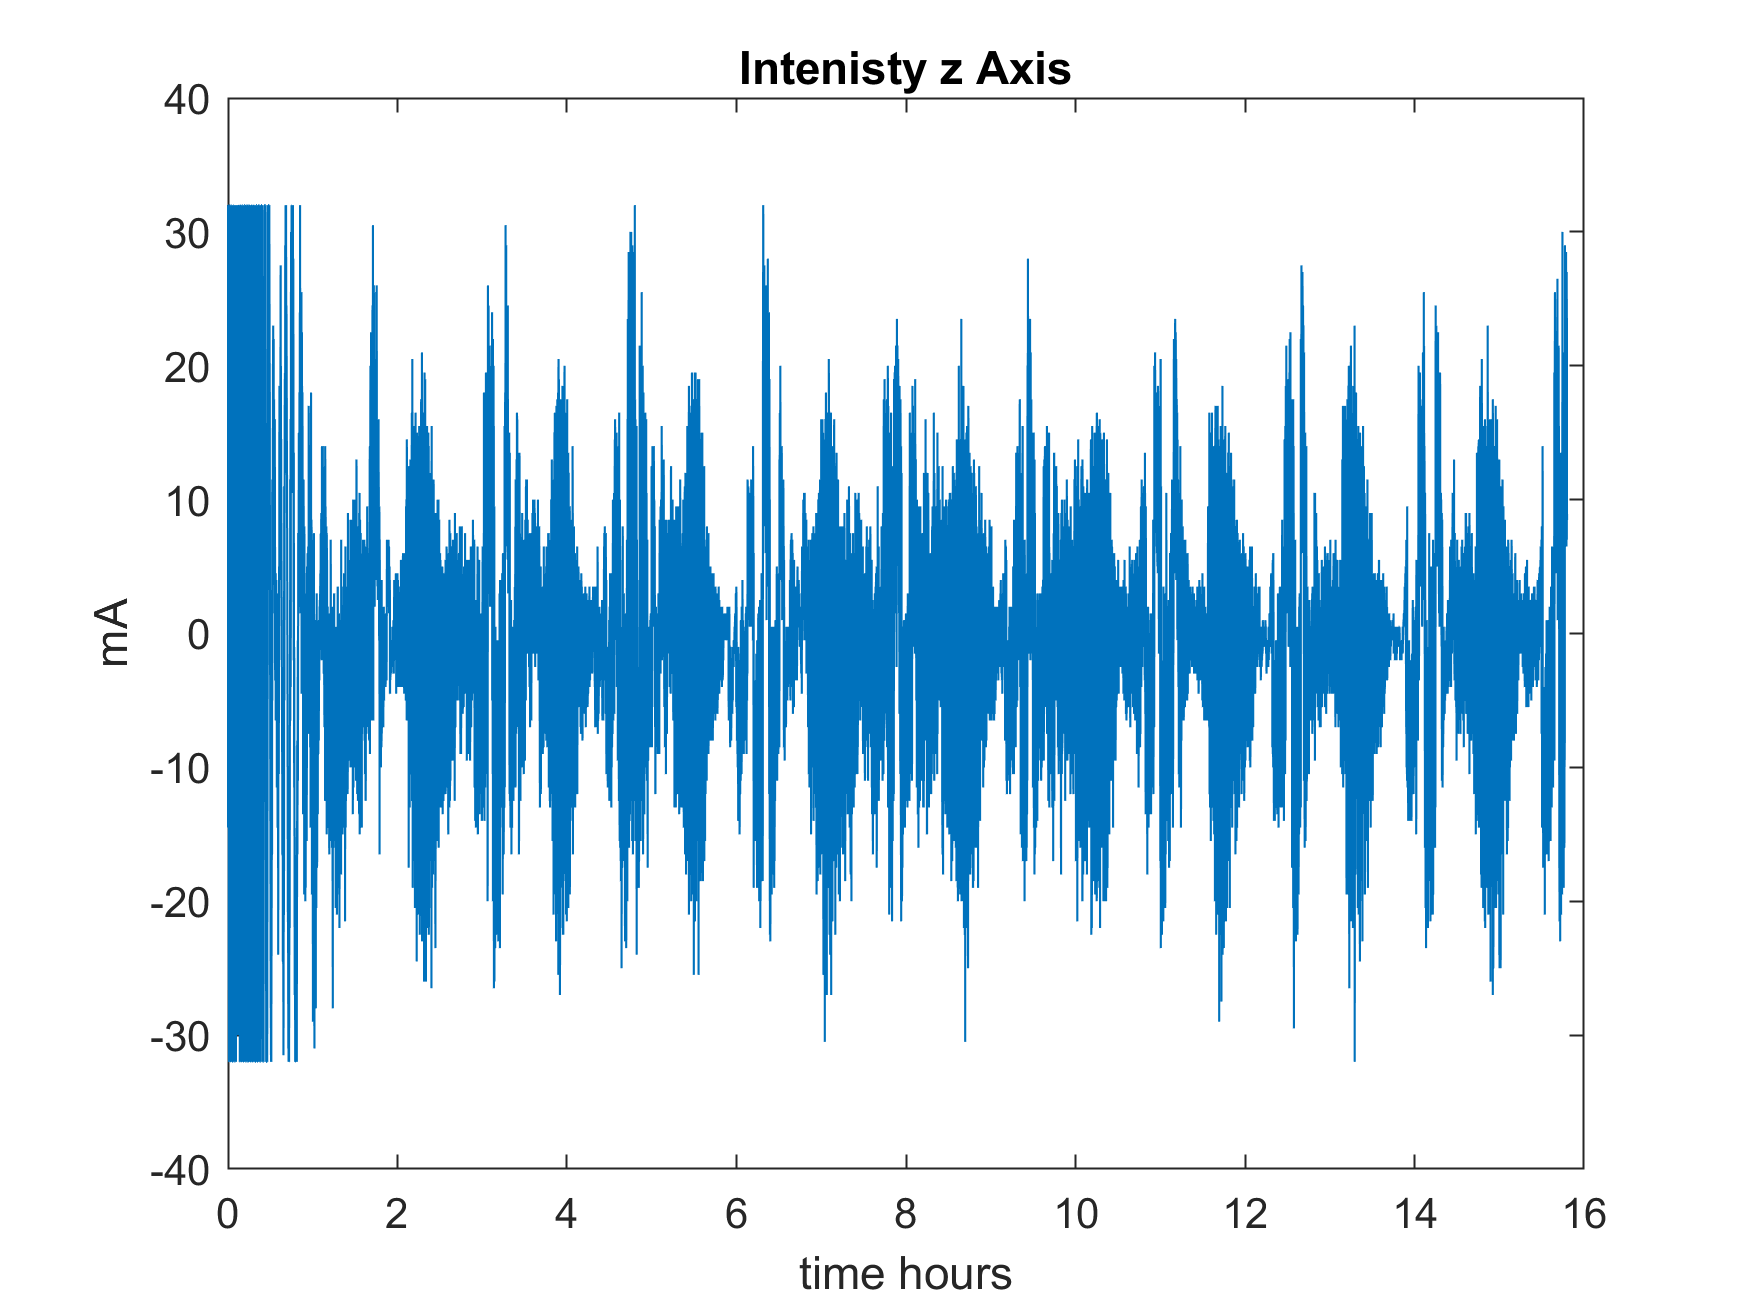
\includegraphics[width=0.95\linewidth]{res/img/Nadir_no_EKF/Intenisty z Axis.png}
            \caption{Intensity z Axis}
            \label{fig:IntensityZ}
        \end{minipage}
    \end{figure}

    \item \textbf{Attitude quaternion}\\
    The following plot indicates the attitude quaternion of the PQ. The selected quaternion is the
    one representing the rotation from the LVLH frame to the body frame.
    This quaternion is selected to show the performance of the Nadir Pointing mode, as the quaternion indicating that
    the PQ is pointing to the Nadir angle has a very simple representation, which is the quaternion [+-1, 0, 0, 0]. In the 
    plot can be observed that the scalar component (qs) of the quaternion of the PQ is de desired one. Nevertheless,
    the vectorial part is where can be observed the effect of the noise of the sensors and the errors in the 
    estimations, they do not converge exactly to zero; instead, residual errors remain, resulting in some inaccuracy in the pointing.


    \begin{figure}[H]
        \centering
        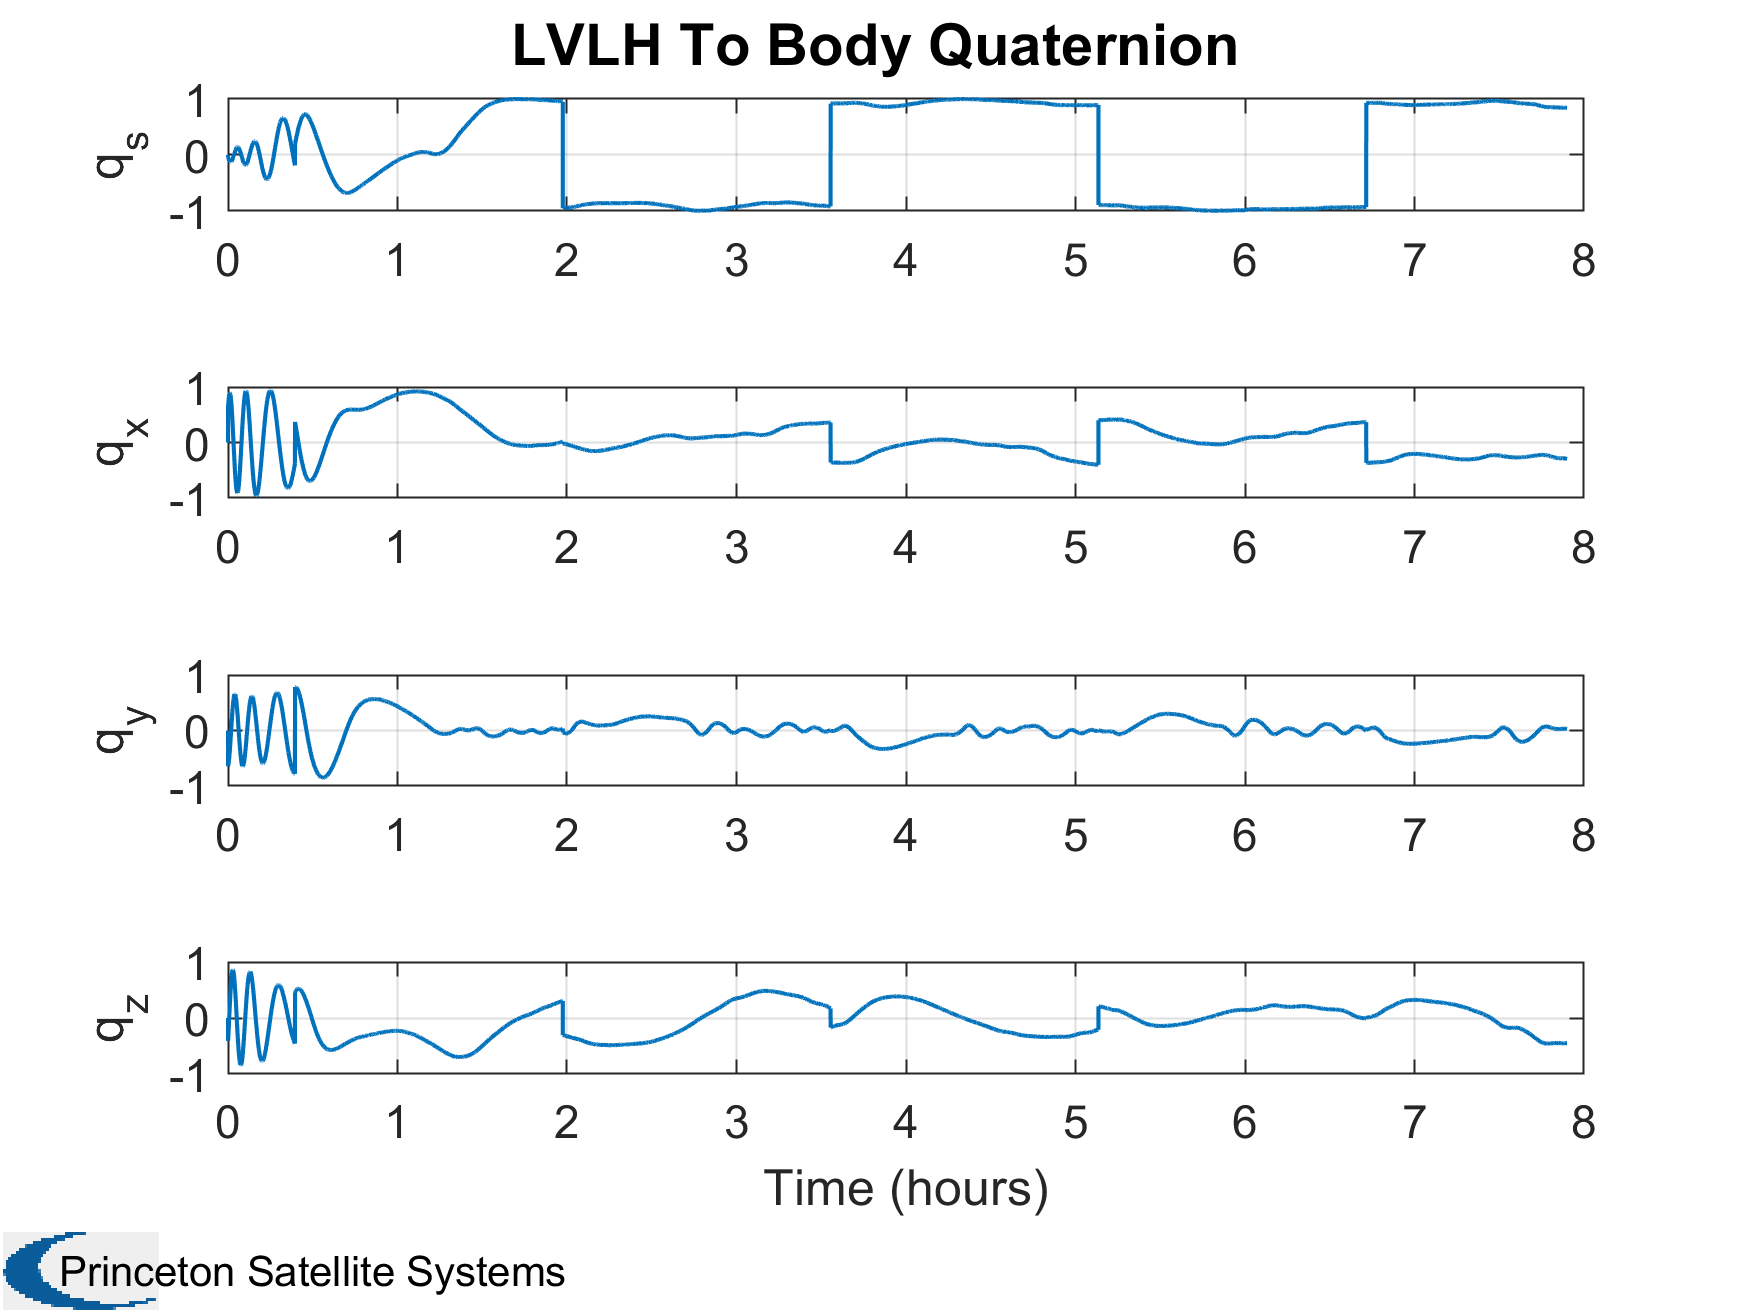
\includegraphics[width=0.7\linewidth]{res/img/Nadir_no_EKF/LVLH To Body Quaternion.png}
        \caption{LVLH To Body Quaternion}
        \label{fig:LVLHToBodyQuaternion}
    \end{figure}

\end{itemize}

\noindent In the picture below can be observed the angle between the nadir vector and the +Z unitary vector of the body frame. 
Additionally, there is a line marking the 20º limit, which is the requirement of the Nadir Pointing mode. 
Overall, the results show that the requirement is not met, therefore, a solution to improve the performance has to be implemented.
The proposed solution is the implementation of an Extended Kalman Filter (EKF) to improve the attitude estimation, which will be presented in the next section.

\begin{figure}[H]
    \centering
    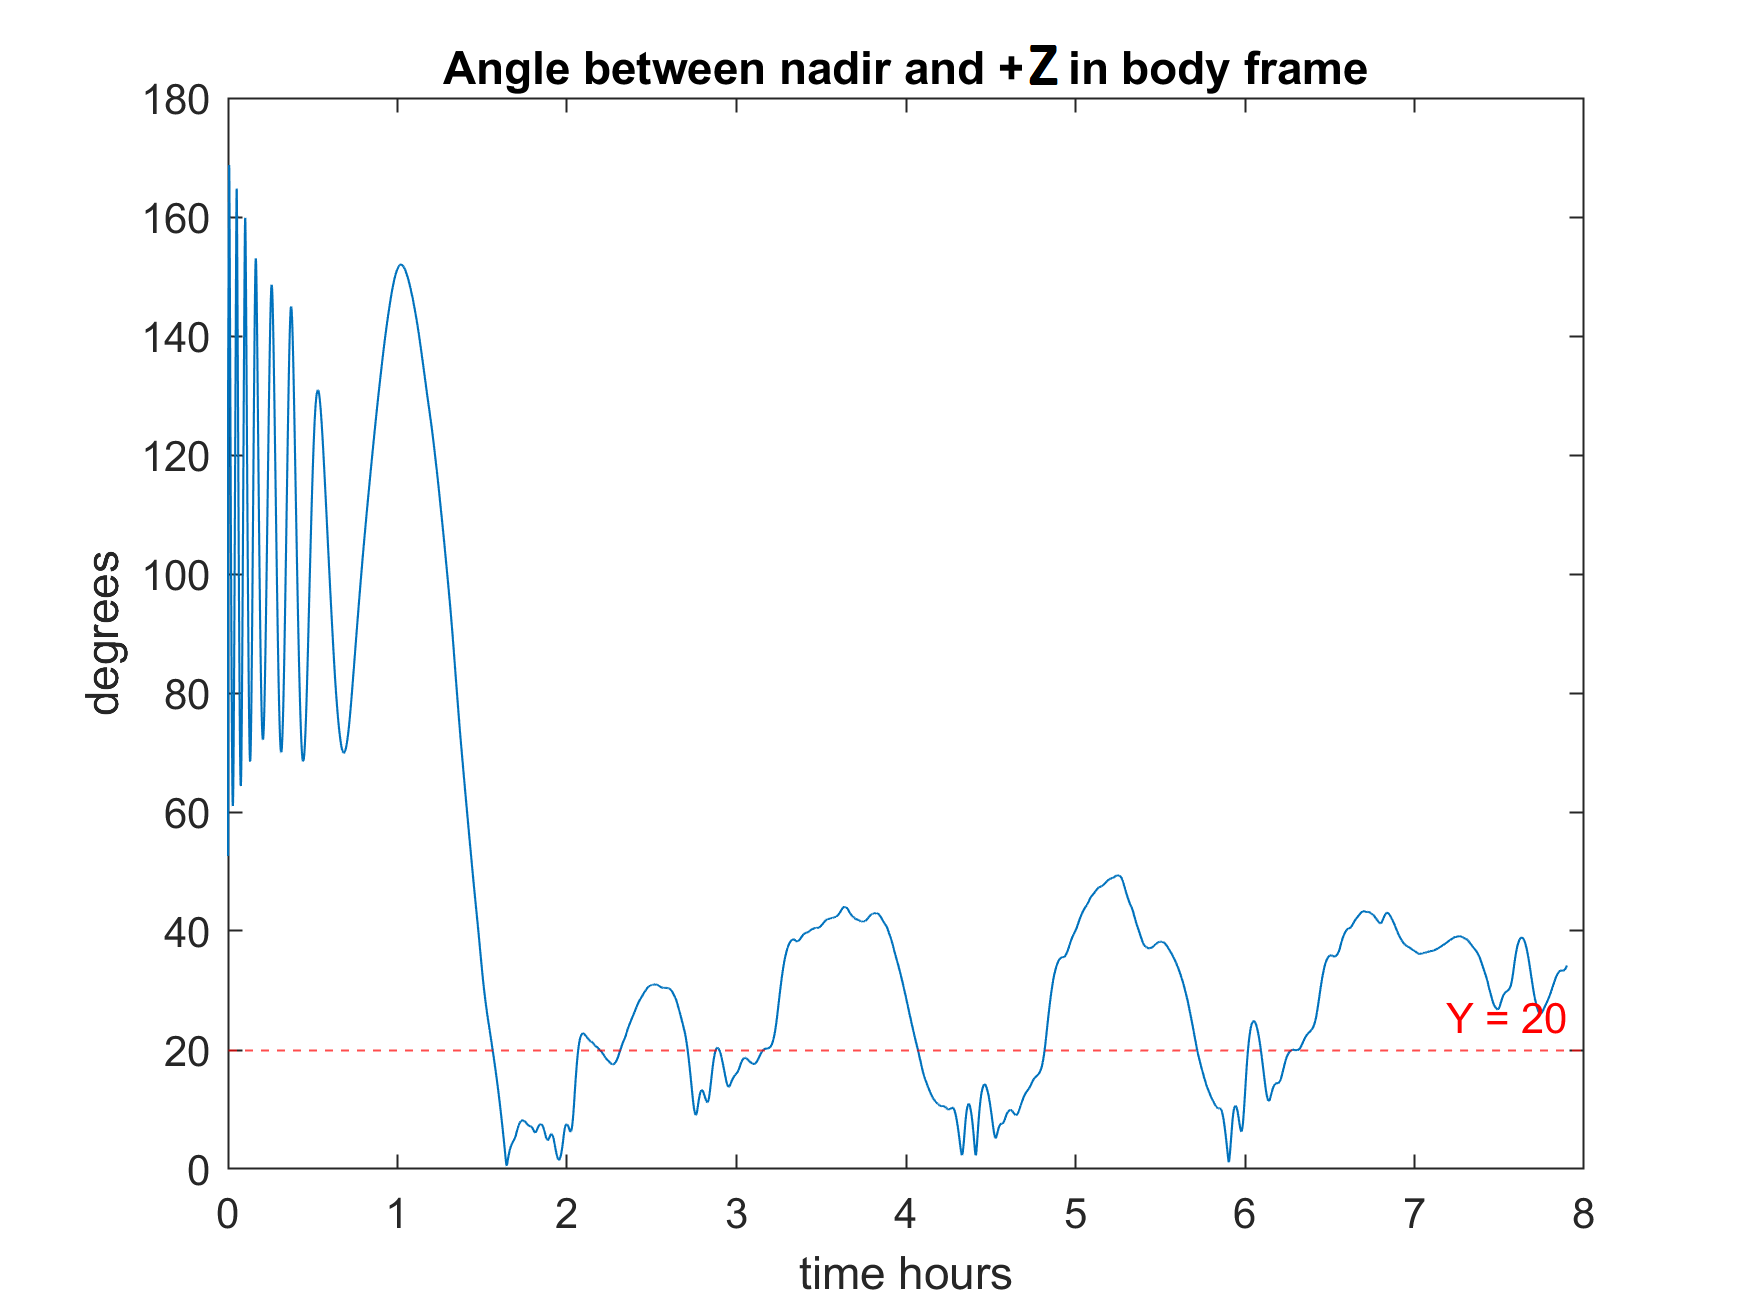
\includegraphics[width=0.7\linewidth]{res/img/Nadir_no_EKF/Angle between nadir and +Y.png}
    \caption{Angle between nadir and +Y}
    \label{fig:AngleNadirY}
\end{figure}

\subsubsection{Nadir pointing using an Extended Kalman Filter (EKF) for attitude determination}
In consequence of the results obtained in the previous seconds, the proposed solution to achieve
the requirement of the Payload is to implement an EKF to improve the attitude estimation. 
The EKF used is the one proposed in \cite{EKF}. This proposed EKF uses the manifold theory to update
the attitude quaternion, the covarianve matrix of the state and the angular velocity. Additionally, it uses measurements
from the gyroscope and the magnetometer to update the state of the EKF.\\

\noindent In this section the results of the simulation of the Nadir Pointing using the EKF are presented.
In addition, the performance of the EKF is analysed and compared with the performance of the Nadir Pointing mode without the EKF.

\begin{itemize}
    \item \textbf{External perturbations}\\
    In this section all the external perturbations affecting the PQ are presented.
    \begin{figure}[H]
        \centering
        \begin{minipage}{0.48\linewidth}
            \centering
            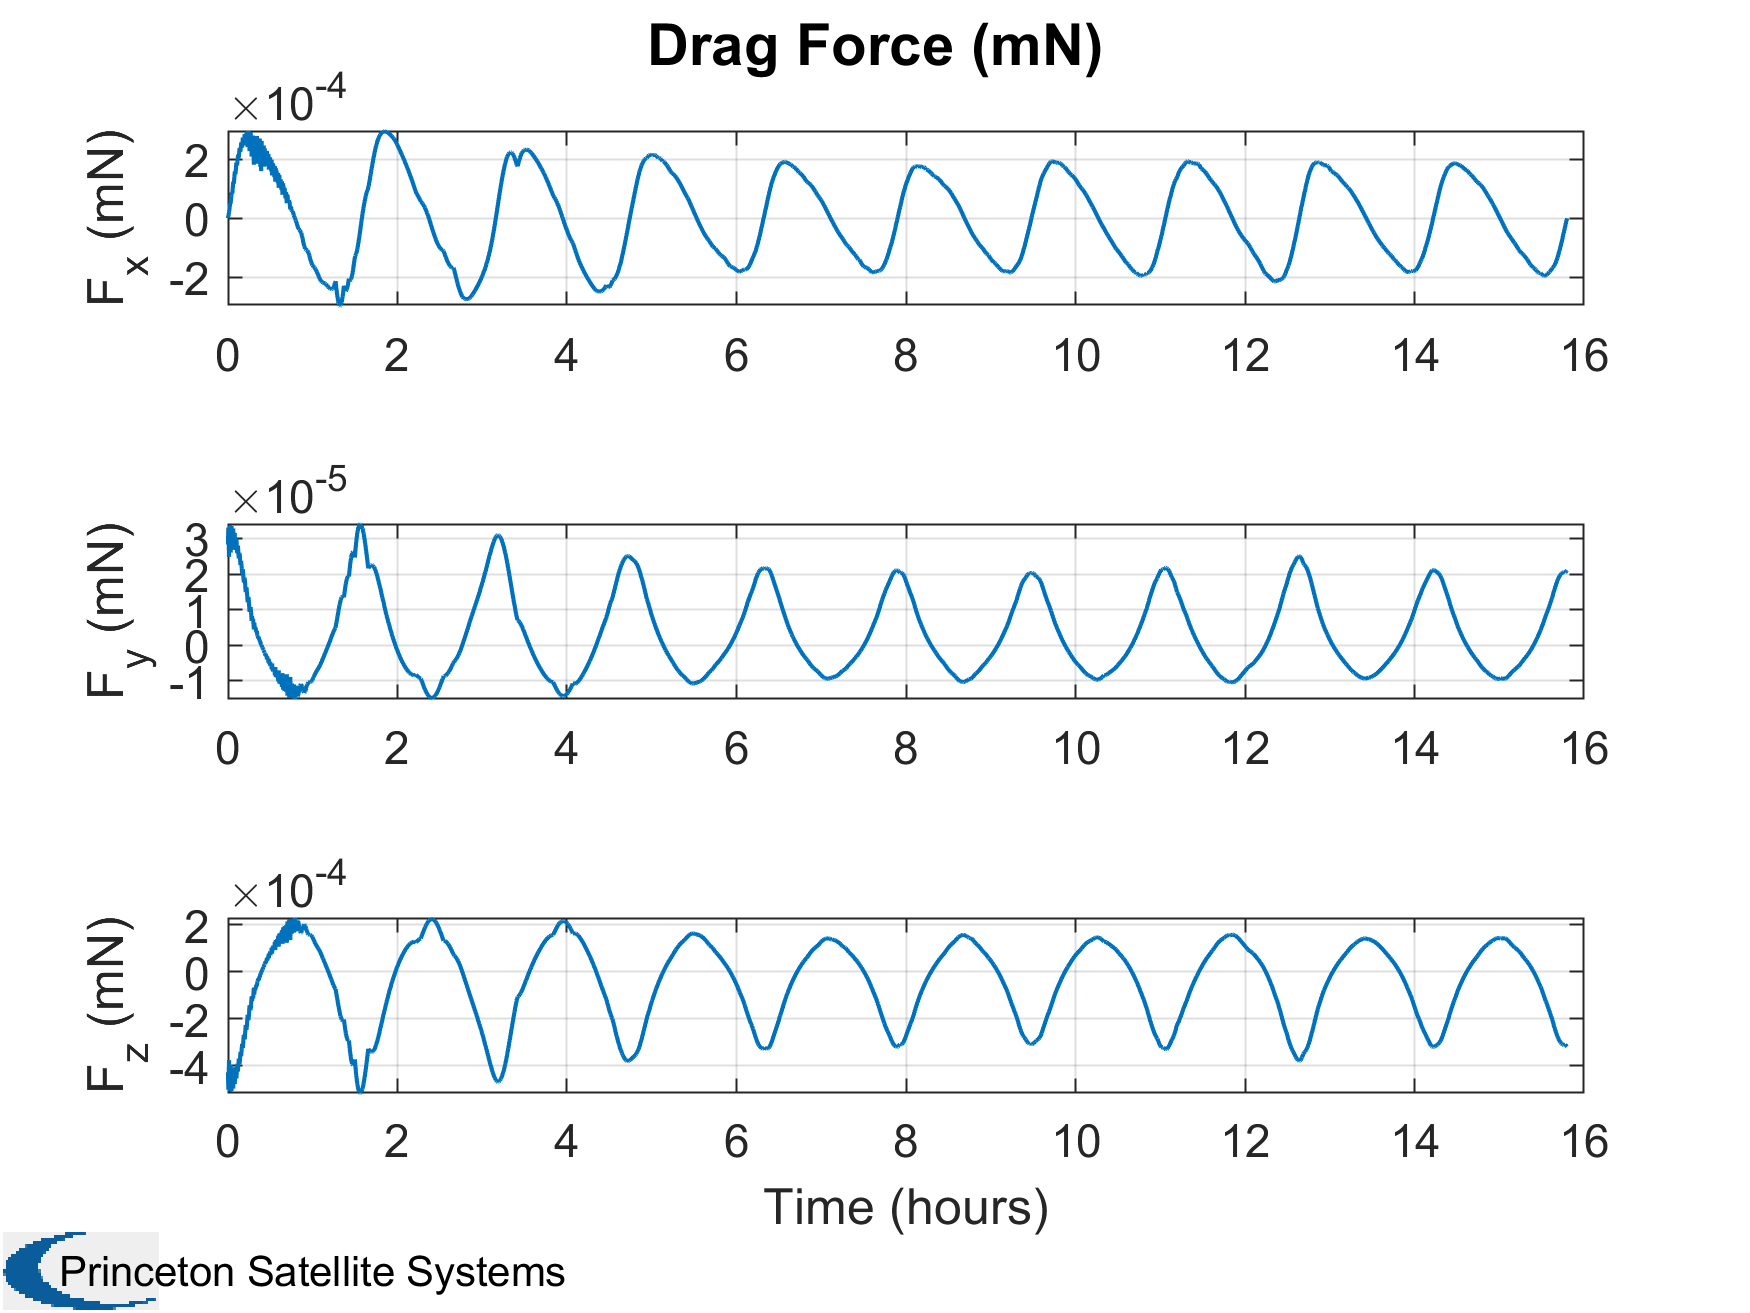
\includegraphics[width=0.95\linewidth]{res/img/Nadir_EKF/Simulations/Drag Force (mN).png}
            \caption{Drag Force (mN)}
        \end{minipage}\hfill
        \begin{minipage}{0.48\linewidth}
            \centering
            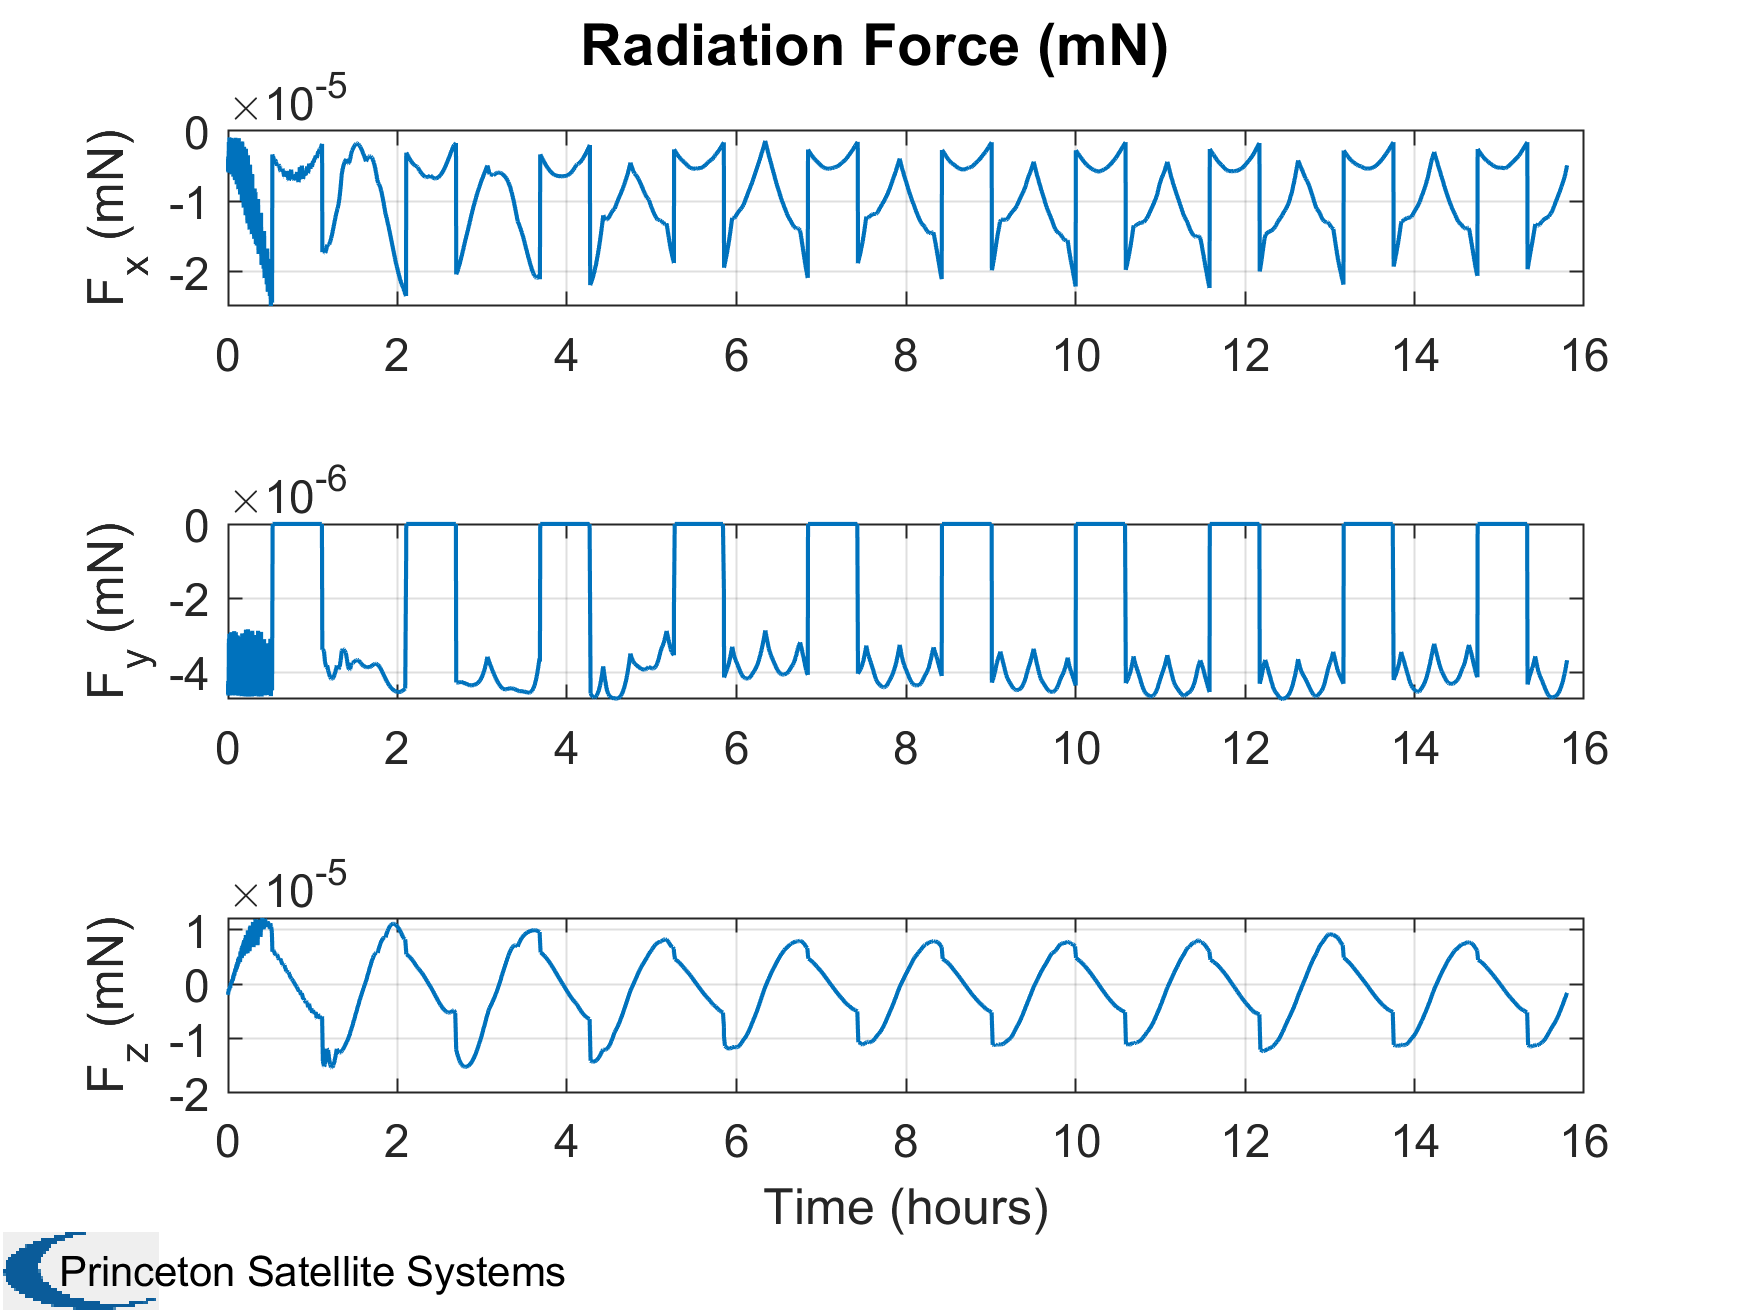
\includegraphics[width=0.95\linewidth]{res/img/Nadir_EKF/Simulations/Radiation Force (mN).png}
            \caption{Radiation Force (mN)}
        \end{minipage}
    \end{figure}

    \begin{figure}[H]
        \centering
        \begin{minipage}{0.48\linewidth}
            \centering
            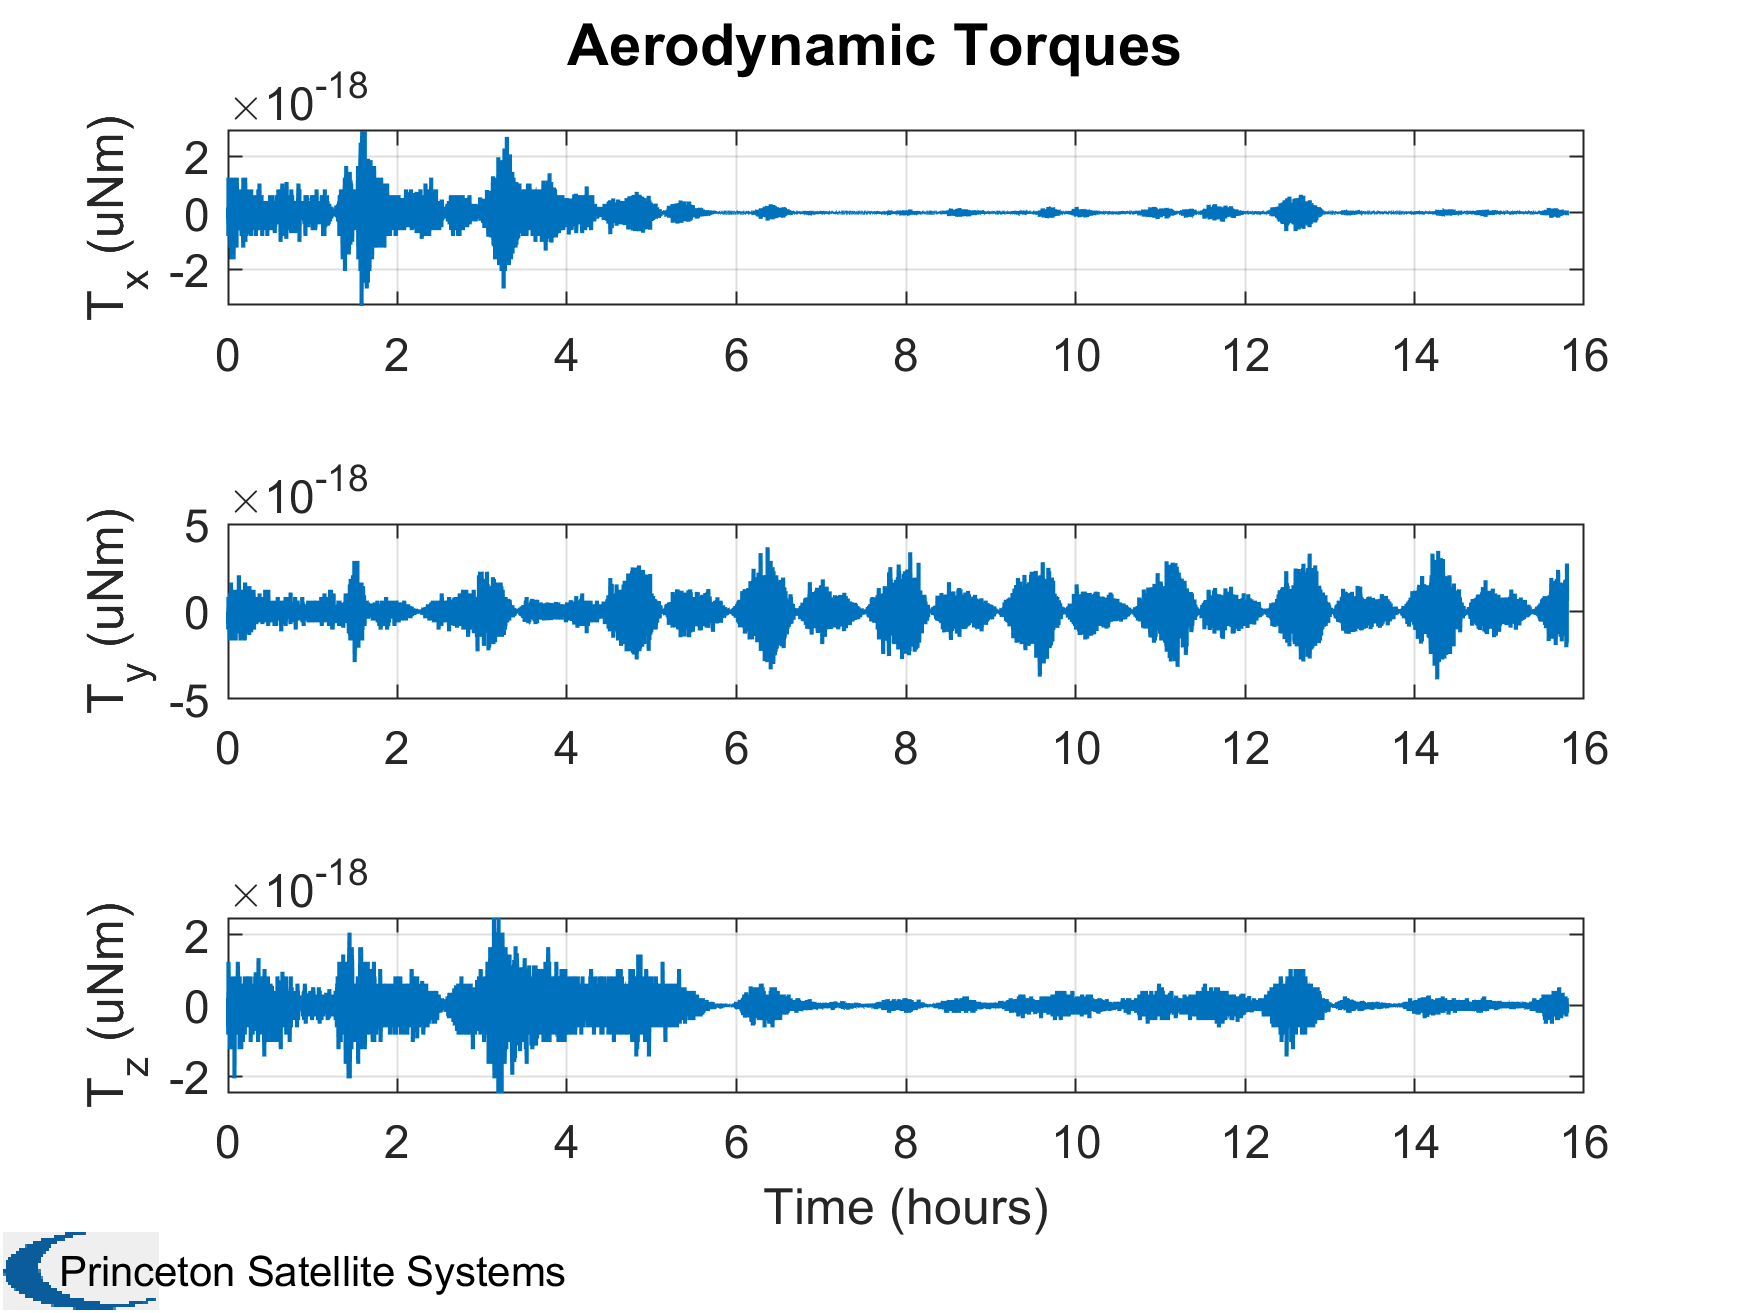
\includegraphics[width=0.95\linewidth]{res/img/Nadir_EKF/Simulations/Aerodynamic Torques.png}
            \caption{Aerodynamic Torques}
        \end{minipage}\hfill
        \begin{minipage}{0.48\linewidth}
            \centering
            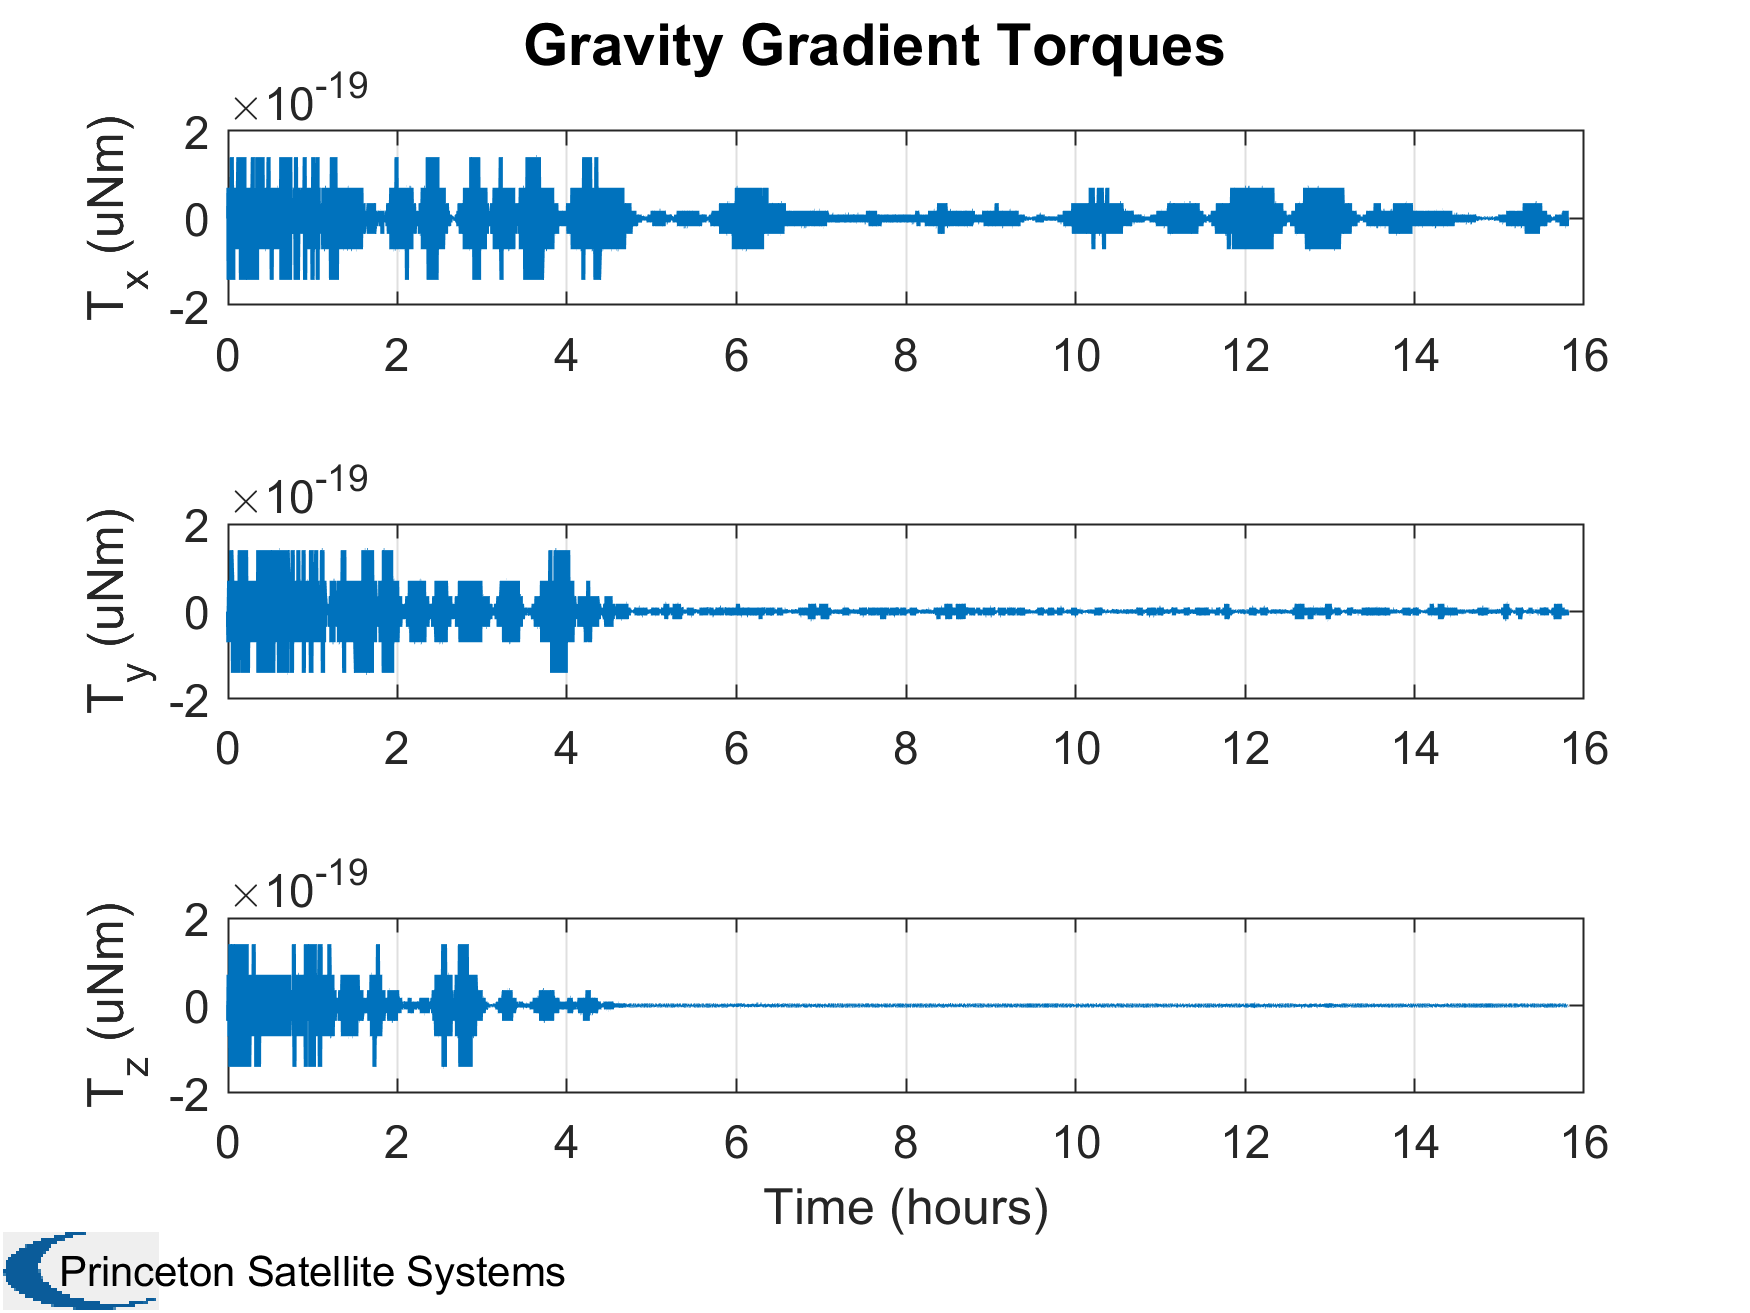
\includegraphics[width=0.95\linewidth]{res/img/Nadir_EKF/Simulations/Gravity Gradient Torques.png}
            \caption{Gravity Gradient Torques}
        \end{minipage}
    \end{figure}

    \begin{figure}[H]
        \centering
        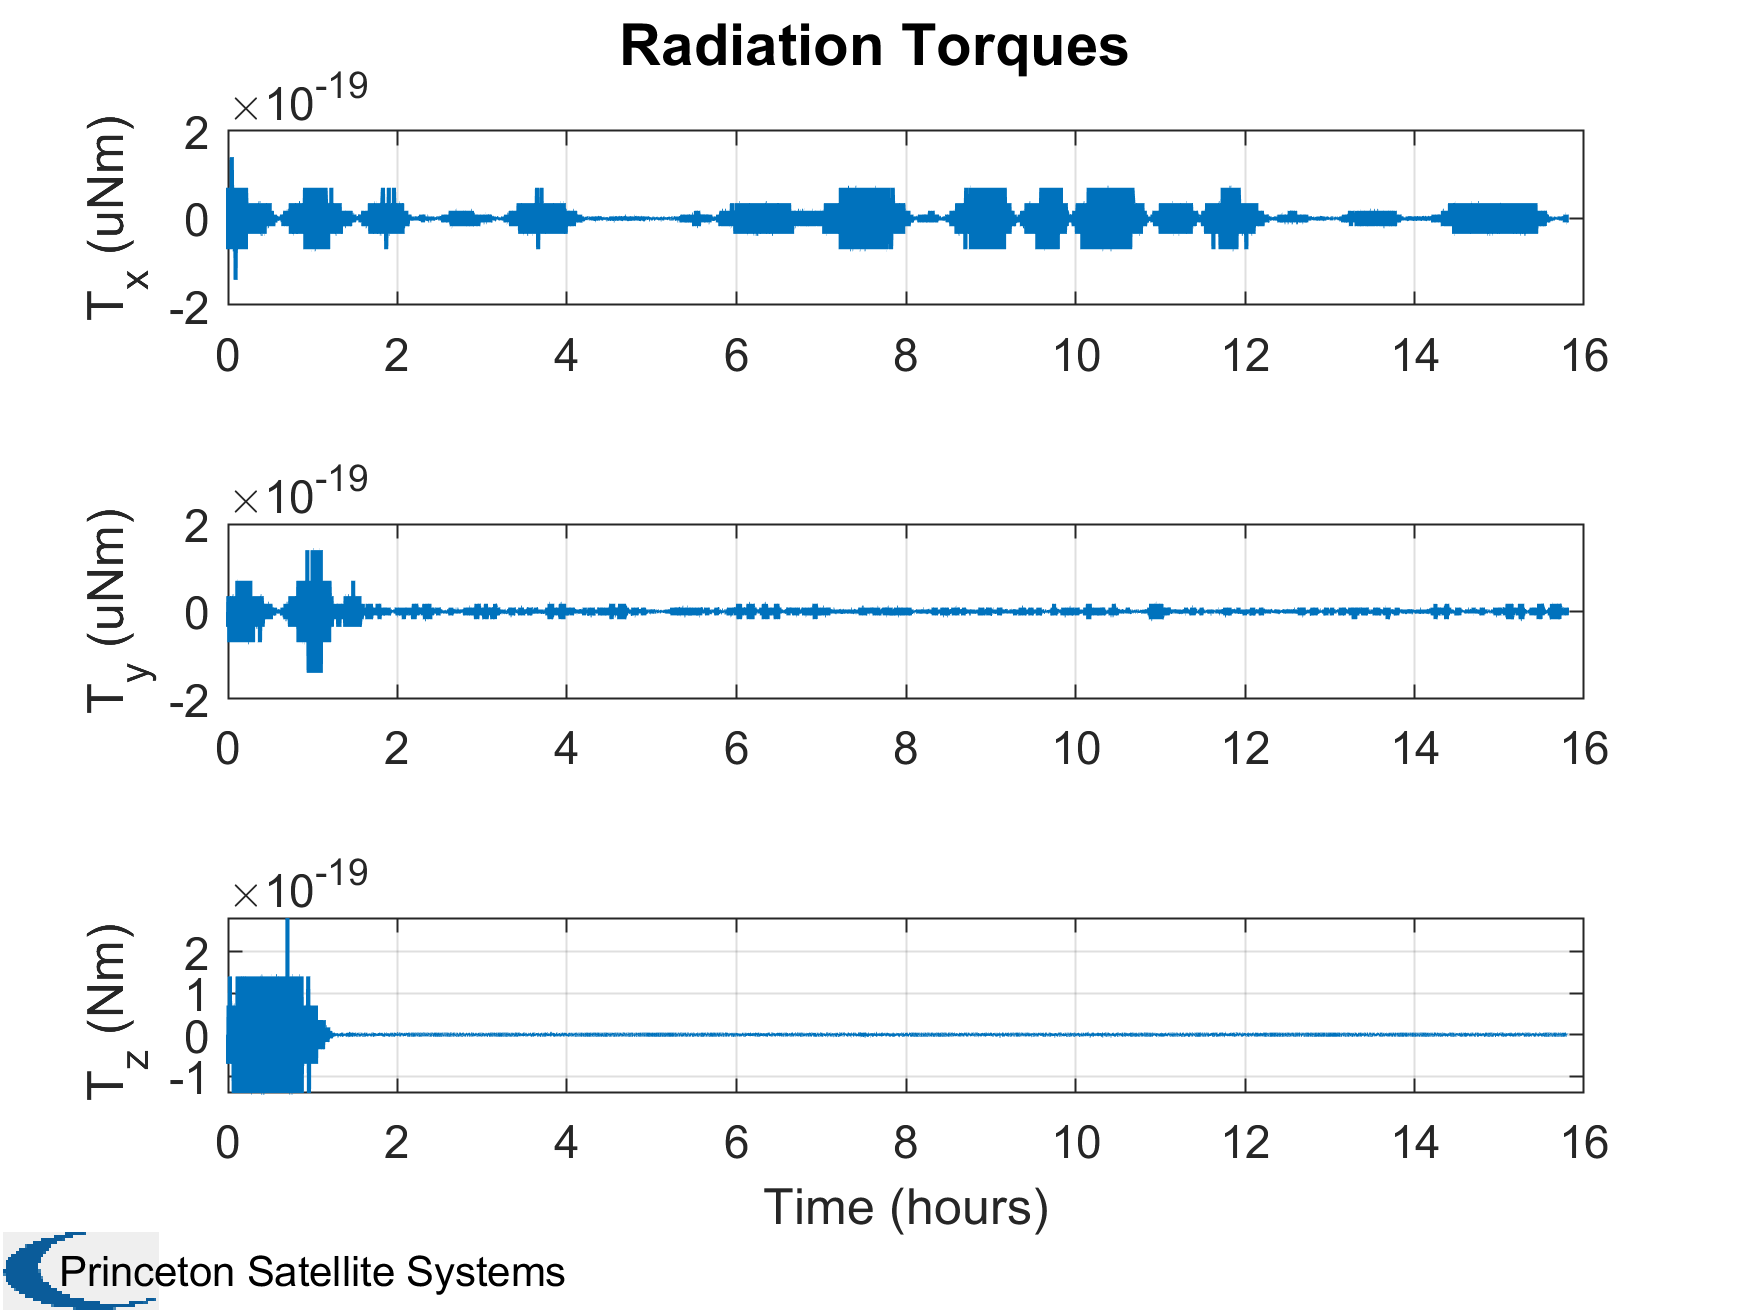
\includegraphics[width=0.48\linewidth]{res/img/Nadir_EKF/Simulations/Radiation Torques.png}
        \caption{Radiation Torques}
    \end{figure}

    \item \textbf{Sensor measurements}\\
    In this sectiona s in the previous simulation, the sensor measurements are presented. Firstly, the 
    gyroscope measurements are shown.
    \begin{figure}[H]
        \centering
        \begin{minipage}{0.32\linewidth}
            \centering
            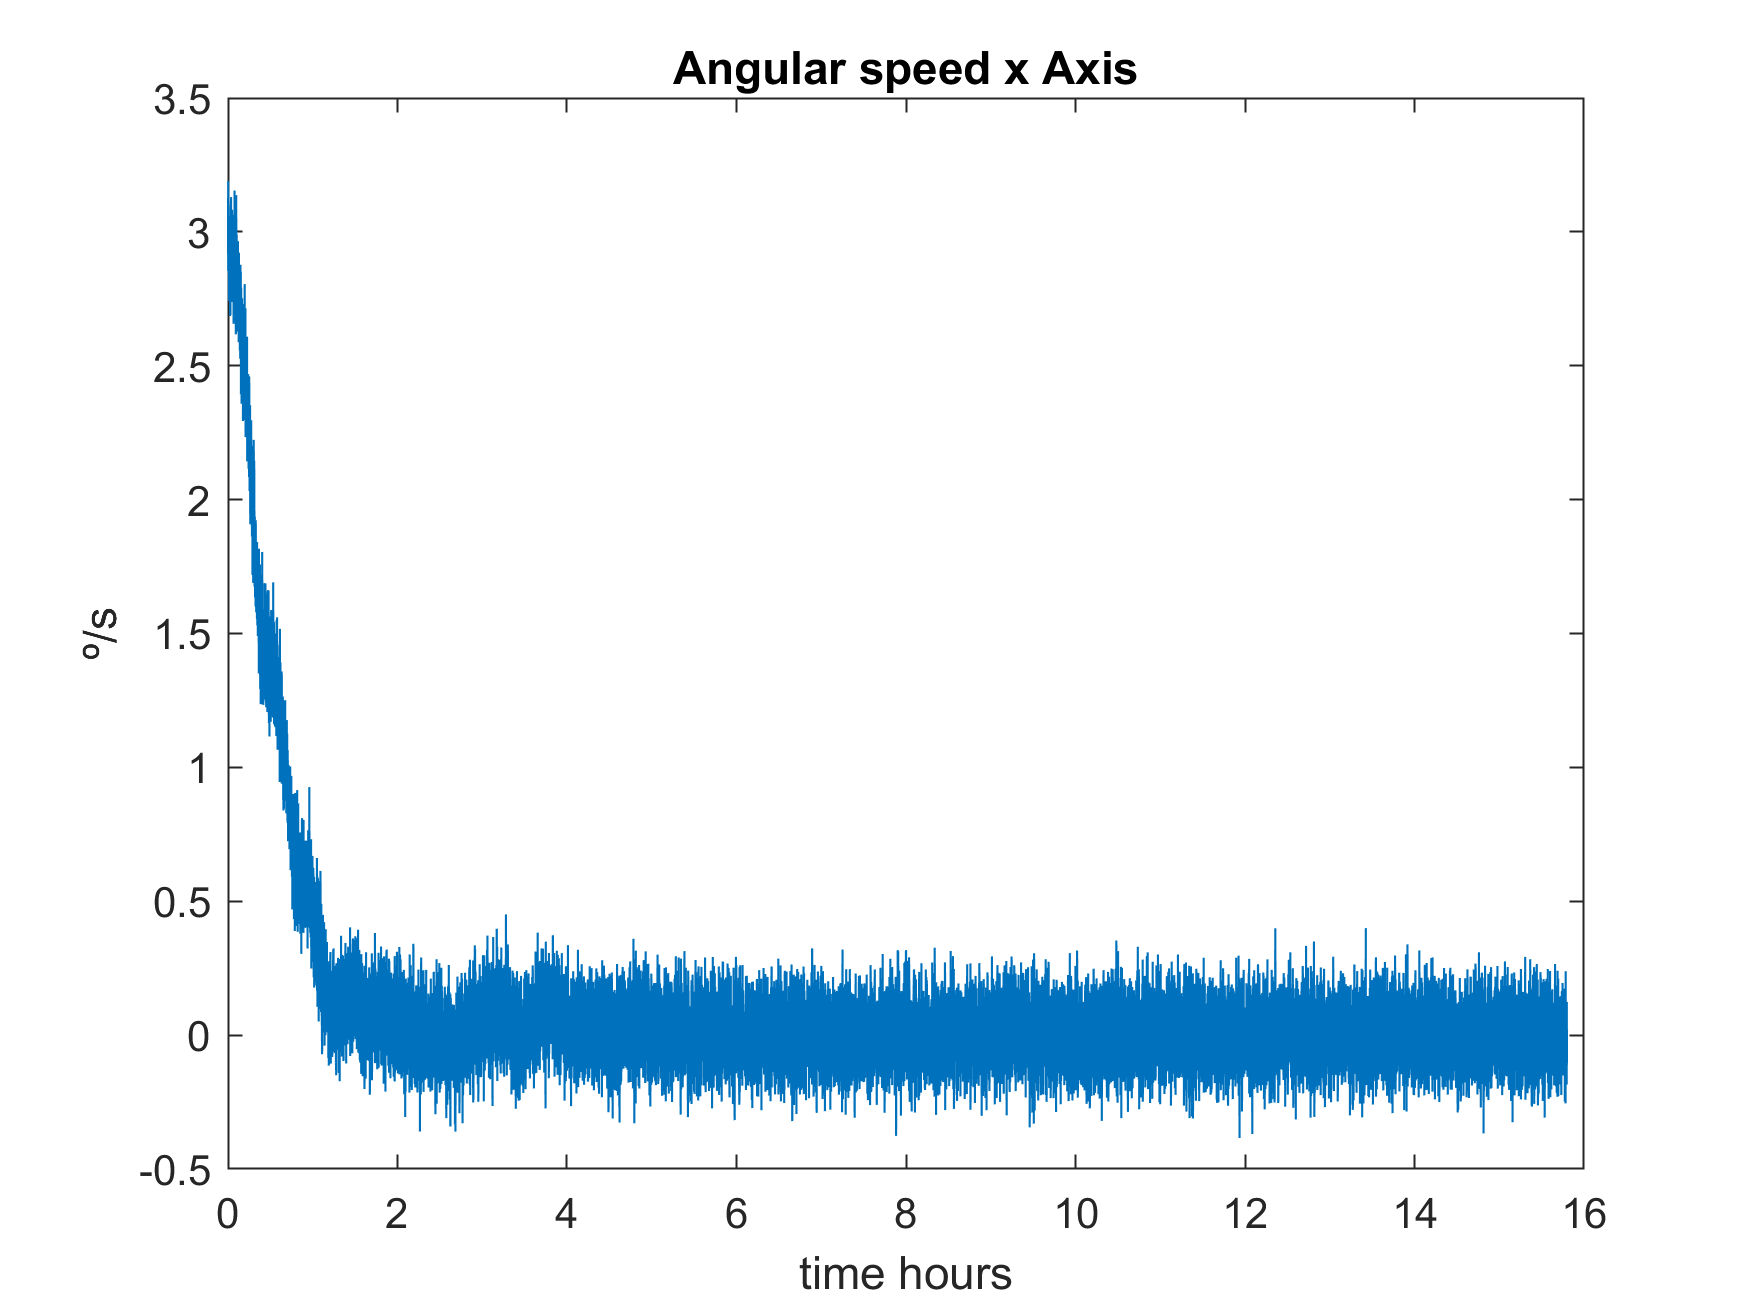
\includegraphics[width=0.95\linewidth]{res/img/Nadir_EKF/Simulations/Gyro data X Axis.png}
            \caption{Gyro data X Axis}
            \label{fig:GyroDataX}
        \end{minipage}\hfill
        \begin{minipage}{0.32\linewidth}
            \centering
            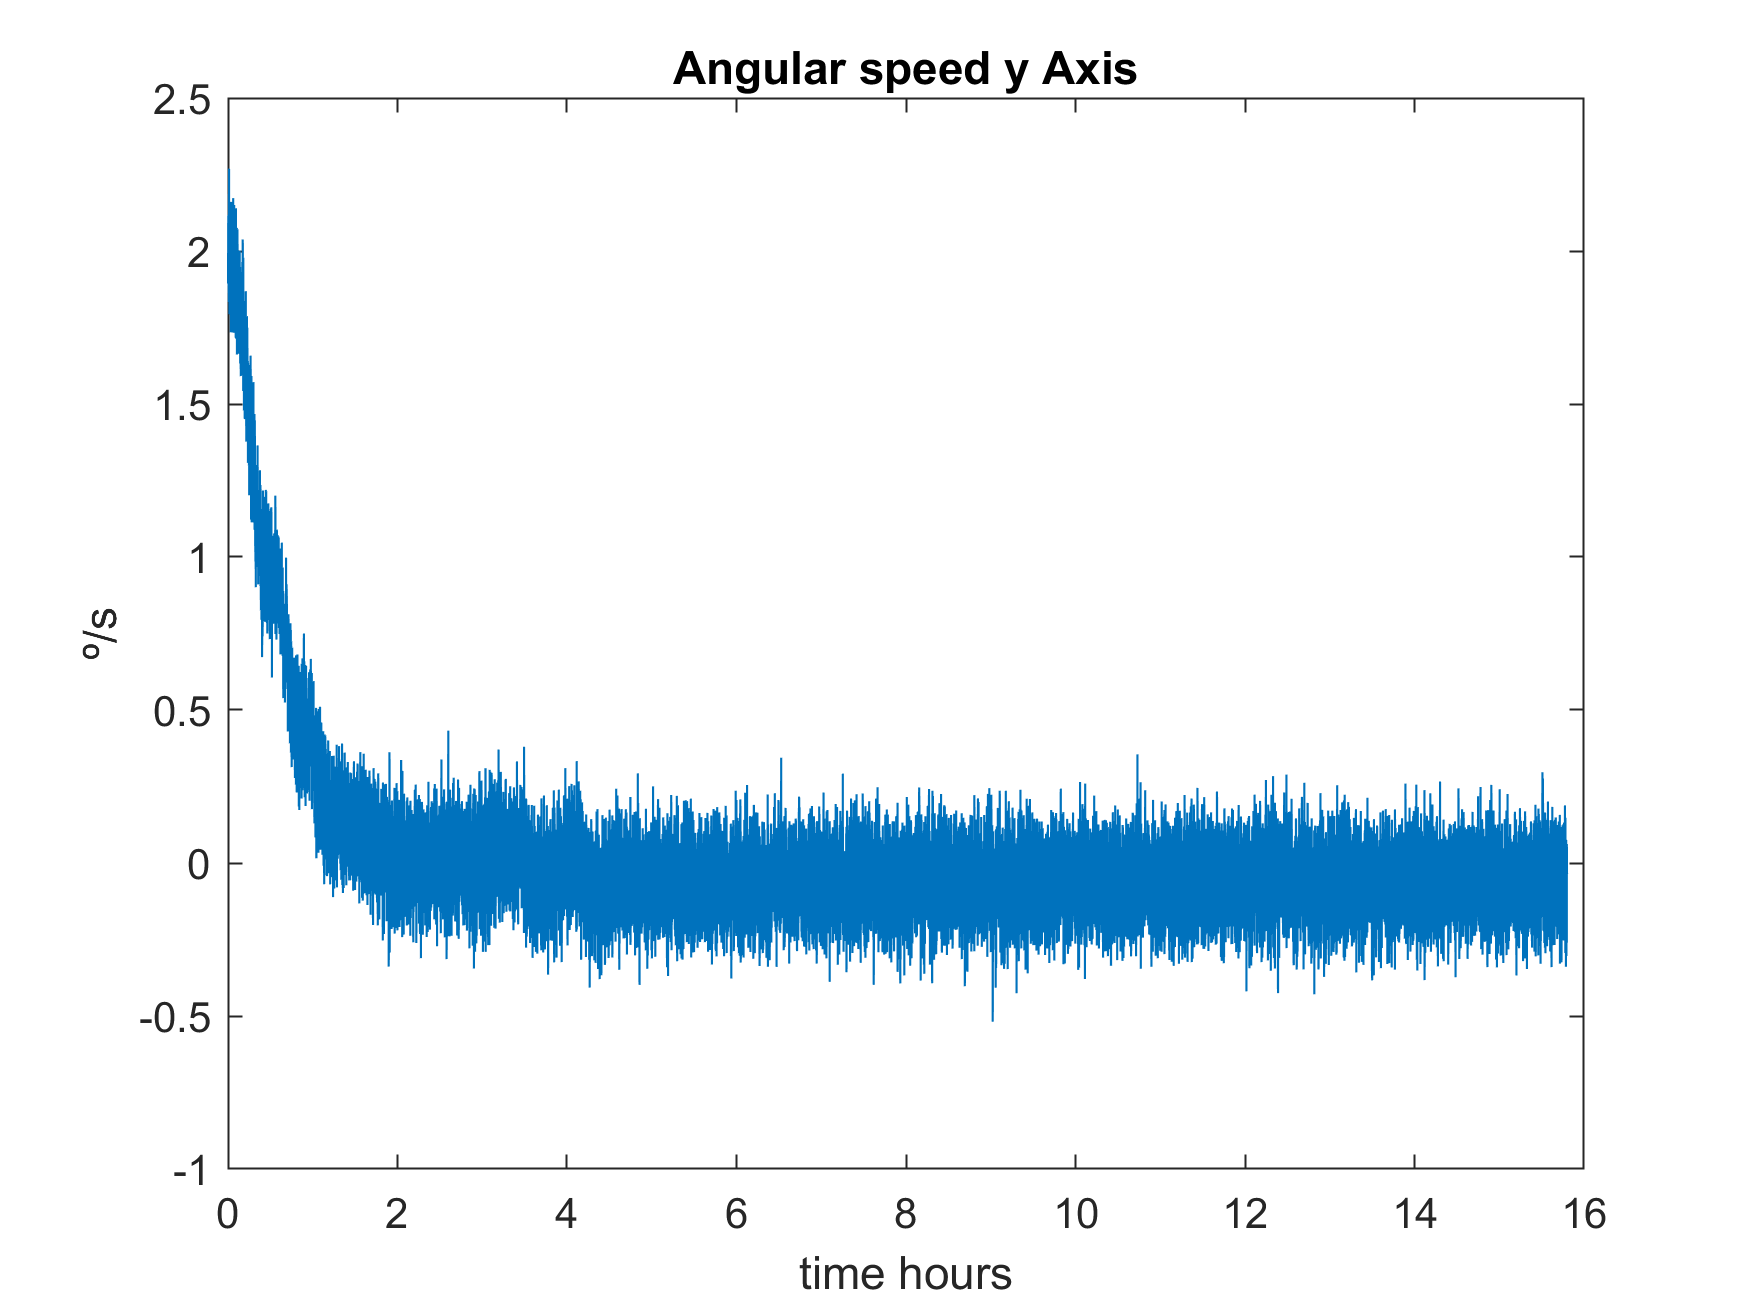
\includegraphics[width=0.95\linewidth]{res/img/Nadir_EKF/Simulations/Gyro data Y Axis.png}
            \caption{Gyro data Y Axis}
            \label{fig:GyroDataY}
        \end{minipage}\hfill
        \begin{minipage}{0.32\linewidth}
            \centering
            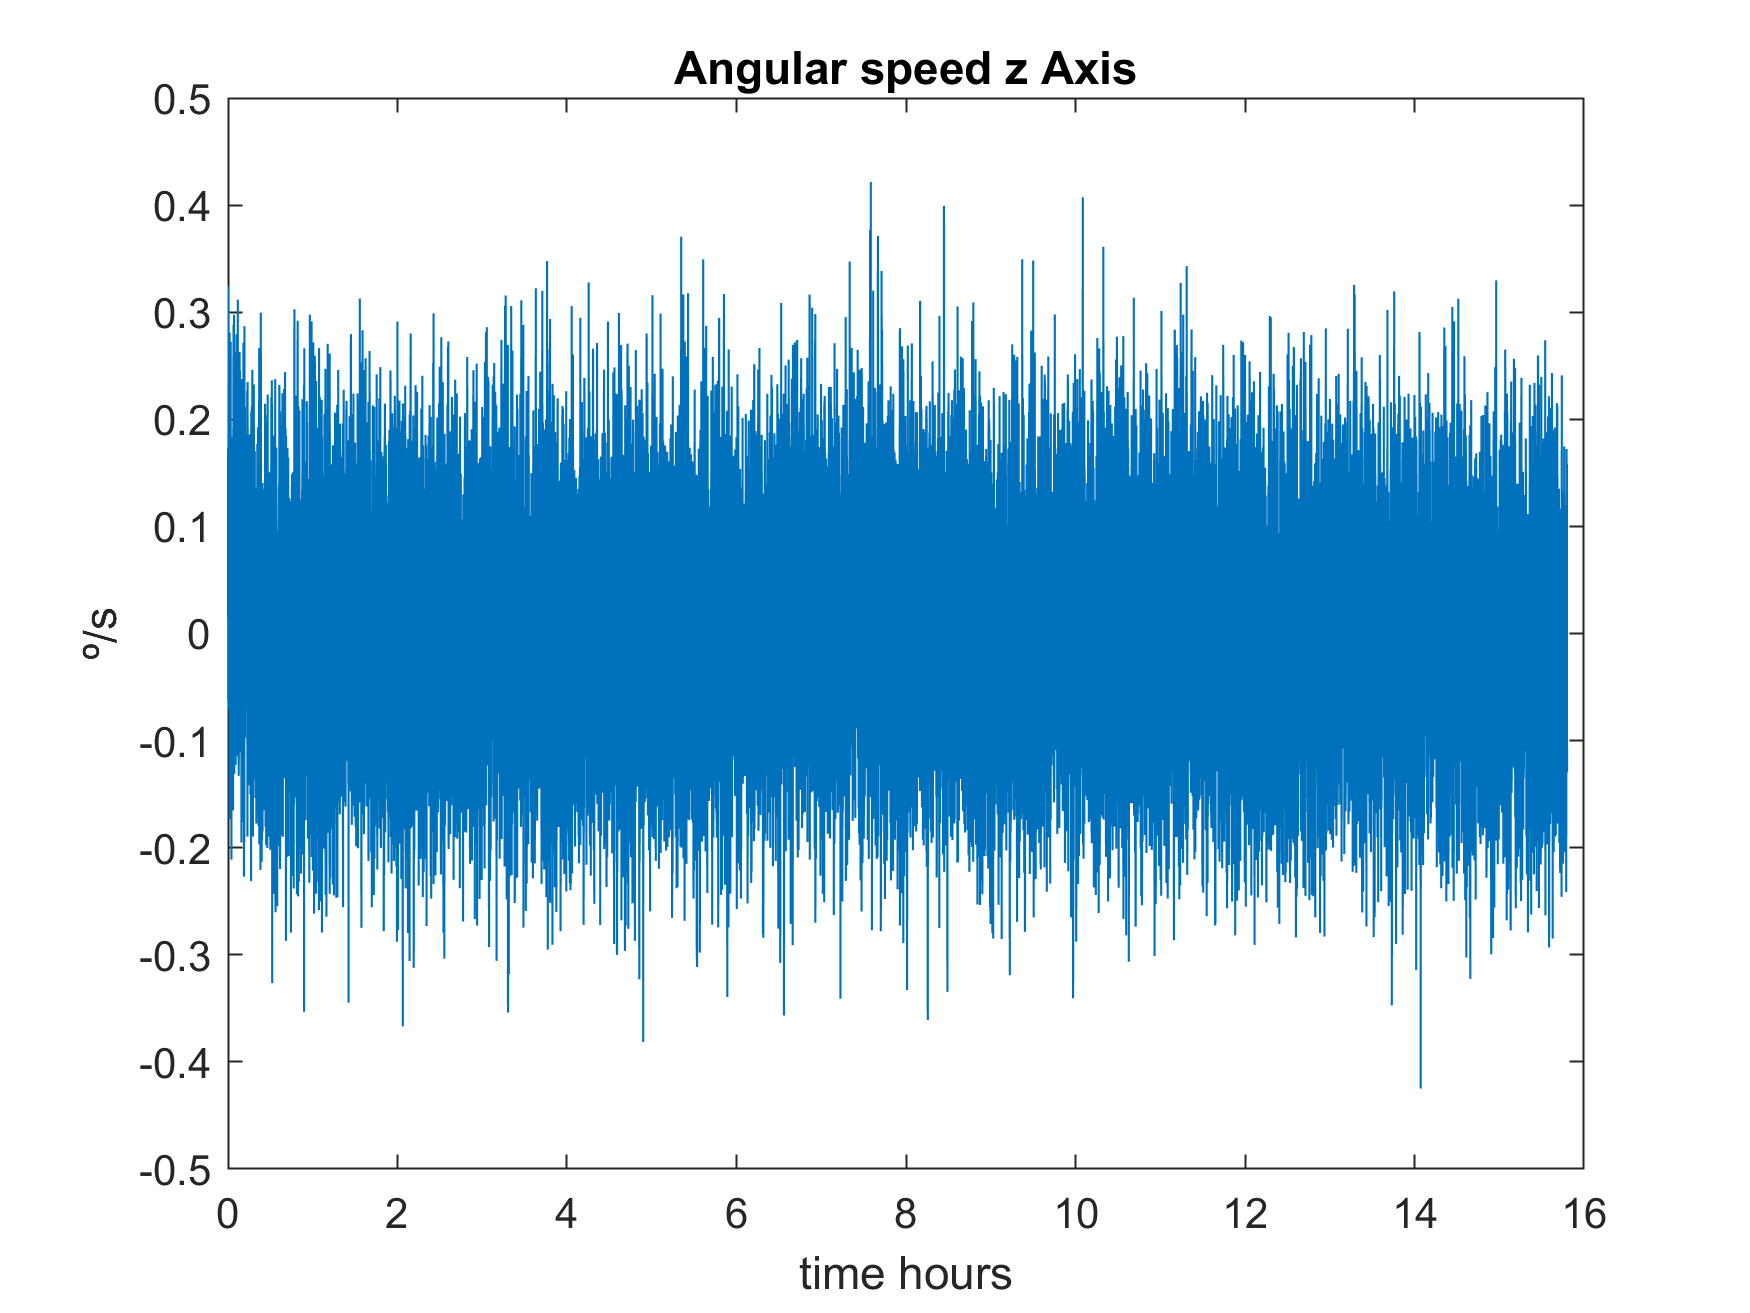
\includegraphics[width=0.95\linewidth]{res/img/Nadir_EKF/Simulations/Gyro data Z Axis.png}
            \caption{Gyro data Z Axis}
            \label{fig:GyroDataZ}
        \end{minipage}
    \end{figure}

    Secondly, the magnetometer measurements are presented.
    \begin{figure}[H]
        \centering
        \begin{minipage}{0.32\linewidth}
            \centering
            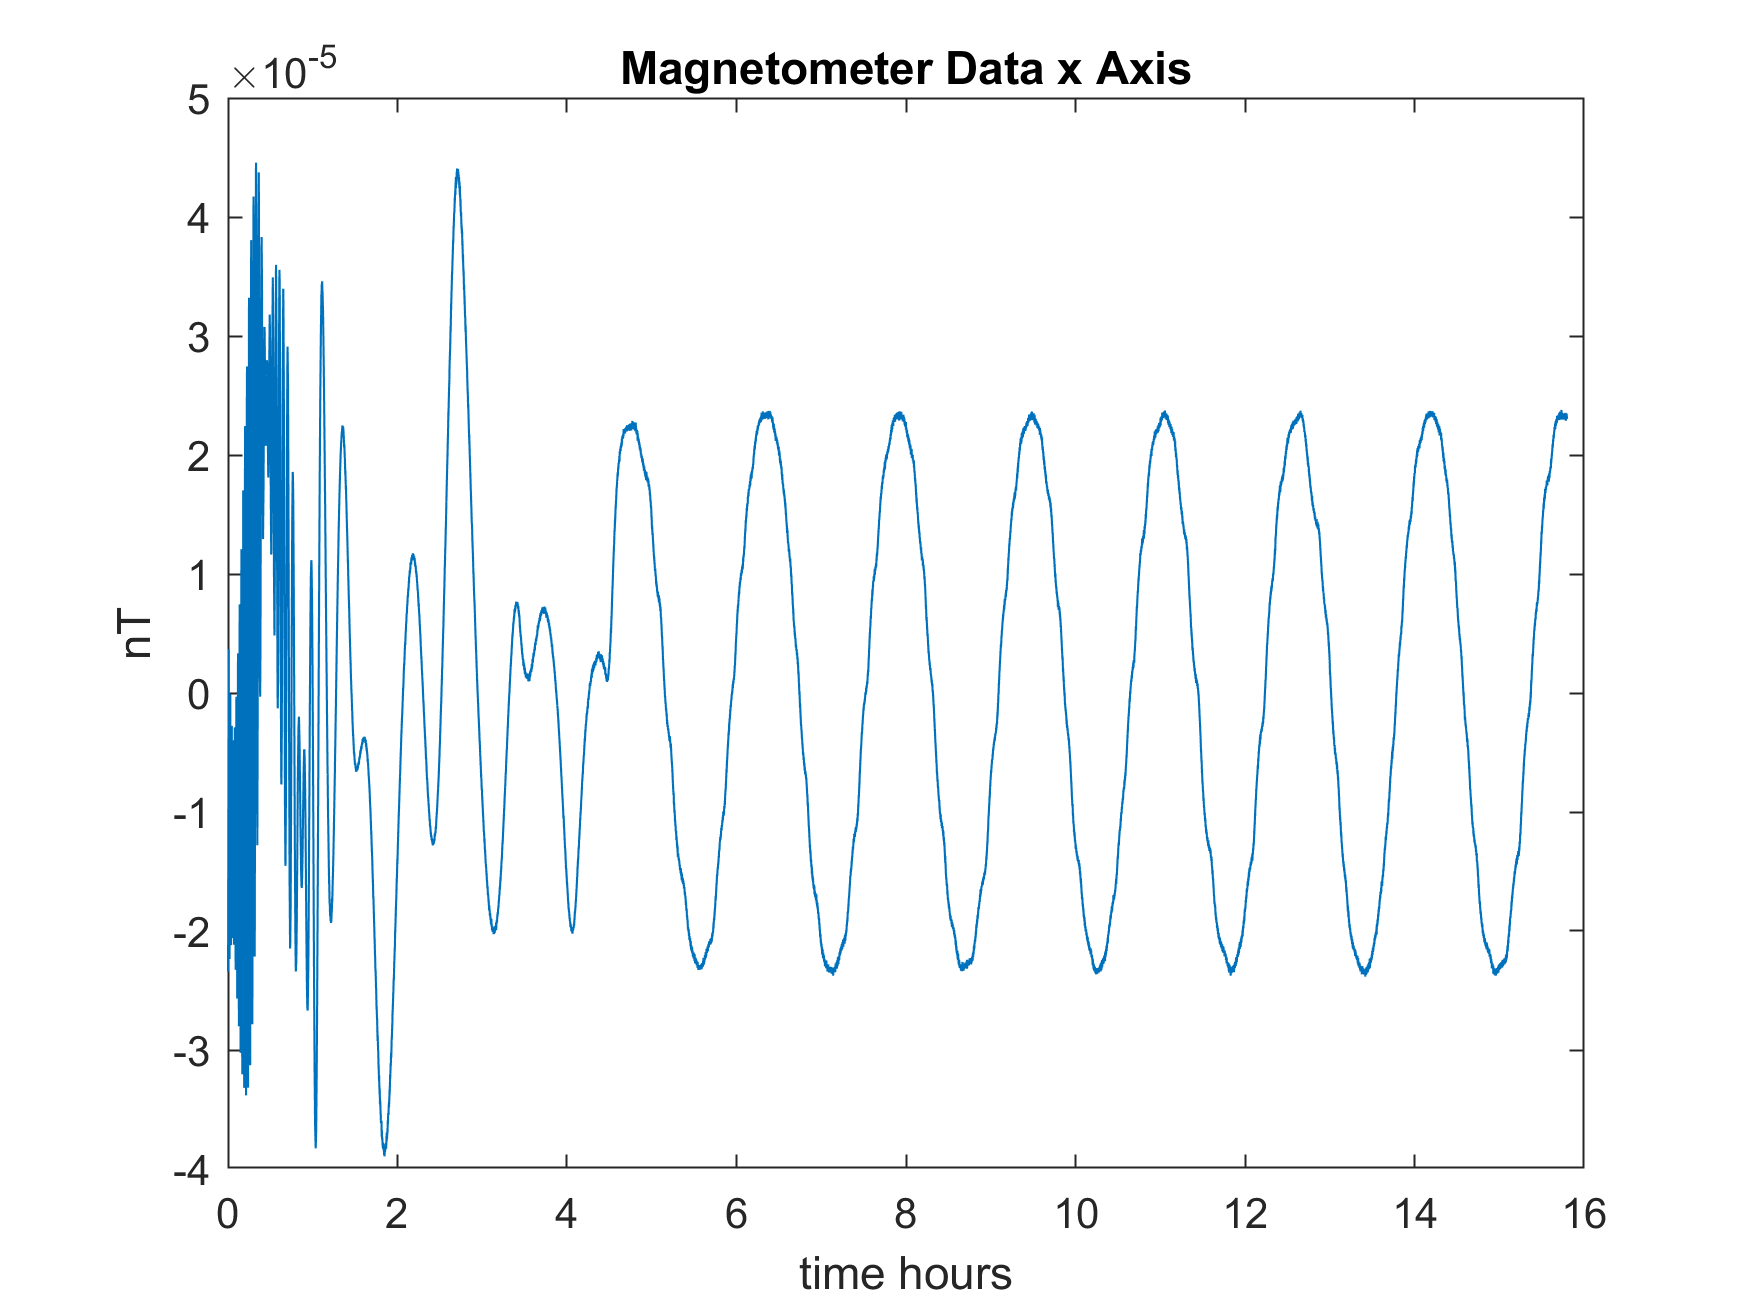
\includegraphics[width=0.95\linewidth]{res/img/Nadir_EKF/Simulations/Magnetometer data X Axis.png}
            \caption{Magnetometer data X Axis}
            \label{fig:MagnetometerDataX}
        \end{minipage}\hfill
        \begin{minipage}{0.32\linewidth}
            \centering
            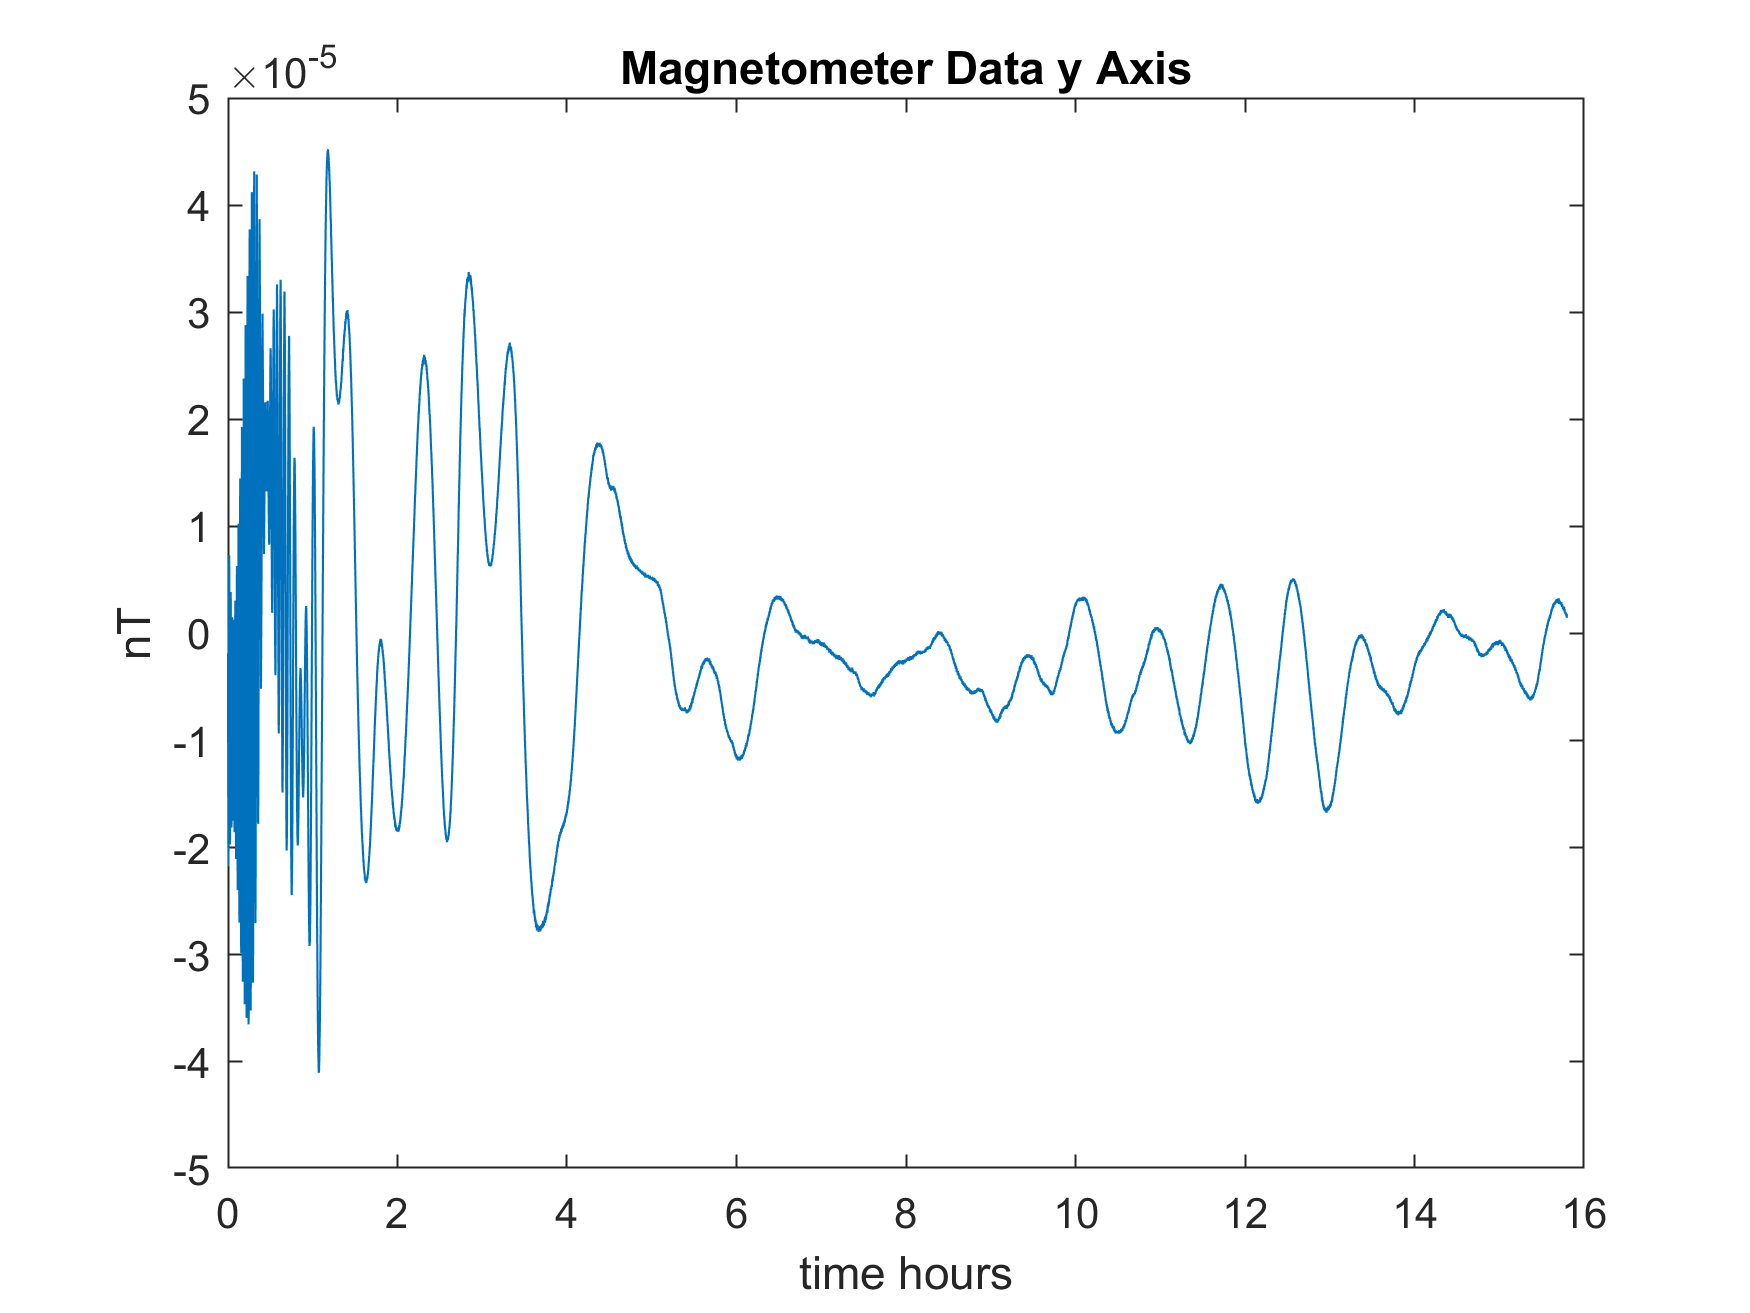
\includegraphics[width=0.95\linewidth]{res/img/Nadir_EKF/Simulations/Magnetometer data Y Axis.png}
            \caption{Magnetometer data Y Axis}
            \label{fig:MagnetometerDataY}
        \end{minipage}\hfill
        \begin{minipage}{0.32\linewidth}
            \centering
            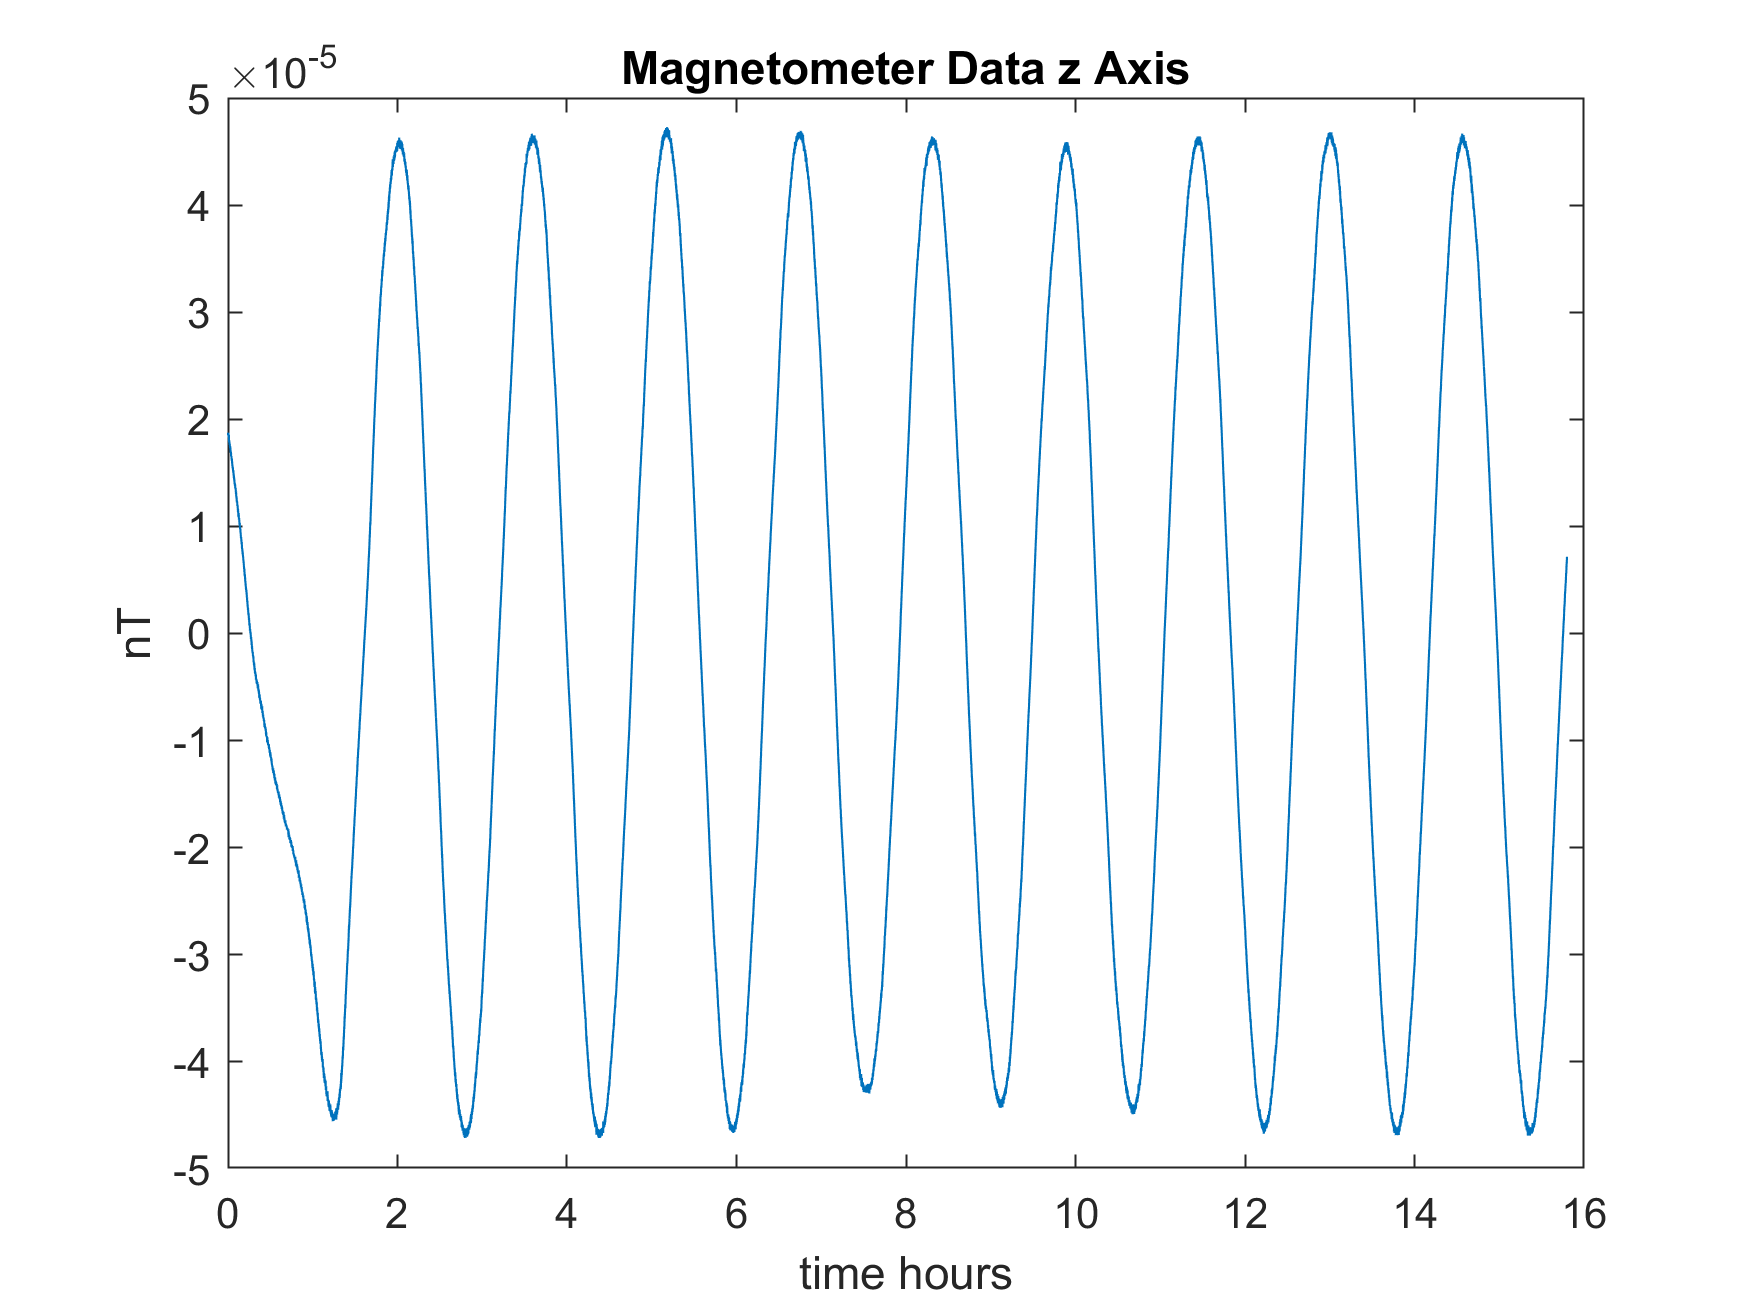
\includegraphics[width=0.95\linewidth]{res/img/Nadir_EKF/Simulations/Magnetometer data Z Axis.png}
            \caption{Magnetometer data Z Axis}
            \label{fig:MagnetometerDataZ}
        \end{minipage}
    \end{figure}

    Finally, the photodiode measurements are presented. As in the previous simulation, each axis of the PQ corresponds to the following number: 1 to +Z, 2 to -Z, 3 to +X, 4 to +Y,
    5 to -X and 6 to -Y.
    \begin{figure}[H]
        \centering
        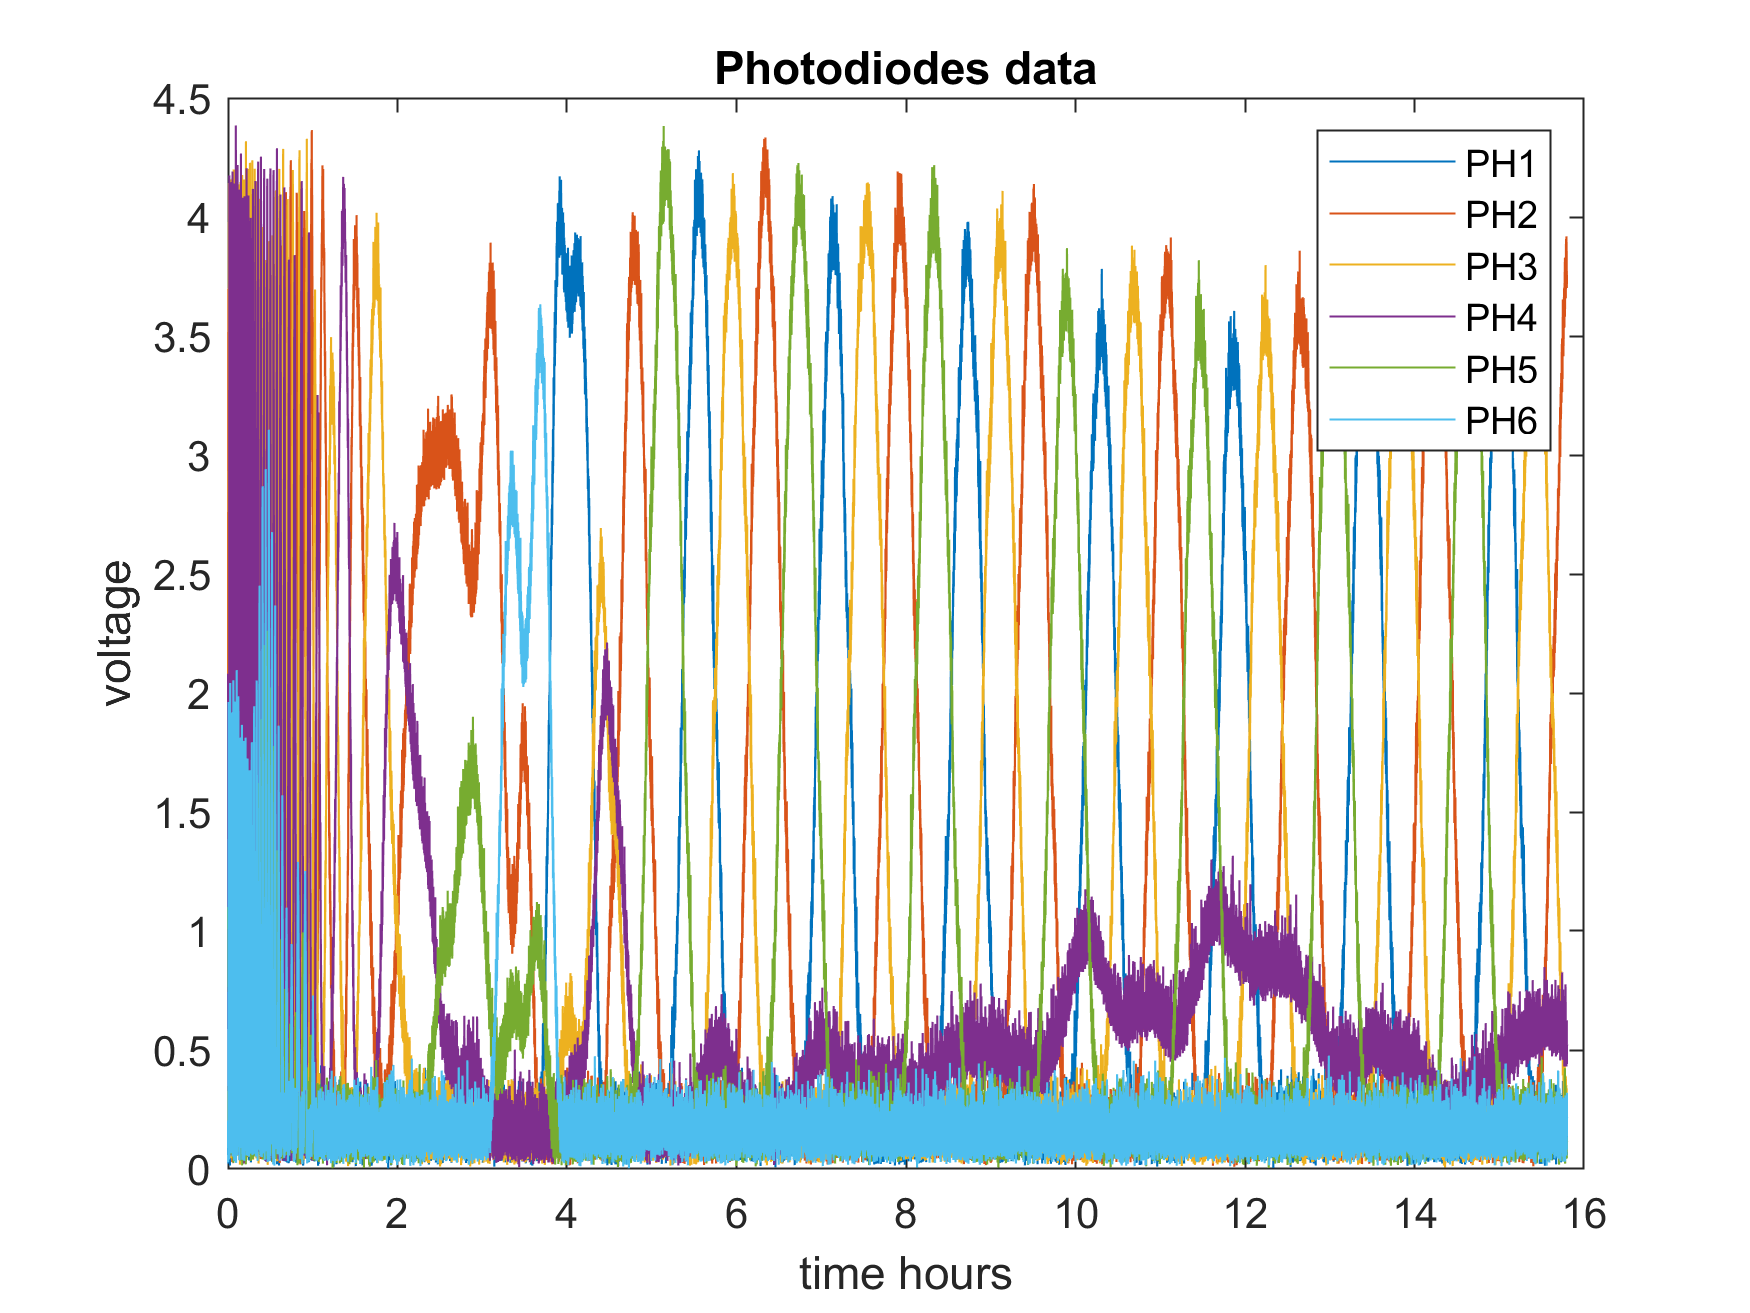
\includegraphics[width=0.7\linewidth]{res/img/Nadir_EKF/Simulations/Photodiode data.png}
        \caption{Photodiode data}
        \label{fig:PhotodiodeData}
    \end{figure}

    \item \textbf{Sun Position Algorithm Performance}\\
    In this section the performance of the developed Sun position algorithm estimator that uses the photodiodes and the temperature sensors is presented. Remember that
    the orange line indicates the real position of the sun, and the blue line indicates the estimation of the algorithm. 
    \begin{figure}[H]
        \centering
        \begin{minipage}{0.32\linewidth}
            \centering
            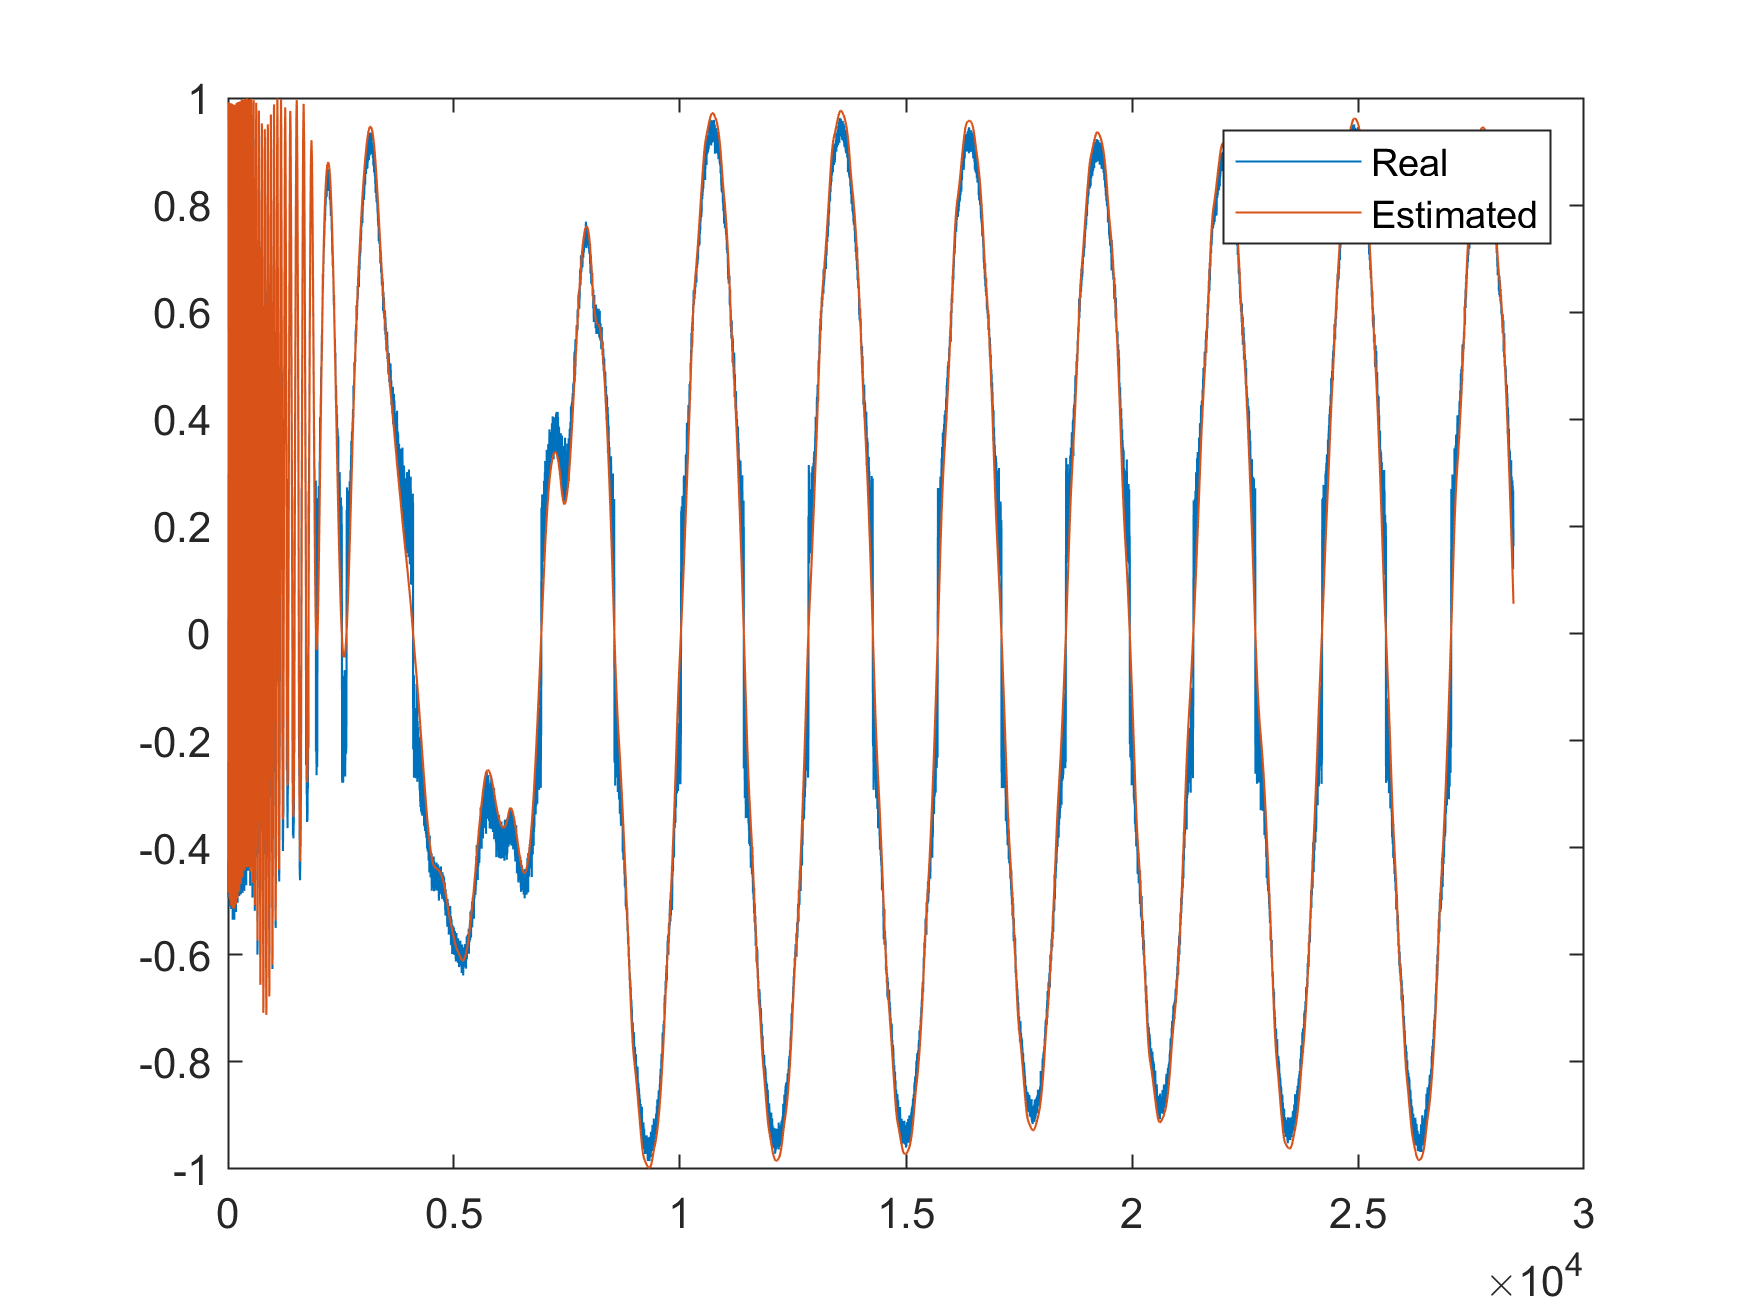
\includegraphics[width=0.95\linewidth]{res/img/Nadir_EKF/Simulations/Sun position (ECI) X Axis.png}
            \caption{Sun position (ECI) X Axis}
            \label{fig:SunPositionECIX}
        \end{minipage}\hfill
        \begin{minipage}{0.32\linewidth}
            \centering
            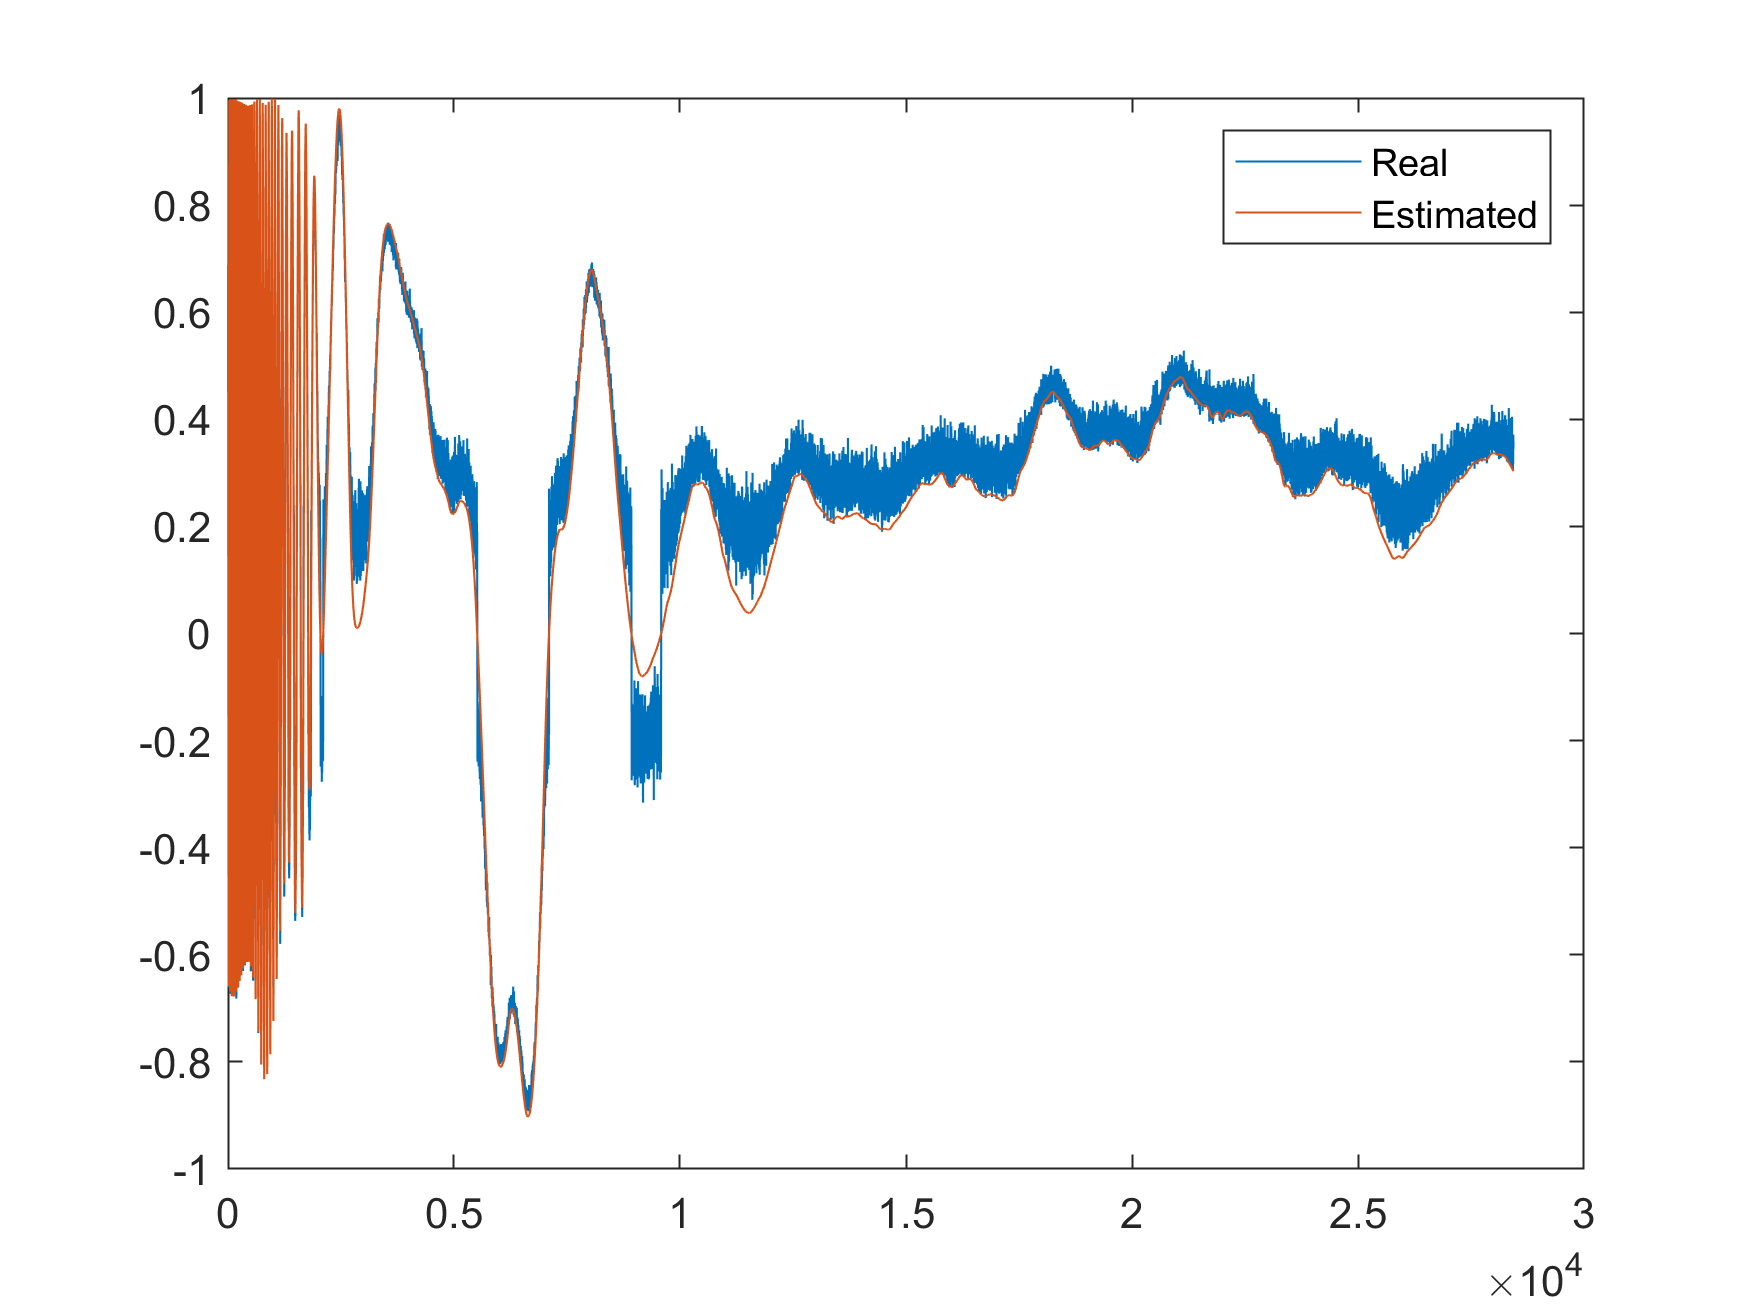
\includegraphics[width=0.95\linewidth]{res/img/Nadir_EKF/Simulations/Sun position (ECI) Y Axis.png}
            \caption{Sun position (ECI) Y Axis}
            \label{fig:SunPositionECIY}
        \end{minipage}\hfill
        \begin{minipage}{0.32\linewidth}
            \centering
            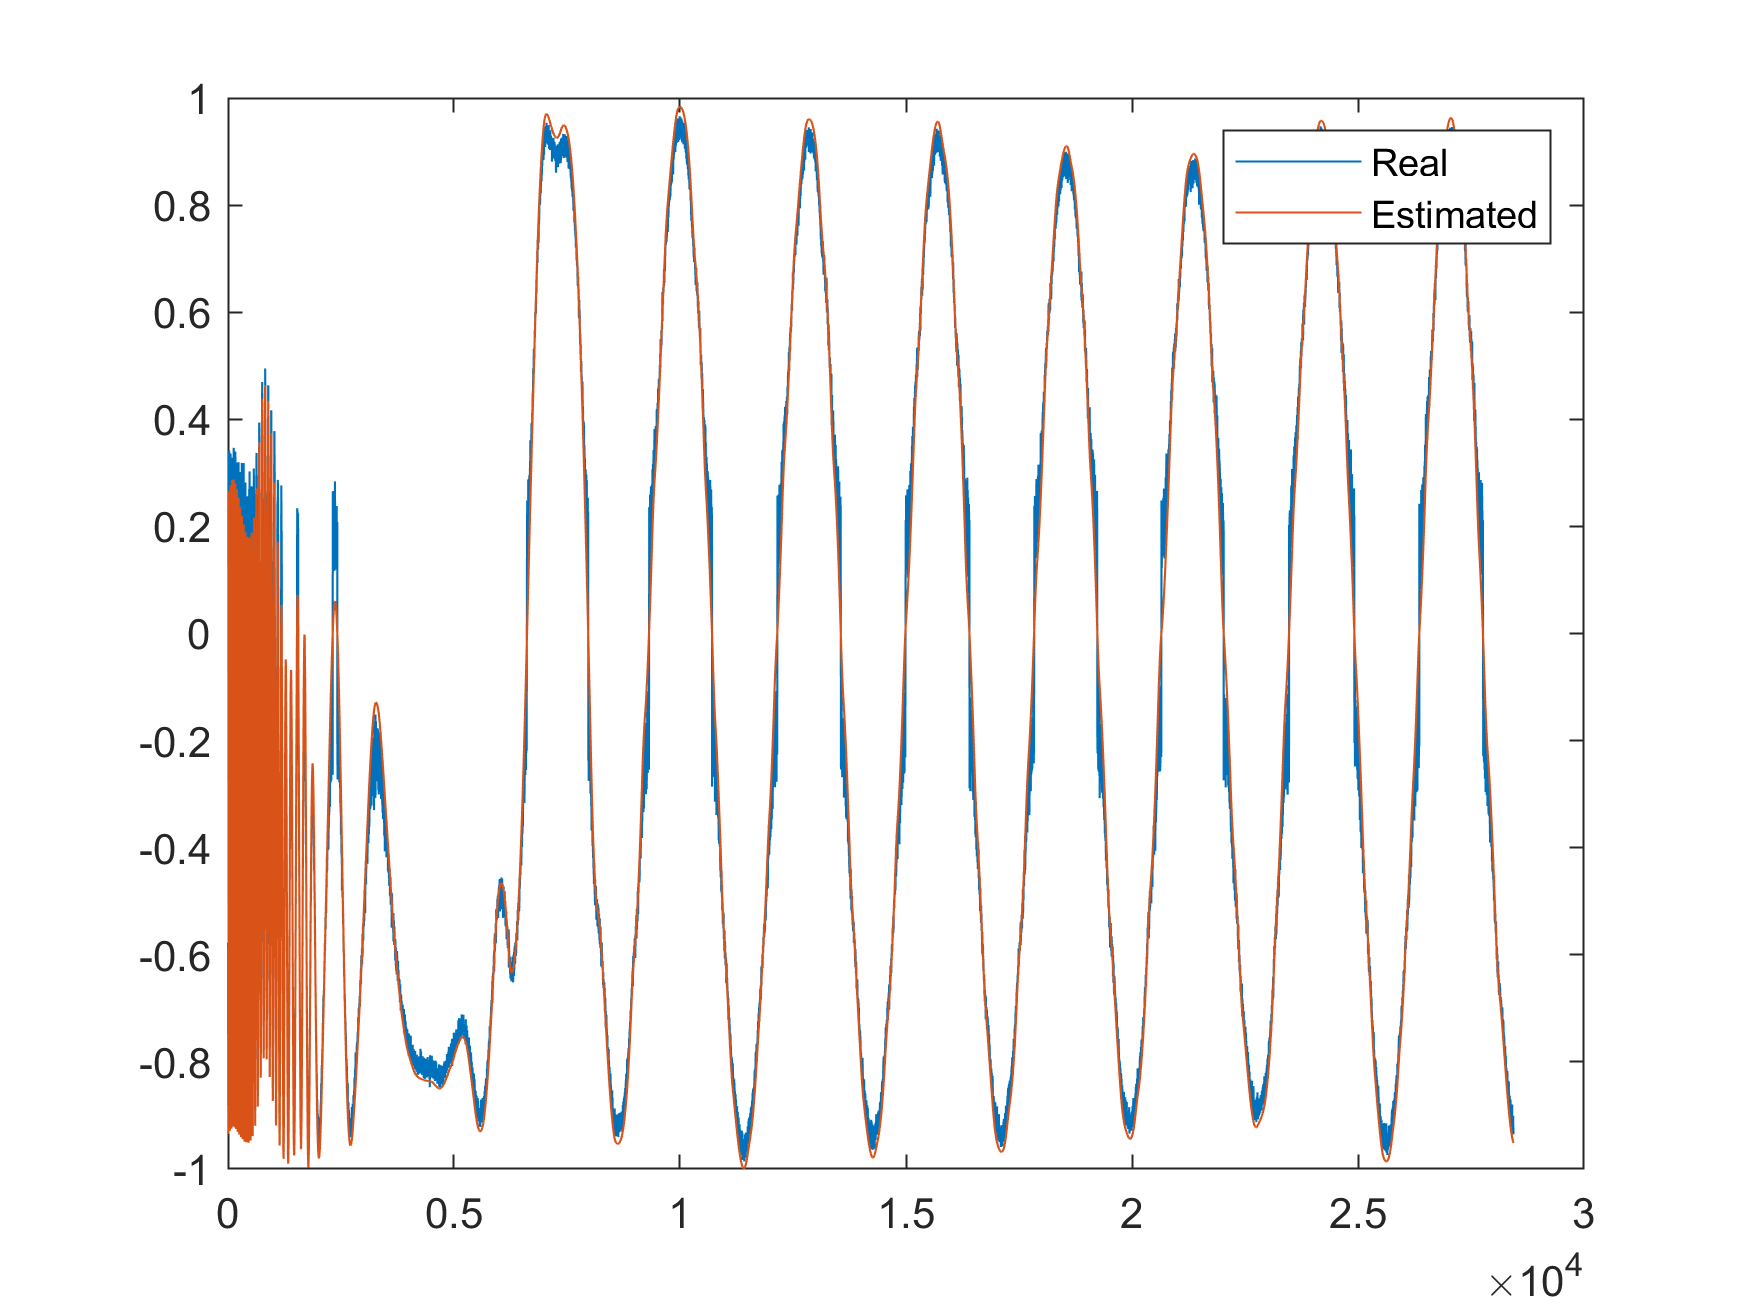
\includegraphics[width=0.95\linewidth]{res/img/Nadir_EKF/Simulations/Sun position (ECI) Z Axis.png}
            \caption{Sun position (ECI) Z Axis}
            \label{fig:SunPositionECIZ}
        \end{minipage}
    \end{figure}

    \item \textbf{Real angular Velocity}\\
    This section presents the angular velocity propagated in each iteration of the simulation.
    \begin{figure}[H]
        \centering
        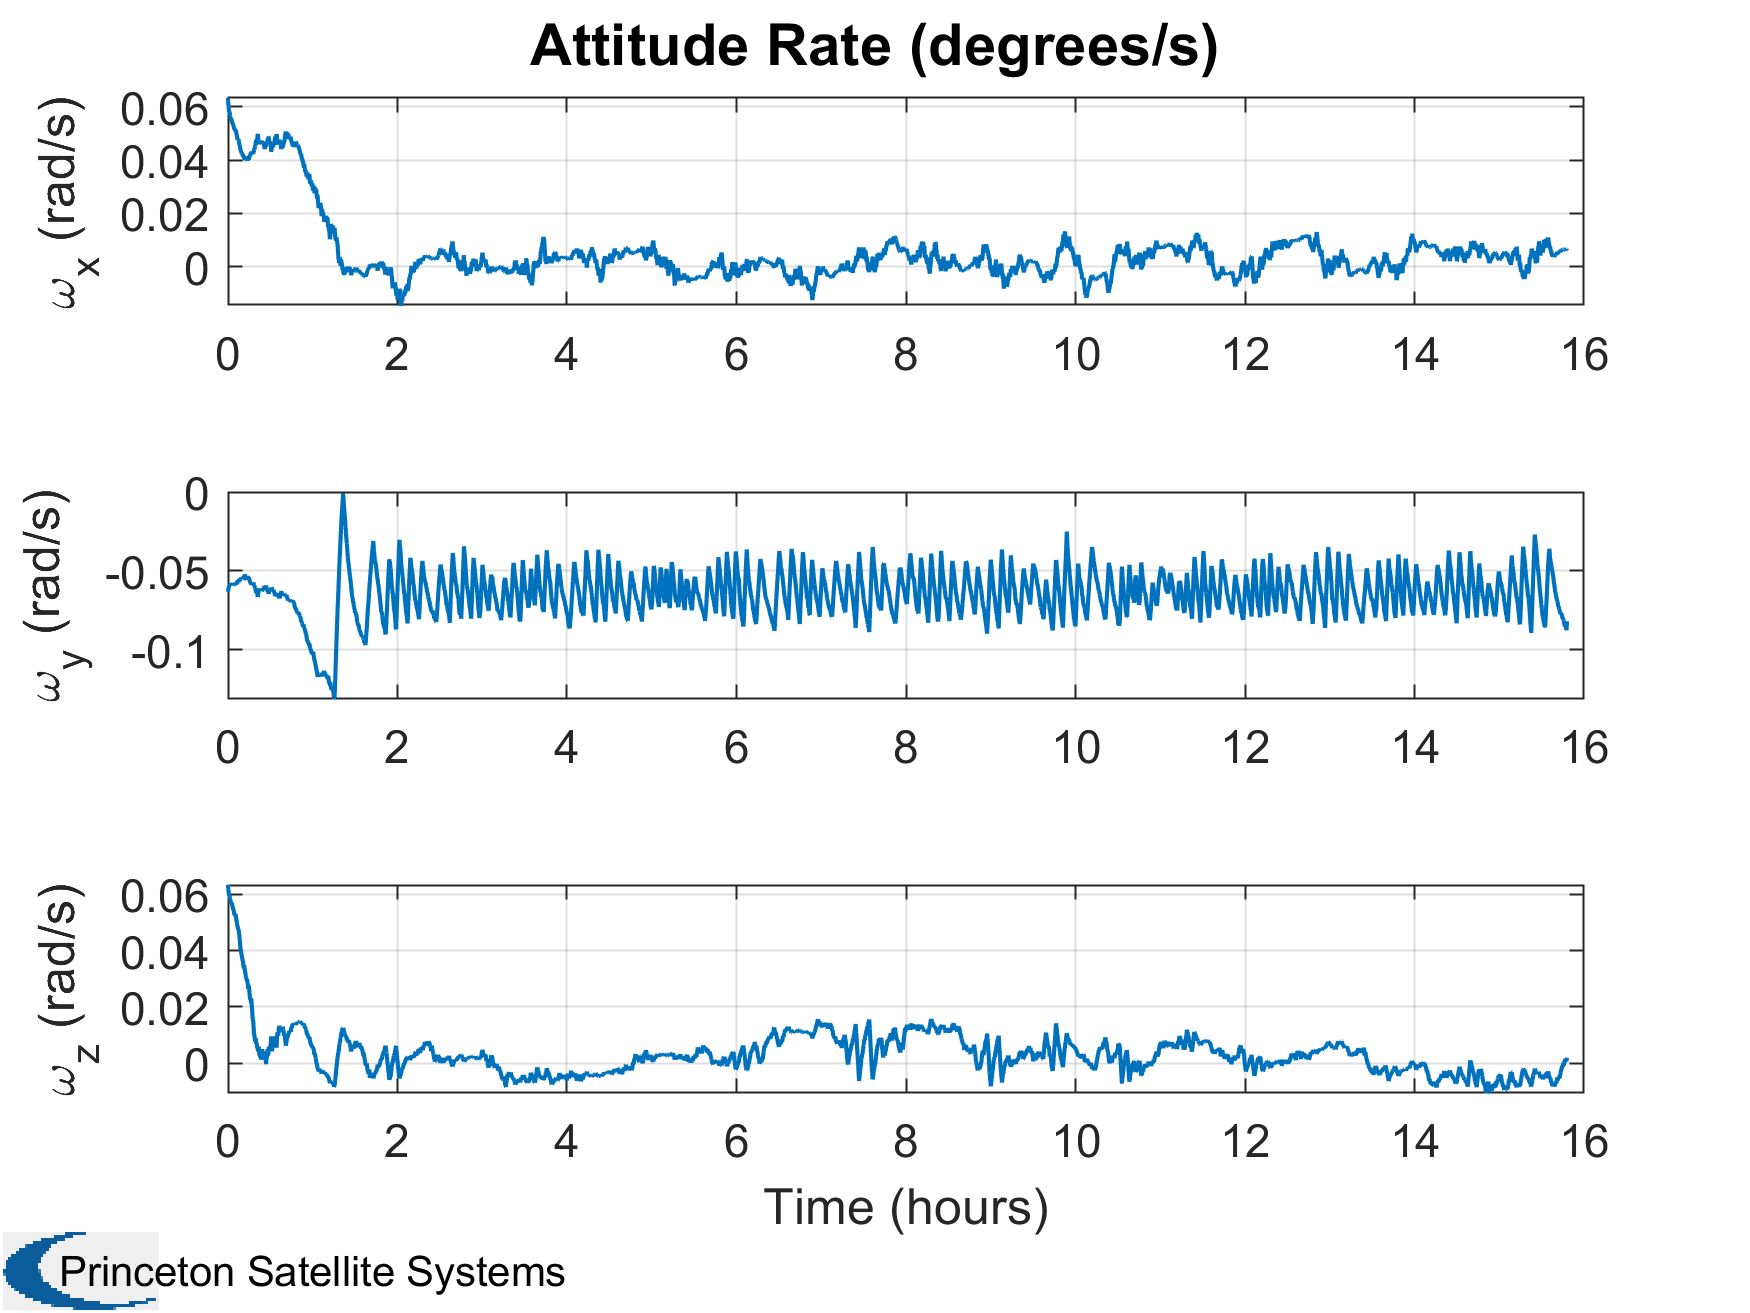
\includegraphics[width=0.5\linewidth]{res/img/Nadir_EKF/Simulations/Attitude Rate.png}
        \caption{Attitude Rate}
        \label{fig:AttitudeRate}
    \end{figure}

    \item \textbf{Generated torque}\\
    The following plot shows the generated torque by the magnetic moment generated by the magnetorquers.
    \begin{figure}[H]
        \centering
        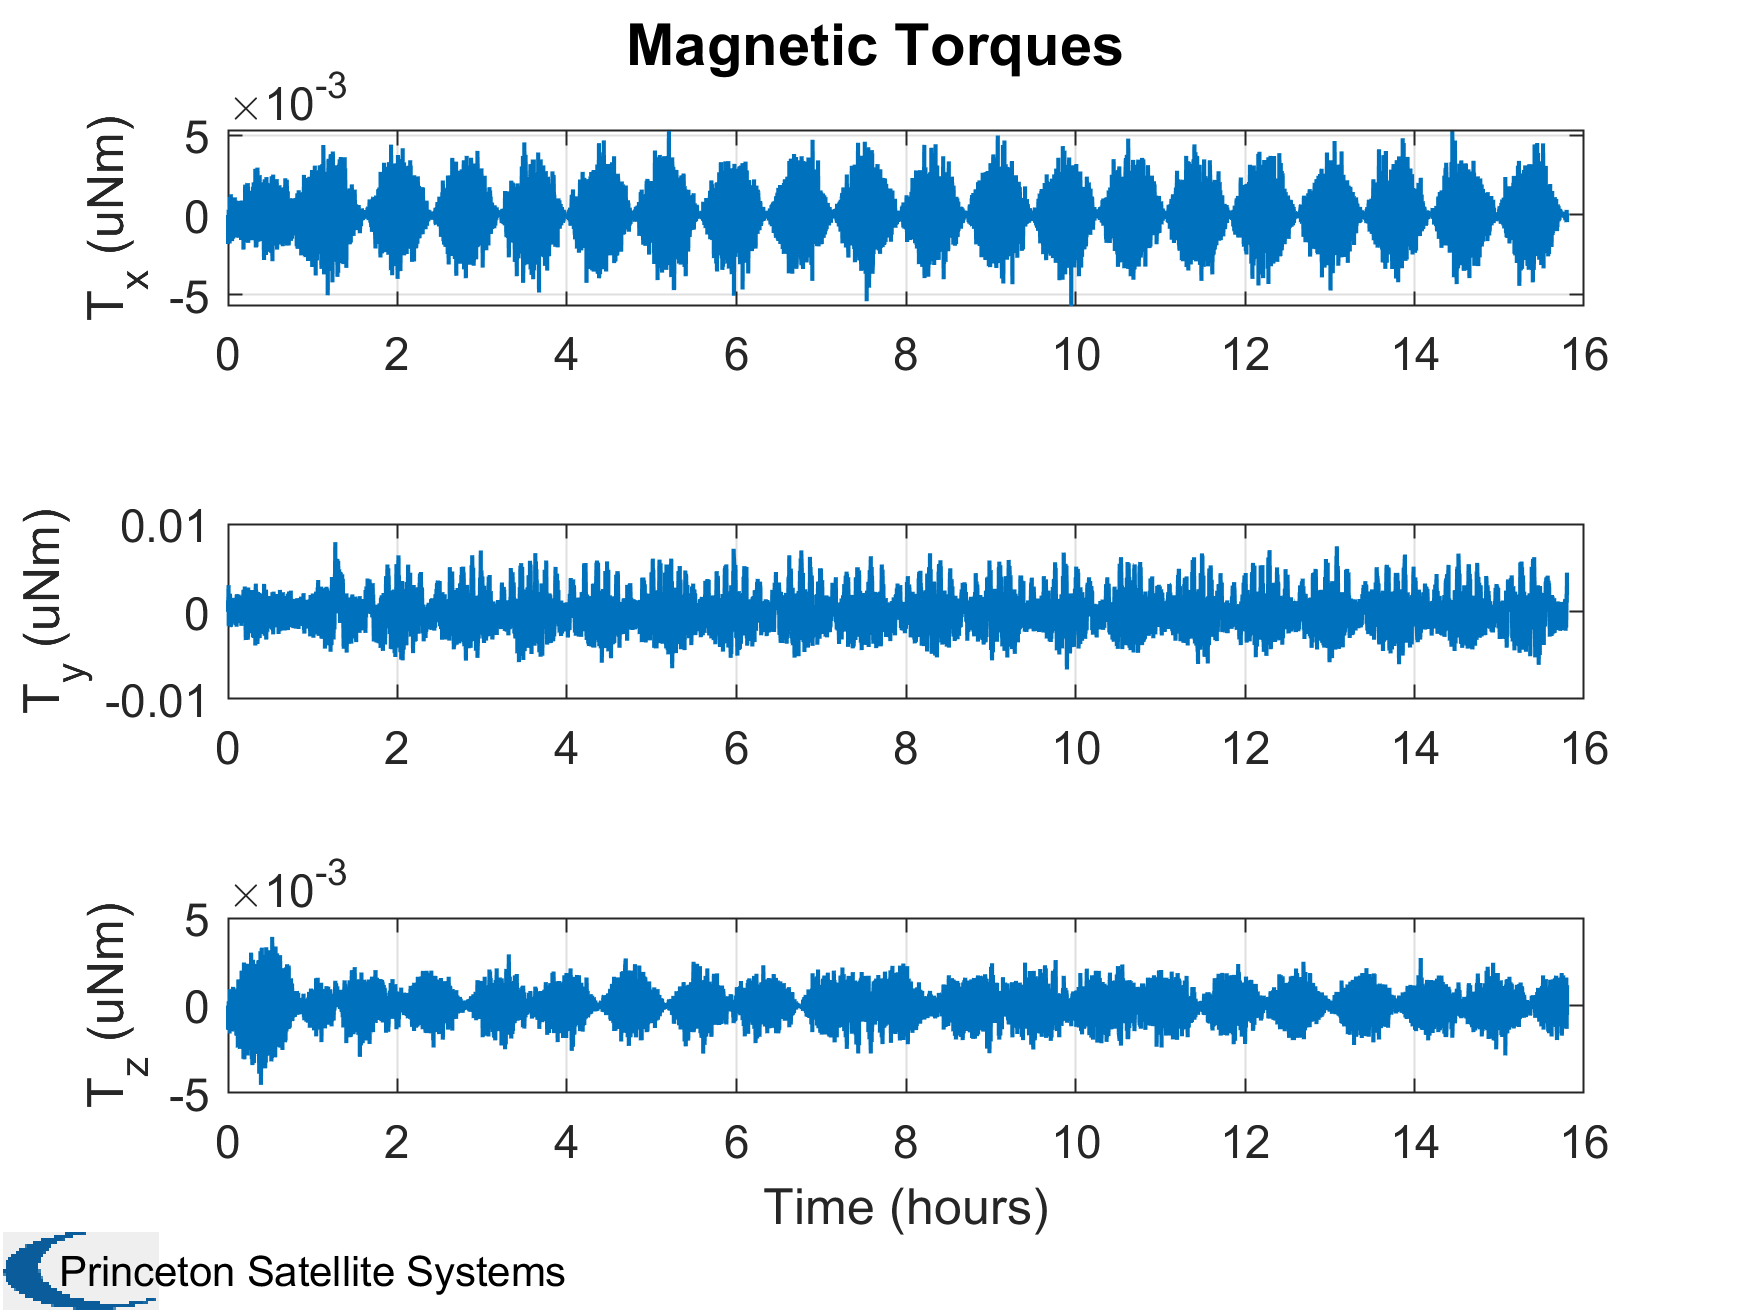
\includegraphics[width=0.48\linewidth]{res/img/Nadir_EKF/Simulations/Magnetic Torques.png}
        \caption{Magnetic Torques}
    \end{figure}

    \item \textbf{Injected Intensity}\\
    This section illusttrates the requrired intensity to be injected in the magnetorquers in order to generate the necessary
    magnetic moment to conduct the Nadir Pointing mode. 
    \begin{figure}[H]
        \centering
        \begin{minipage}{0.32\linewidth}
            \centering
            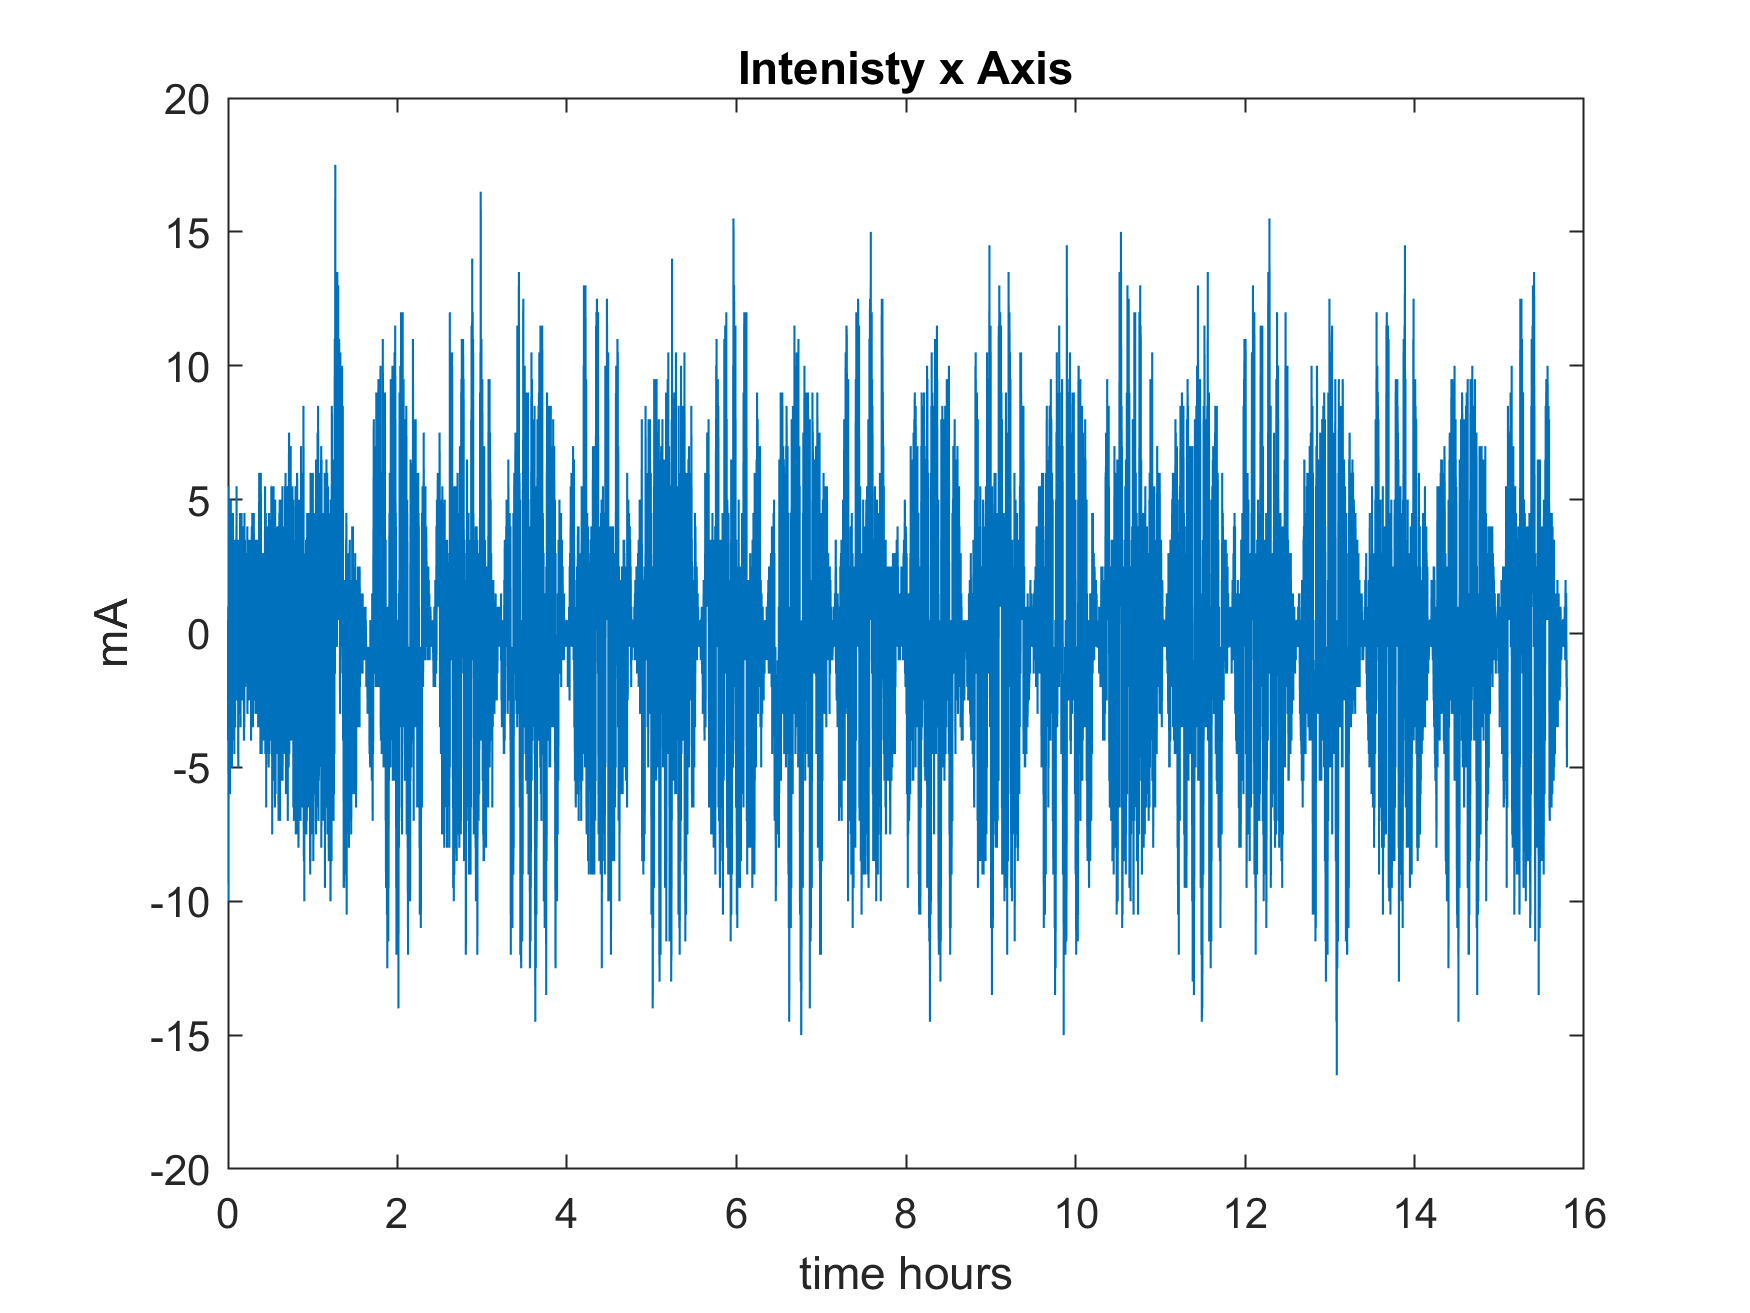
\includegraphics[width=0.95\linewidth]{res/img/Nadir_EKF/Simulations/Intenisty x Axis.png}
            \caption{Intensity x Axis}
            \label{fig:IntensityX}
        \end{minipage}\hfill
        \begin{minipage}{0.32\linewidth}
            \centering
            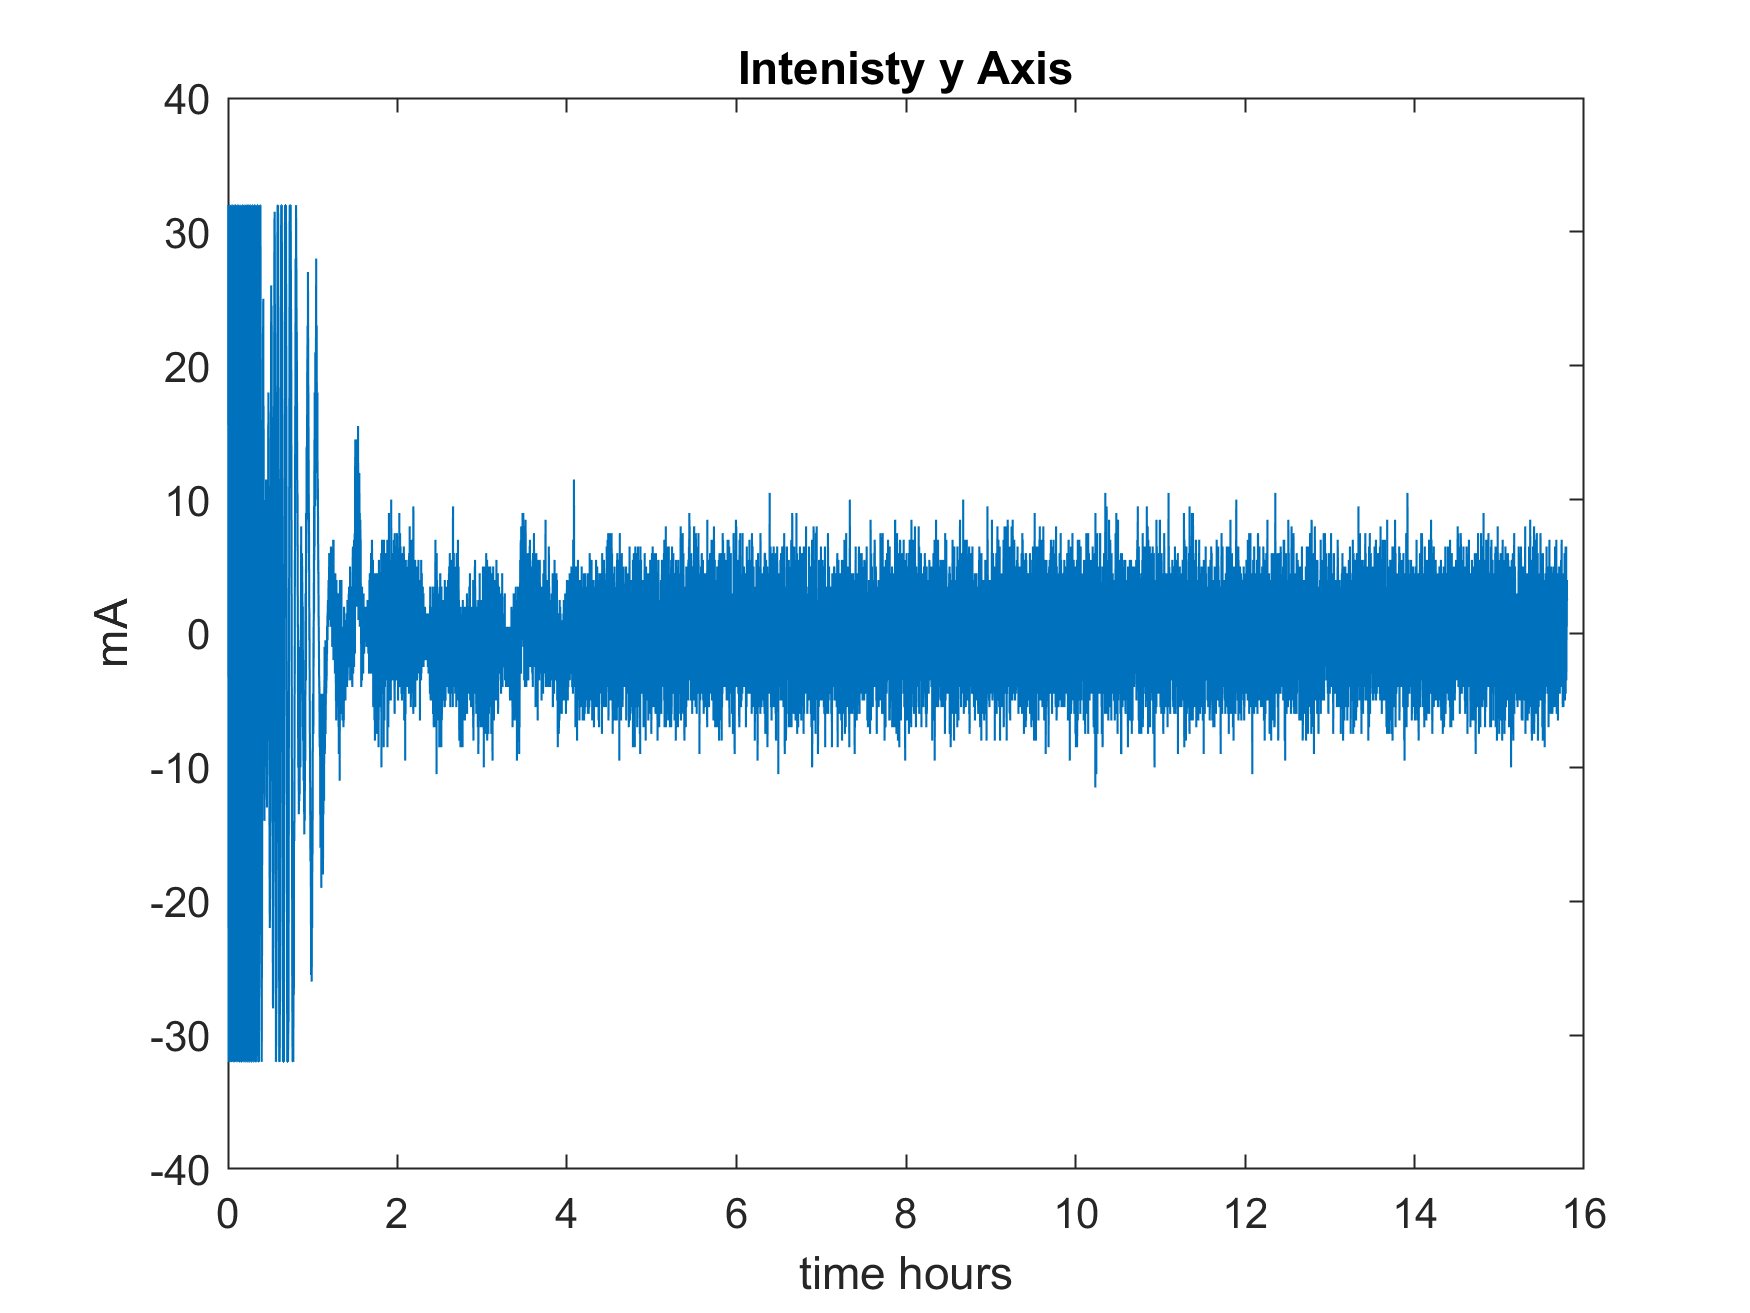
\includegraphics[width=0.95\linewidth]{res/img/Nadir_EKF/Simulations/Intenisty y Axis.png}
            \caption{Intensity y Axis}
            \label{fig:IntensityY}
        \end{minipage}\hfill
        \begin{minipage}{0.32\linewidth}
            \centering
            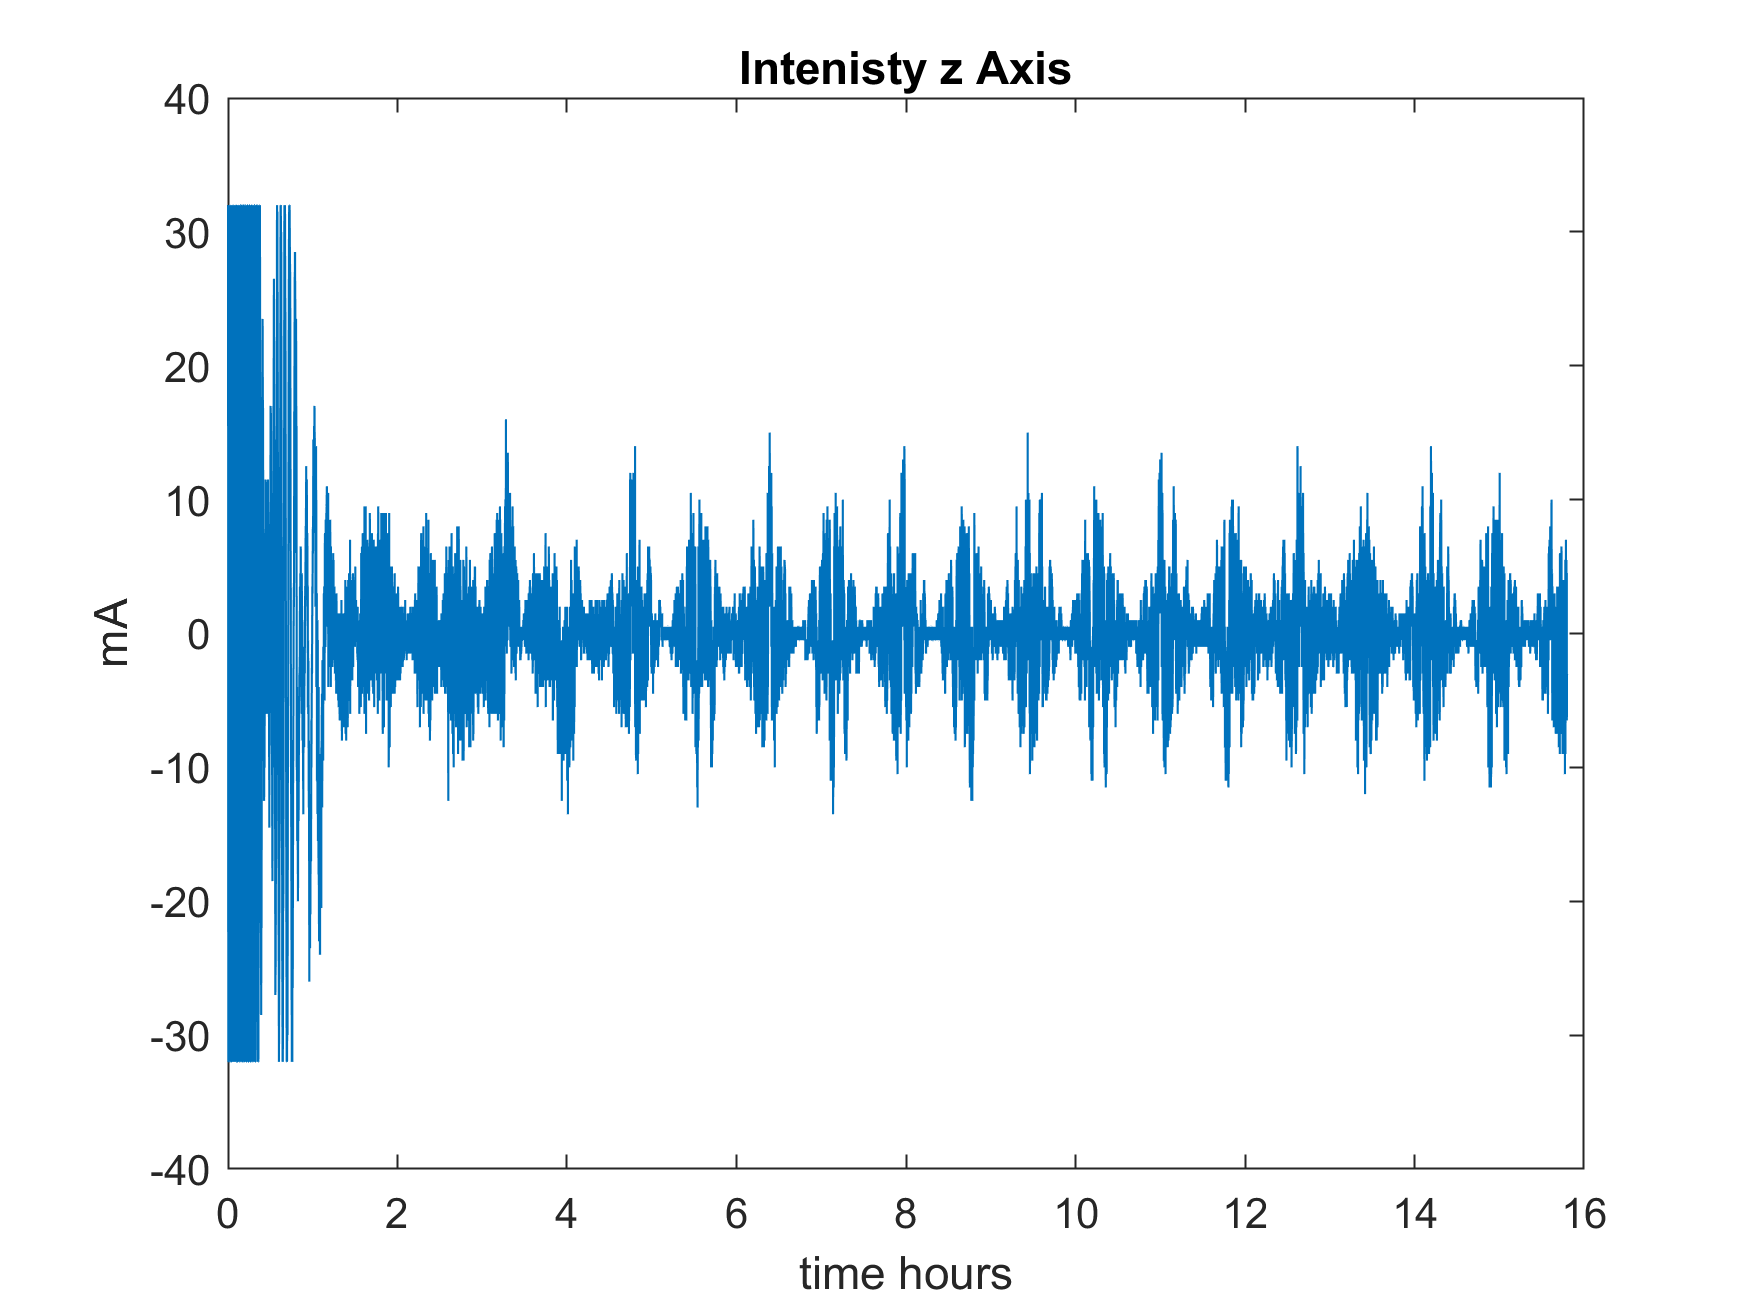
\includegraphics[width=0.95\linewidth]{res/img/Nadir_EKF/Simulations/Intenisty z Axis.png}
            \caption{Intensity z Axis}
            \label{fig:IntensityZ}
        \end{minipage}
    \end{figure}

    \item \textbf{Attitude quaternion}\\
    In this section the attitude quaternion of the PQ estimated by the EKF is presented. A comparative between the 
    quaternion estimated by the EKF and the quaternion estimated by the simulation without the EKF will be presented in later sections.
    \begin{figure}[H]
        \centering
        \includegraphics[width=0.7\linewidth]{res/img/Nadir_EKF/Simulations/LVLH To Body Quaternion.png}
        \caption{LVLH To Body Quaternion}
    \end{figure}

    \item \textbf{EKF Performance}\\
    To assess the performance of the EKF, a performance campaign has been conducted. The campaign consists of 20 simulations using the same
    initial state and orientation of the PQ. After each simulation the orientation of the PQ is extracted by means of the quaternion
    describing the rotation from the LVLH frame to the body frame. Finally that quaternion is used to calculate
    the mean square error (MSE) of each quaternion component, so that the performance of the EKF can be evaluated. In order to compute the MSE, the ideal
    quaternion used is the quaternion [1, 0, 0, 0], which represents the ideal attitude of the PQ in the Nadir Pointing mode.\\
    
    The first plot shows the quaternion evolution for the 20 simulations, where it can be observed that in overall, all the quaternion components
    manage to converge aproximately to the ideal quaternion.

    \begin{figure}[H]
        \centering
        \includegraphics[width=1\linewidth]{res/img/Nadir_EKF/EKF_performance/20_SIM_quat.png}
        \caption{Quaternion evolution for 20 simulations}
        \label{fig:EKF_20_SIM_quat}
    \end{figure}

    The following plots show the MSE of each quaternion component. Additionally, the bias$^2$, the variance and the first component
    of the covariance matrix are also presented.

    In the first plot, the component $q_1$ of the quaternion is presented, which is the scalar component of the quaternion. In this case,
    it can be observed that the variance is in most of the plot with a very aproximated value to the MSE. That means that the EKF in that
    component is working extremely close the optimal estimator. It is good to take into account that as an EKF is being used, the fact of 
    having to linearize the system makes complex to obtain an ideal optimal estimator (variance = MSE).  
    \begin{figure}[H]
        \centering
        \includegraphics[width=\linewidth]{res/img/Nadir_EKF/EKF_performance/performance q1.png}
        \caption{Performance $q_1$}
        \label{fig:EKF_PerformanceQ1}
    \end{figure}

    In the following three plots, the components $q_2$, $q_3$ and $q_4$ of the quaternion are presented. In this case these components
    are more valuable for obtaining a better nadir pointing performance. Firstly, in all plots can be observed two different phases, 
    on the one hand, the first phase in which the EKF tries to reduce the angular velocity to 0 and tries to point as close as possible to 
    the nadir vector. In this phase the EKF as can be seen works as the optimal estimator, as the variance is very close to the MSE. This happens
    because the EKF detects that the covariance matrix variates in time, thus the EKF tries to reduce the MSE and as a 
    consequence the variance to achieve a more constant covaraince matrix. In order to do that, the EKF assigns more confidence in the measurements 
    than in the predictions.

    In the second phase, once the angular velocity has been significantly reduced and the attitude has converged near the nadir direction, 
    the EKF enters a tracking or steady-state phase. At this point, the estimation no longer requires aggressive corrections. This is reflected in 
    the covariance matrix, which becomes more stable and varies less over time.
    Since the EKF assumes the system is already well-aligned with the nadir direction, it relies more heavily on its predictions rather than the incoming measurements. 


    \begin{figure}[H]
        \centering
        \includegraphics[width=\linewidth]{res/img/Nadir_EKF/EKF_performance/performance q2.png}
        \caption{Performance $q_2$}
        \label{fig:EKF_PerformanceQ2}
    \end{figure}

    \begin{figure}[H]
        \centering
        \includegraphics[width=\linewidth]{res/img/Nadir_EKF/EKF_performance/performance q3.png}
        \caption{Performance $q_3$}
        \label{fig:EKF_PerformanceQ3}
    \end{figure}

    \begin{figure}[H]
        \centering
        \includegraphics[width=\linewidth]{res/img/Nadir_EKF/EKF_performance/performance q4.png}
        \caption{Performance $q_4$}
        \label{fig:EKF_PerformanceQ4}
    \end{figure}
    

\end{itemize}

\subsection{Detumbling mode}